The medical community, typically, has been established to take care of human health with knowledgeable and expert clinicians, like radiologists, hematologists, or health science specialists. Nowadays, technology provides an opportunity for having faster and more accurate tools, e.g., X-ray machines, CBC machines, and MRI. These automated medical tools are essential for diagnosing patients' health conditions. In this context, CAD systems have recently gained attention because they could offer a valid help to clinicians. They have to deal with different medical fields and with issues related to images and data to manage. In particular, CAD systems dealing with images acquired with a digital microscope have to face additional issues like the variations of illumination and acquisition conditions or the different types of smear staining. Despite the previously listed issues, CAD systems for digital microscope based on image processing techniques generally consist of the following phases:
\begin{itemize}
	\item Image pre-processing: noise suppression added to the image during the phase of acquisition and improvement of the luminance and contrast of the images.
	\item Segmentation: partitioning the image to isolate the objects of interest in the image. This phase is the most important in the automatic analysis of images, as from the result of the segmentation depends on the result of the entire analysis.
	\item Feature extraction: feature extraction of previously segmented objects, necessary for subsequent classification.
	\item Classification: assignment of segmented objects to a specific class. If present, any disease is determined through this phase.
\end{itemize}

In general, it is possible that some CAD systems do not need to use all the mentioned phases. As an example, pre-processing could be avoided if images have been captured with the most recent microscopes which produce high-quality images with a low percentage of imperfections or artifacts. Conversely, some phases can be repeated multiple times in order to deal with different issues. For instance, performing numerous stages of segmentation is very frequent in peripheral blood smear images analysis, for example using the first segmentation to firstly identify the cells and then to separate the components of the cells themselves. 
The following chapters give an overview of the most used techniques in the different phases of a typical CAD system and the basic concepts applied to the proposed methods for peripheral blood image analysis, described in part \ref{due} will be depicted.

\chapter{Image Pre-processing}
\label{preproc}
Pre-processing is a common name for operations with images at the lowest level of abstraction.
The primary purpose is an improvement of the image condition by means of some operations in order to suppress unwanted distortions, such as noise or artifacts, or enhance some image features for further processing like, for example, enhancing or stretching the contrast, separating, in a better way, the objects of interest from the background.
It is worth to indicate that pre-processing methods may be unnecessary on CAD systems for several reasons: first of all, image acquisition tools, like modern microscopes, are equipped with high-level cameras, and they can produce excellent quality images. Secondarily, this kind of operations could alter a lot, or even suppress, the structures of the cells which are essential for further analysis phases. Typically, images structures are represented with an appropriate definition with only a small quantization noise, or they can directly be acquired in a low contrast environment. For these reasons the most used pre-processing operations are:
\begin{itemize}
	\item Histogram operations
	\item Local pre-processing operations:
	\begin{itemize}
		\item Smoothing operators
		\item Sharpening operators
	\end{itemize}
\end{itemize}

\section{Operations on the histogram}\label{histop} % DONE
An image histogram is a representation of the tonal distribution in a digital image. A good example is the grey level histogram. It provides the frequency of pixels' intensity values inside the image and indicates the number of pixels having each grey level. 
It also gives useful information about the image, such as the number of modes, the presence of a dominant peak or the grey levels distribution along the histogram. If the image has a low contrast, it means that all the pixels values are condensed towards a side of the histogram. On the other hand, a bimodal histogram often denotes the presence of a fairly homogeneous brightness object on a nearly constant background. Operating on the histogram means defining a mapping $h$ from the initial space of grey levels in a new grey levels space $h: [0..255] \rightarrow [0..255]$, whose application to the image $I$, is the replacement of grey level $I[i, j]$ with $h(I[i, j])$. Therefore, it is possible to increase the contrast within the image, equalize the histogram and highlight or hide some image details, by defining the appropriate mapping.
The \textit{contrast stretching} operation is necessary when the histogram values are not distributed over the entire frequency range. Stretching the histogram is a solution to correct this situation, by mapping the minimum and the maximum value of the original image with the value $0$ and $255$, respectively. This operation is common for cytometric image analysis, as it allows good separation of foreground objects from the background. Figure \ref{fig:contrastStretching} shows an example of contrast stretching.
The \textit{histogram equalization} operation is essential because it is often used to make images captured in different lighting conditions comparable. The equalization is achieved by defining a mapping that equally distributes the pixels values. This operation produces a histogram (theoretically) flat, considering $h(x)$ as the histogram of the original image, it can be changed through the use of the function $y = y(x)$, so that the histogram $g(y)$ of the resulting image becomes constant for each intensity value $g(y) = c$.

\begin{figure}[!h]
	\centering
	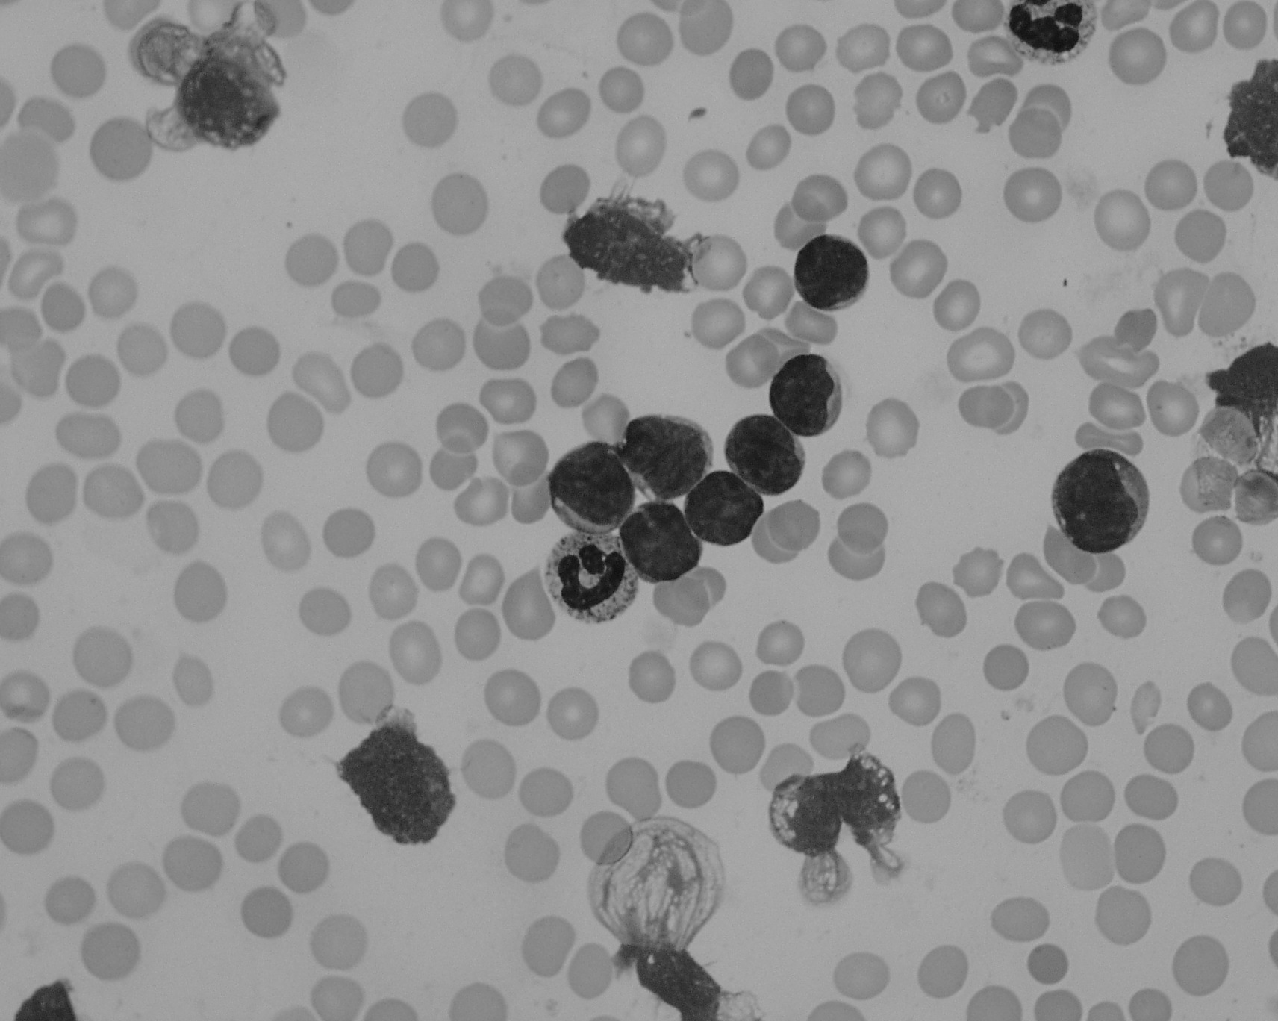
\includegraphics[width=0.3\textwidth]{images/figContrastStretching1}
	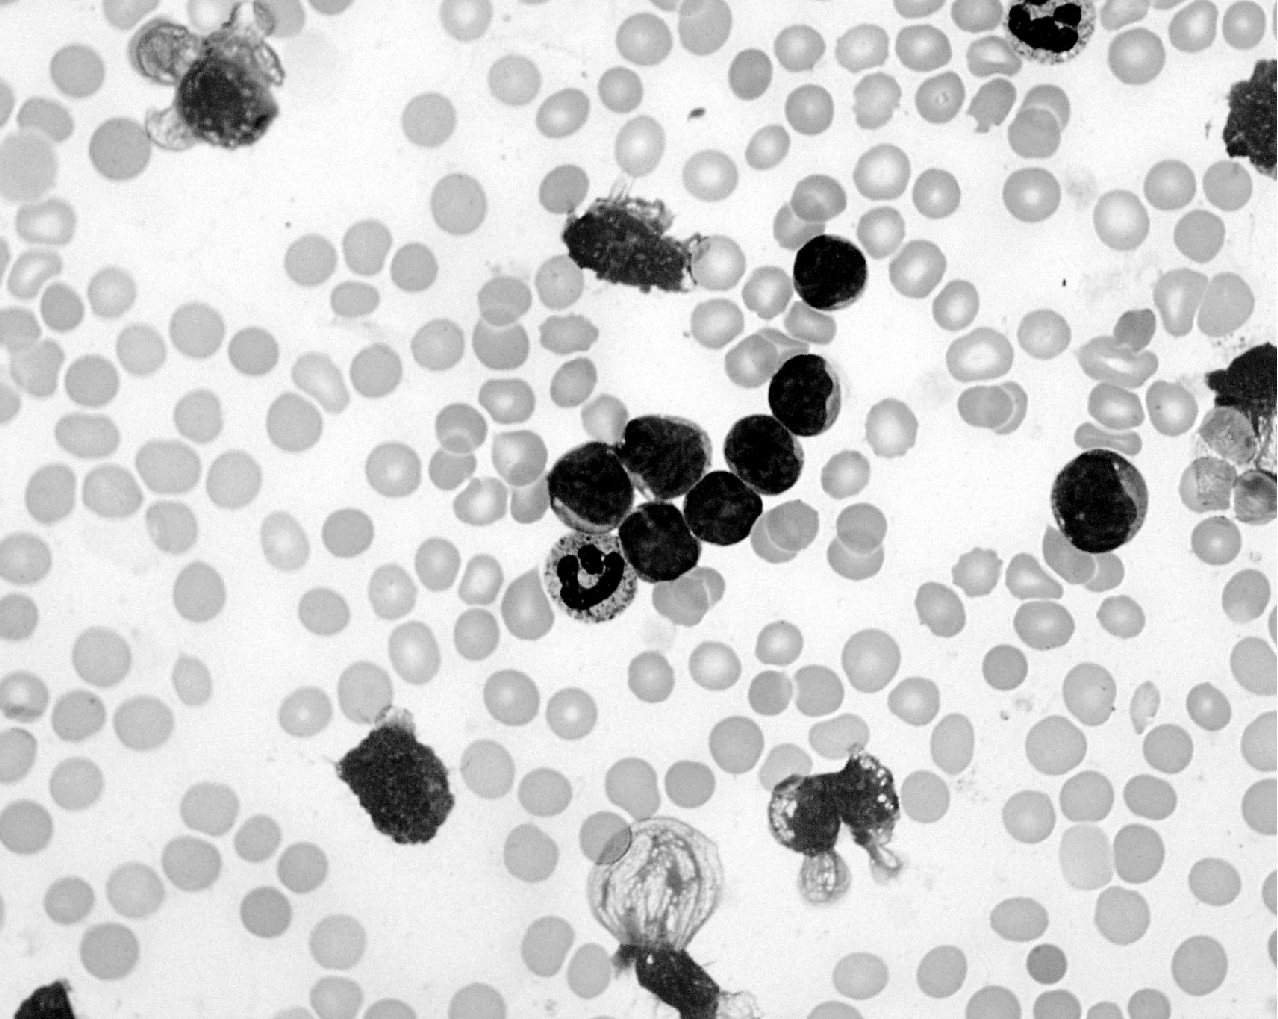
\includegraphics[width=0.3\textwidth]{images/figContrastStretching2}
	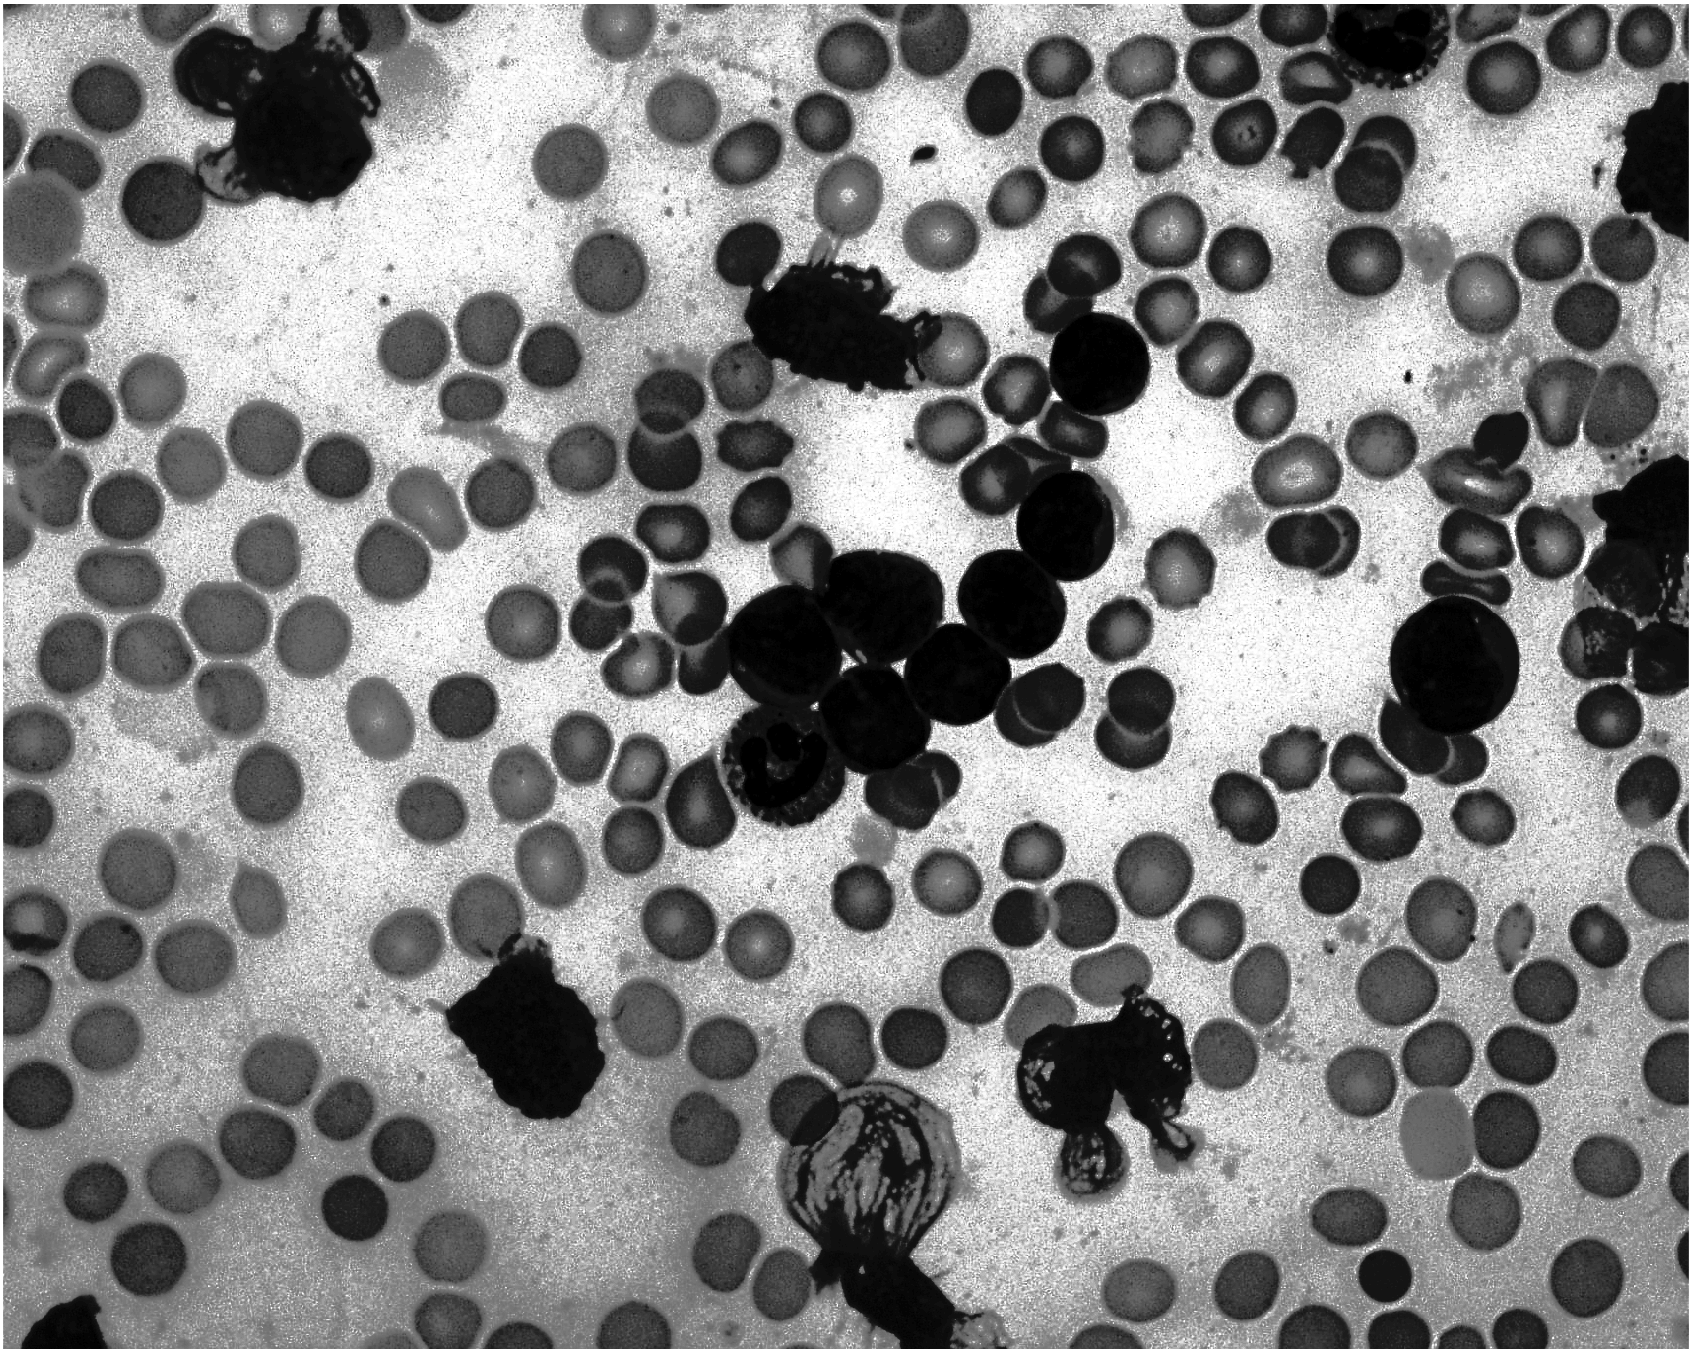
\includegraphics[width=0.3\textwidth]{images/figHistogramEqualization}
	\caption[Example of operations on the histogram.]{\label{fig:contrastStretching} Example of operations on the histogram. Left: original greyscale image. Center: contrast stretched image. Right: result of histogram equalization with 64 bins.}
\end{figure}

\section{Operations of local pre-processing} % DONE
Local pre-processing ones operate on a small neighborhood of the original image pixels to calculate new pixel values of the resulting image rather than on the entire image. They are also called filtering operations since they make use of digital filters. The pixels neighborhood, used to calculate new intensity value, always needs to have odd cardinality, in such a way that the considered pixel lies in the middle of the neighborhood. Typically, the sizes are $3\times3$, $5\times5$ or $7\times7$. The filter used for the filtering operation has the same size as the considered pixel's neighborhood. The values of the filter are used as a weight that is multiplied by the corresponding pixel values of the neighborhood and then added together to give rise to the new value of the pixel in the resulting image. We can distinguish between two groups of local pre-processing methods, in accordance with their ultimate goal. They are the smoothing and the sharpening operators.

\subsection{Smoothing operators} % DONE
The smoothing operators have the purpose of suppressing noise or other small unwanted details in images, using their redundancy. Unfortunately, as previously said, these operators tend to flatten also useful details such as objects' edges and the cell structures, even though they generally produce good results in the removal of impulsive noise. The most used smoothing operator is the \textit{averaging filter}. It stores the average value of its neighborhood in the considered pixel. In this case, the results are acceptable if the noise has a smaller size than the objects of interest; in any case, the objects' contours are heavily altered. Average filters can also have different weight values, to properly reflect the characteristics of the Gaussian noise. They are also called Gaussian filters since they simulate the trend of a Gaussian curve. Fig. \ref{fig:smoothing} represents an example. Another common smoothing operator is the \textit{median filter}, which behaves similarly to the average filter. The only difference is that it stores the median value of its neighborhood in the considered pixel.

\begin{figure}[!h]
	\centering
	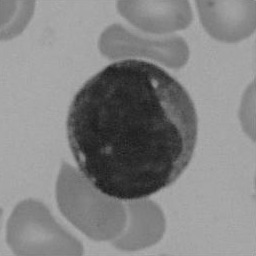
\includegraphics[width=0.24\textwidth]{images/smooth0}
	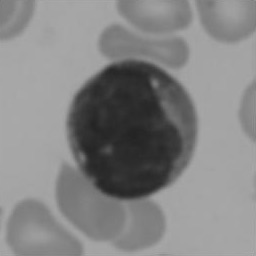
\includegraphics[width=0.24\textwidth]{images/smooth1}
	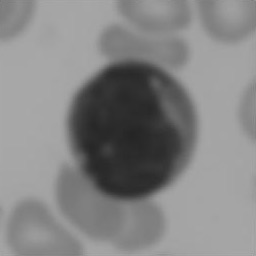
\includegraphics[width=0.24\textwidth]{images/smooth2}
	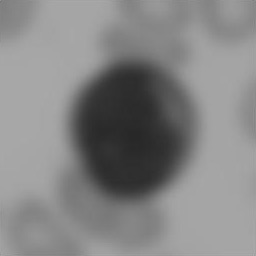
\includegraphics[width=0.24\textwidth]{images/smooth3}
	\caption[Example of Gaussian smoothing filter.]{\label{fig:smoothing}Example of Gaussian smoothing filter application on a grey level image. From left to right: original greyscale image, filtered images with $\sigma$ = 2, 4 and 8.}
\end{figure}

\subsection{Sharpening operators} % DONE
The sharpening operators have the purpose of highlighting the interesting details of the image, such as the edges of objects. Unfortunately, these operators tend to highlight also the noise present in the image, however they improve the perceived picture detail. These operators depend on the use of local derivatives of the image. Since the image is a discrete function, the traditional definition of derivative cannot be applied.
In digital images, the operator used for the first derivative is the intensity difference between adjacent pixels. In most cases, the sharpening operators use the second derivatives, since they are more sensitive to intensity variations. The most used sharpening operator is the \textit{Laplacian filter} that brings the desired sharpening effect by subtracting the Laplacian filtered image from the original one. Another useful sharpening operator is the \textit{gradient operator} that makes use of the image gradient to detect and improve the edges. An edge is a set of connected pixels (4 or 8 connected) with sharp changes in brightness, so it can be detected as any transition of grey levels, where the slope of this transition is proportional to how the edge is sharp. Such image function change can be described by the gradient pointing in the direction in which the function has its most significant growth. Prewitt, Sobel, Kirsch, and Robinson are examples of operators that can correctly determine the gradient direction by using the first derivative. Another common sharpening operator used in most of the commercial products to make the image noticeably sharper is the \textit{Unsharp} filter. It is a simple sharpening operator which takes its name from the fact that it enhances edges and other high-frequency components in an image via a procedure that subtracts a smoothed (or unsharp) version of the image from the original one. Fig. \ref{fig:sharpening} shows some examples of the described sharpening operators.

\begin{figure}[!h]
	\centering
	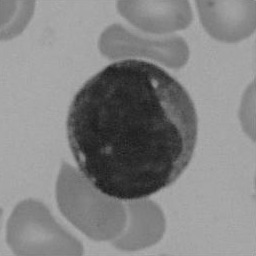
\includegraphics[width=0.24\textwidth]{images/smooth0}
	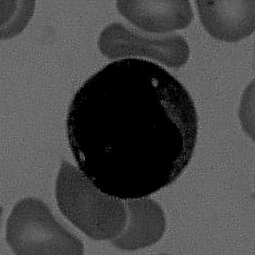
\includegraphics[width=0.24\textwidth]{images/sharpen1}
	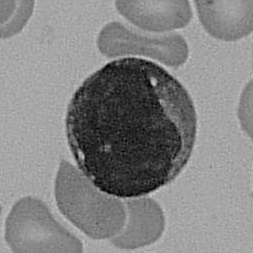
\includegraphics[width=0.24\textwidth]{images/sharpen2}
	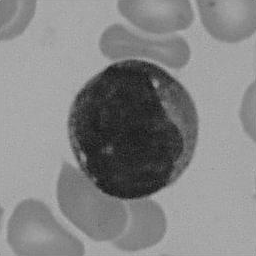
\includegraphics[width=0.24\textwidth]{images/sharpen3}
	\caption[Example of sharpening operators.]{\label{fig:sharpening}Example of sharpening operators. From left to right: original greyscale image, application of Laplacian filter, gradient operator and unsharp filter.}
\end{figure}

\section{Color and Color Spaces} 
Color is very important in CAD systems since the hematologists stain blood to highlight spatial structures. The color is the brain's reaction to a specific visual stimulus. It is incredibly subjective and personal, thus trying to attribute numbers to the brains reaction to visual stimuli is very difficult. Color spaces aim to aid the process of describing the colors, either between people or between machines or programs. The presence of more than one color space is since different color spaces can work better in specific applications, for example, some devices have limiting factors that dictate the size and type of color space used. Thus, some color spaces are tied to a specific piece device (device dependent) while others are equally valid on whatever device they are used (device independent). The standard families are primary, luminance-chrominance, and perceptual spaces  \cite{Vandenbroucke, Busin} and they classify color spaces into a few categories, concerning their definitions and their properties.

\subsection{Primary Spaces}  
The primary spaces are based on the trichromatic theory of color vision, also known as the Young-Helmholtz theory of color vision. It states that there are three receptors in the retina that are responsible for the perception of color. One receptor is sensitive to the color green, another to the color blue and a third to the color red. These three colors can then be combined to form any visible color in the spectrum.
The primary spaces assume that it is possible to match any color by mixing appropriate amounts of the three primary colors. Examples of primary spaces are the real RGB, the subtractive CMY(K), and the imaginary XYZ. The most widely used color space indeed is the RGB color space, in which a color point in the space is characterized by three color components of the corresponding pixel which are red (R), green (G), and blue (B). In general, color images are acquired through the RGB color space, called the image acquisition color space. Therefore, all the color spaces are expressed thanks to transformations performed on the R, G and B channels.
As previously said, CMY(K) is the subtractive color space and can be obtained easily from a set of RGB values by subtracting the individual RGB values from 1, since a pure cyan (C) surface does not contain R, a pure magenta (M) surface does not contain G and a pure yellow (Y) surface does not contain B. So, the equation is:

\begin{equation}
\left [ { \begin{array}{c} C  \\ M   \\ Y \end{array} } \right ] = 
\left [ { \begin{array}{c} 1   \\ 1   \\ 1 \end{array} } \right ]  - \left [ { \begin{array}{c} R  \\ G  \\ B     \end{array} } \right ] 
\end{equation}
\\
with the assumption that, in general, all color values have been normalized to the range $[0,1]$. In general, this color space is used in color printers and copiers that internally perform this conversion. According to the equation, equal amounts of the color channels should produce black. In practice, however, their combination for printing produces only a dark color far from the real black. Thus, to produce a pure black a fourth color has been added, giving rise to the CMYK color space. In this case, the conversions start from the just computed CMY, by finding the black (K) channel and then correcting the complementary colors based on the value of K.

\begin{equation}\label{cmyk}
\begin{split}
&K = minimum (c, m, y)\\
&C = c - K\\
&M = m - K\\
&Y = y - K\\
\end{split}
\end{equation}

The XYZ colour space is obtained from the RGB colour space using the following equation:

\begin{equation}
\left [ { \begin{array}{c} X  \\ Y   \\ Z \end{array} } \right ] = 
\left [ { \begin{array}{c c c} \mbox{ 0.412}  & \mbox{ 0.357} &  \mbox{ 0.180 } \\ \mbox{ 0.212} & \mbox{ 0.715} & \mbox{ 0.072 } \\ \mbox{ 0.019} & \mbox{ 0.119} & \mbox{ 0.950 }  \end{array} } \right ] \cdot \left [ { \begin{array}{c} R  \\ G  \\ B     \end{array} } \right ] 
\end{equation}

\begin{figure}[!h]
	\centering
%	\hspace{-2.6mm}
	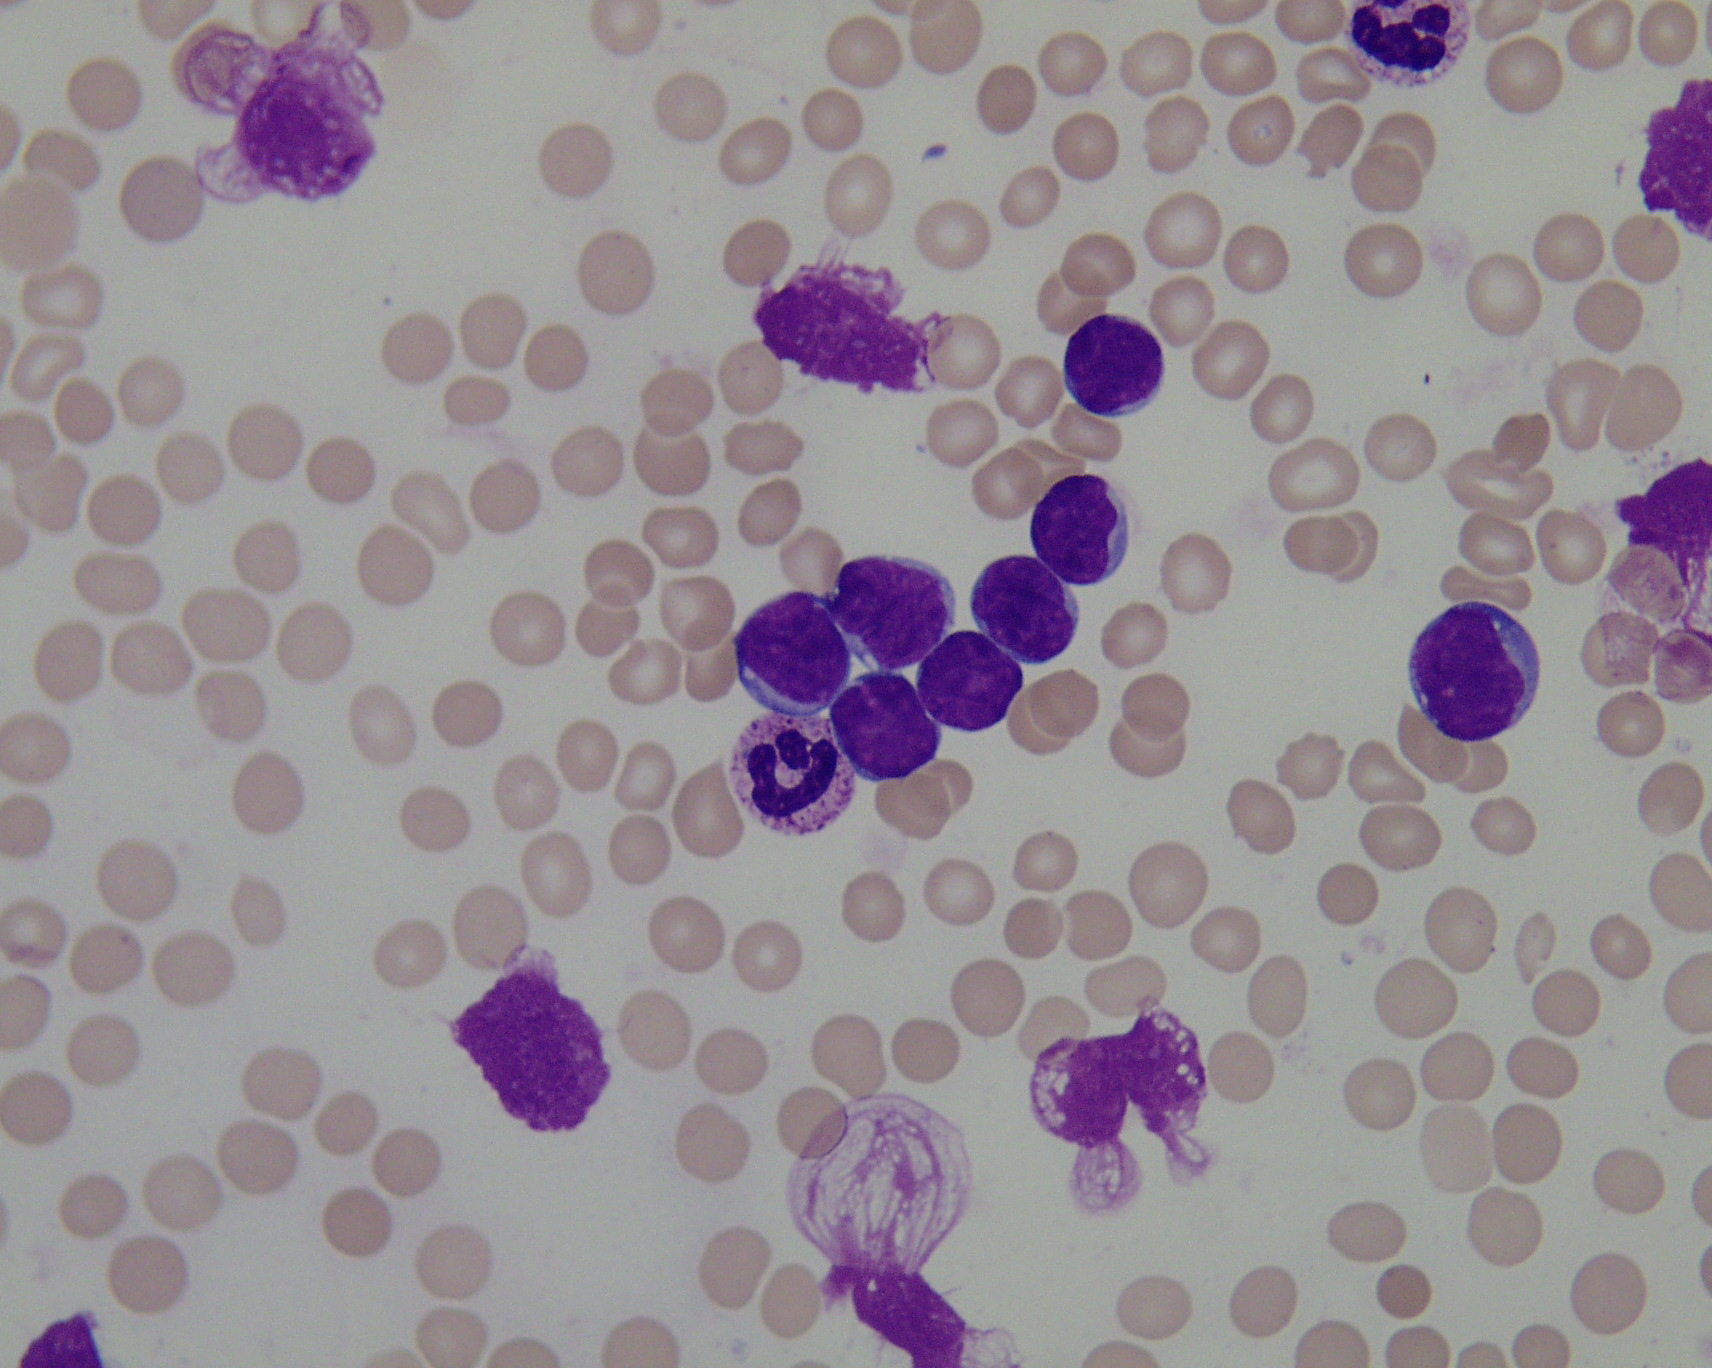
\includegraphics[width=0.3\textwidth]{images/figcs_rgb}
	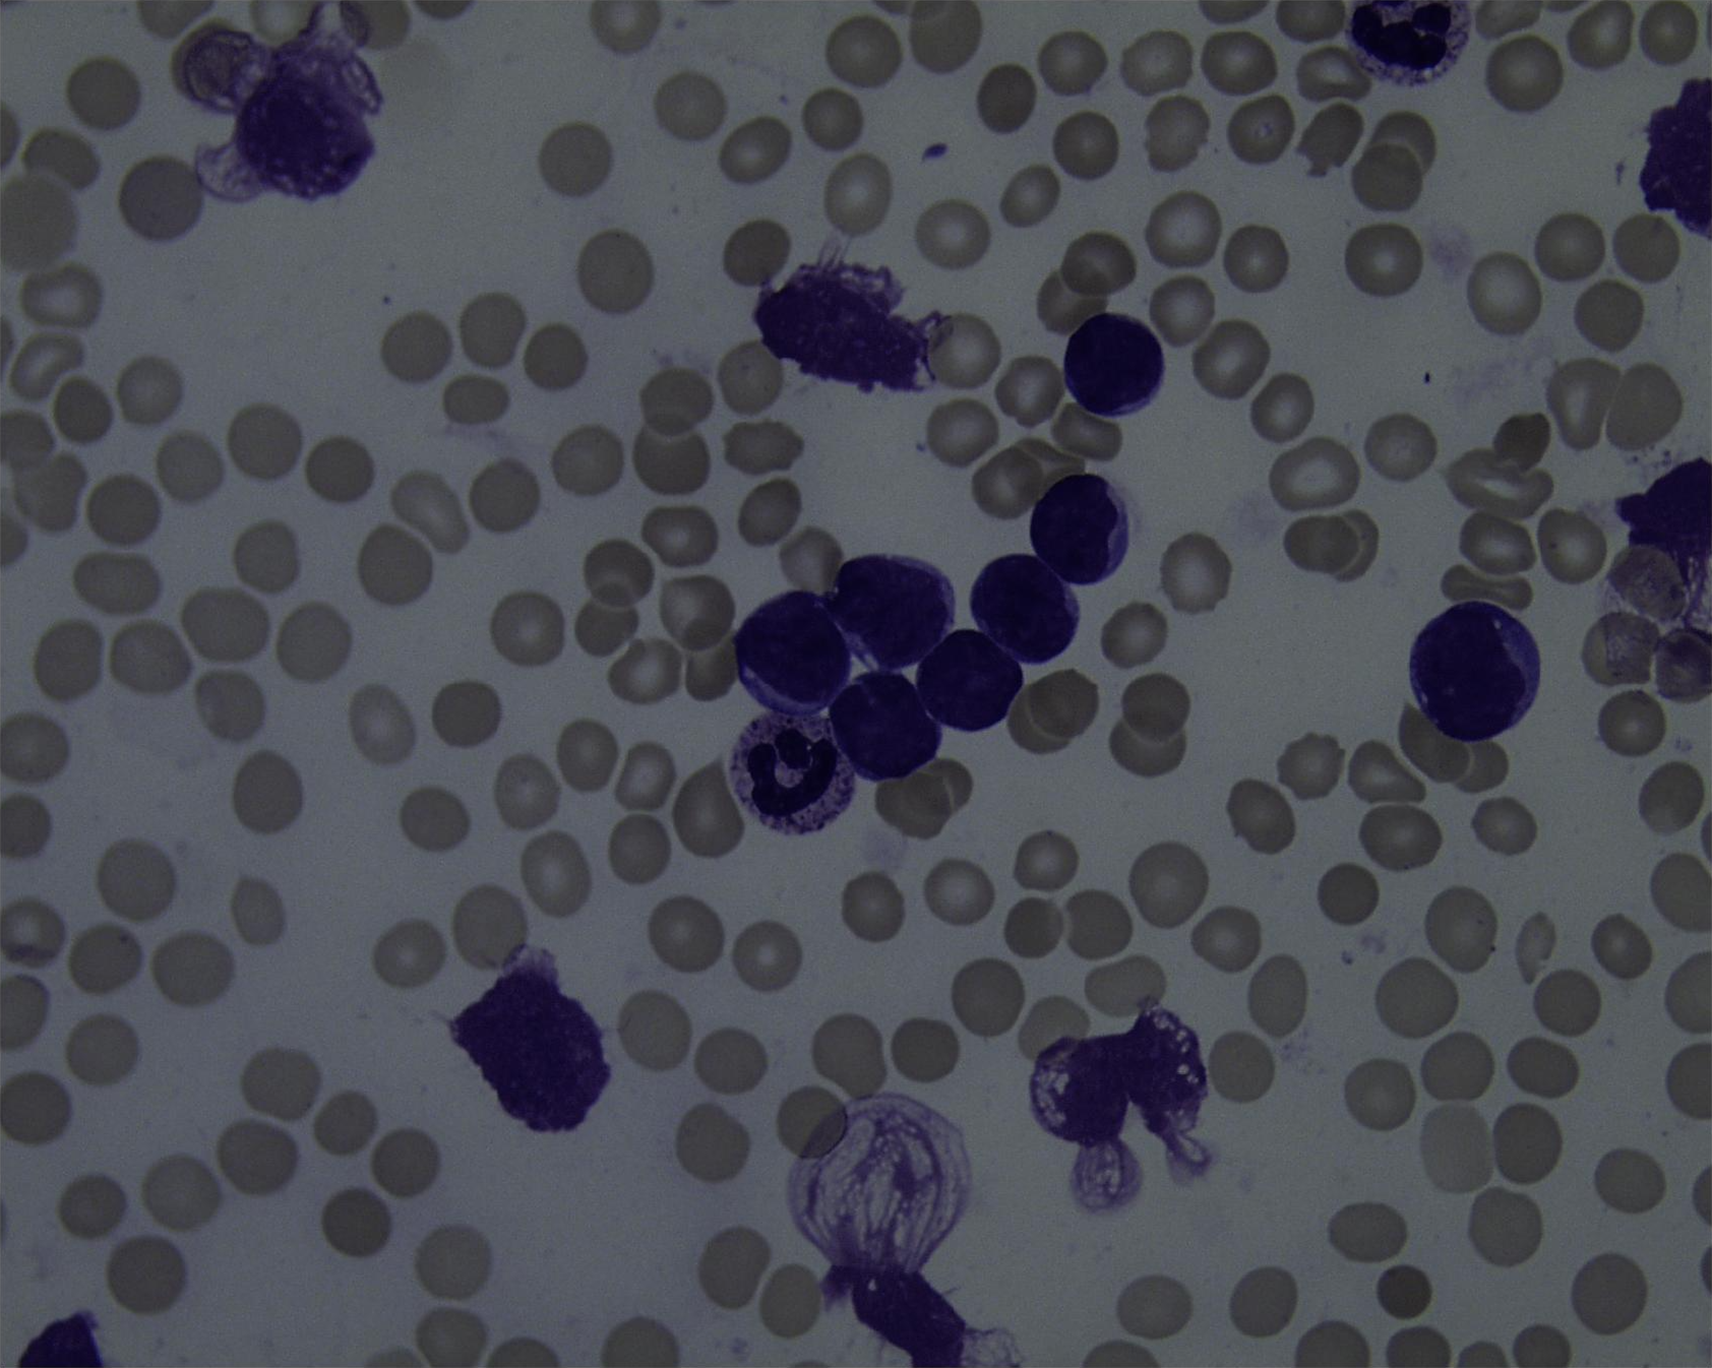
\includegraphics[width=0.3\textwidth]{images/figcs_xyz}
	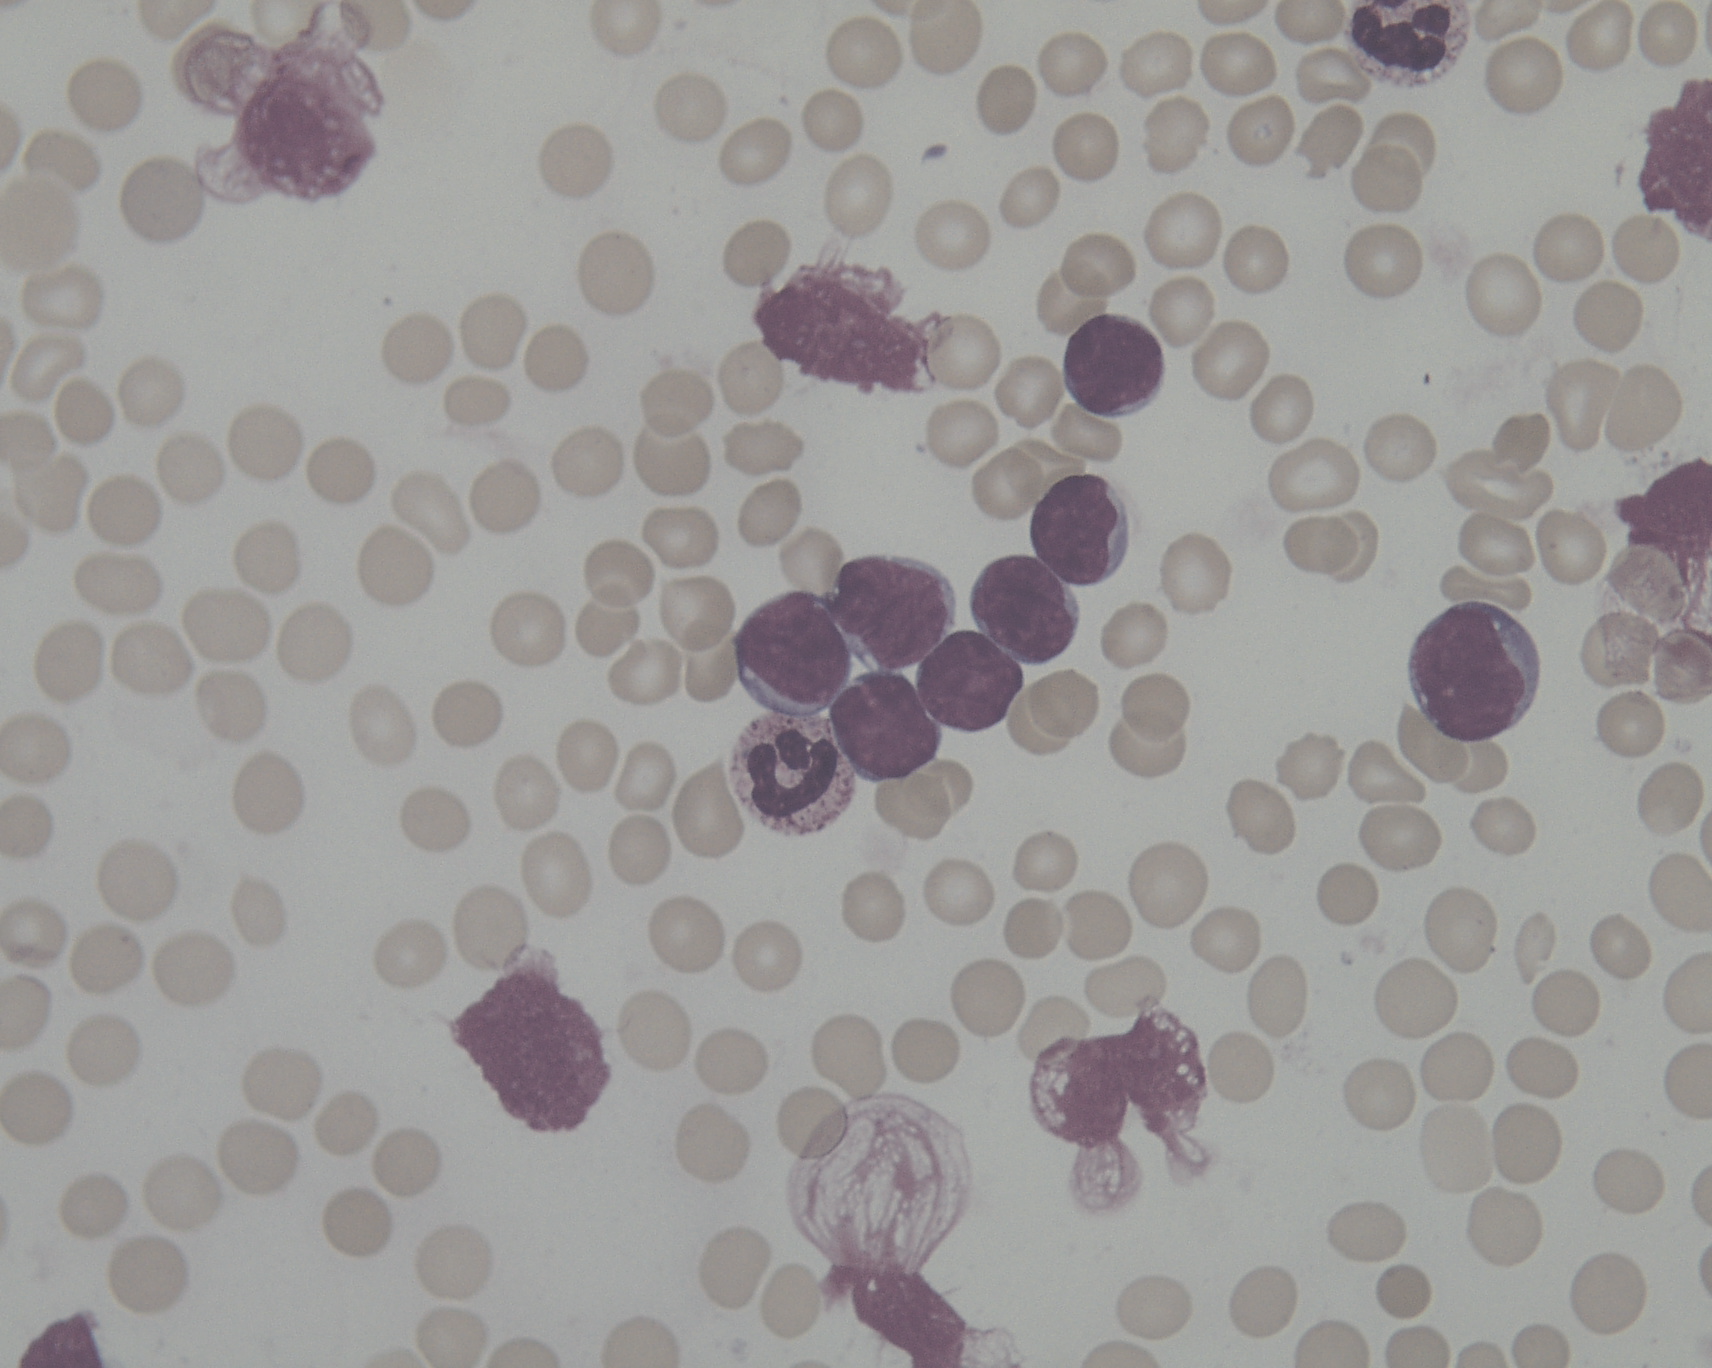
\includegraphics[width=0.3\textwidth]{images/figcs_cmyk_all}
	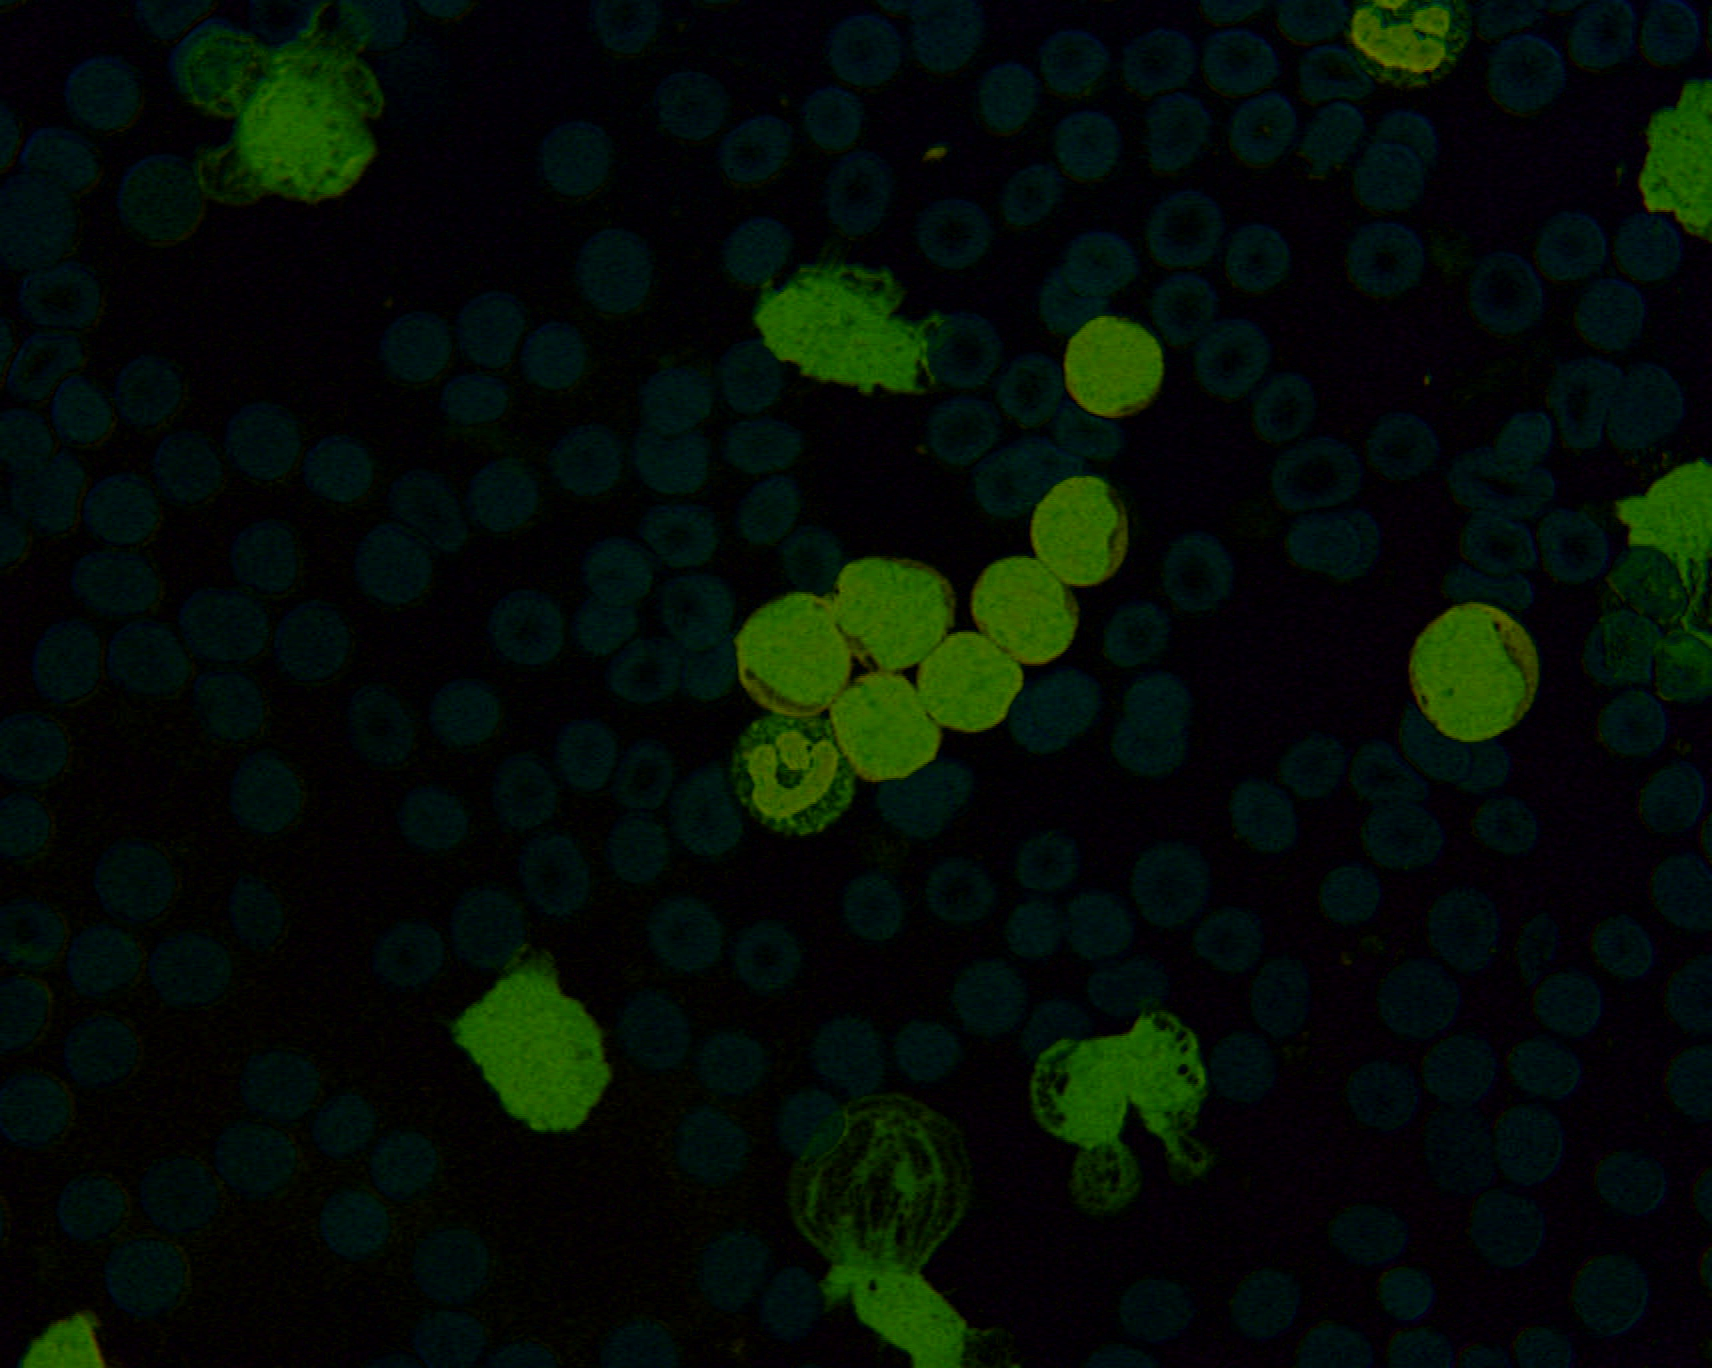
\includegraphics[width=0.3\textwidth]{images/figcs_cmyk123}
	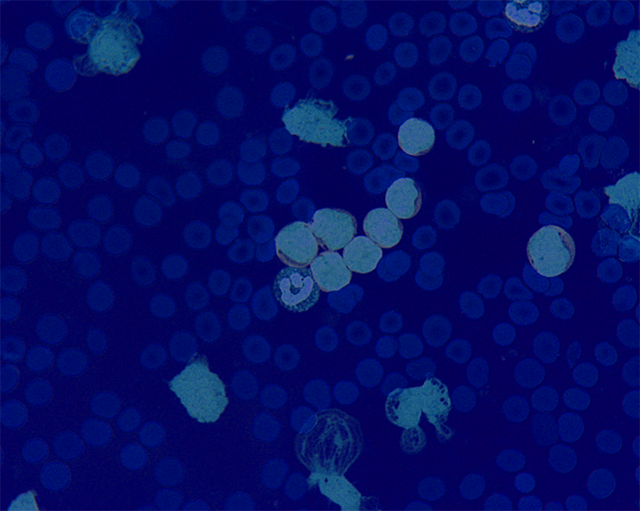
\includegraphics[width=0.3\textwidth]{images/figcs_cmyk124}
	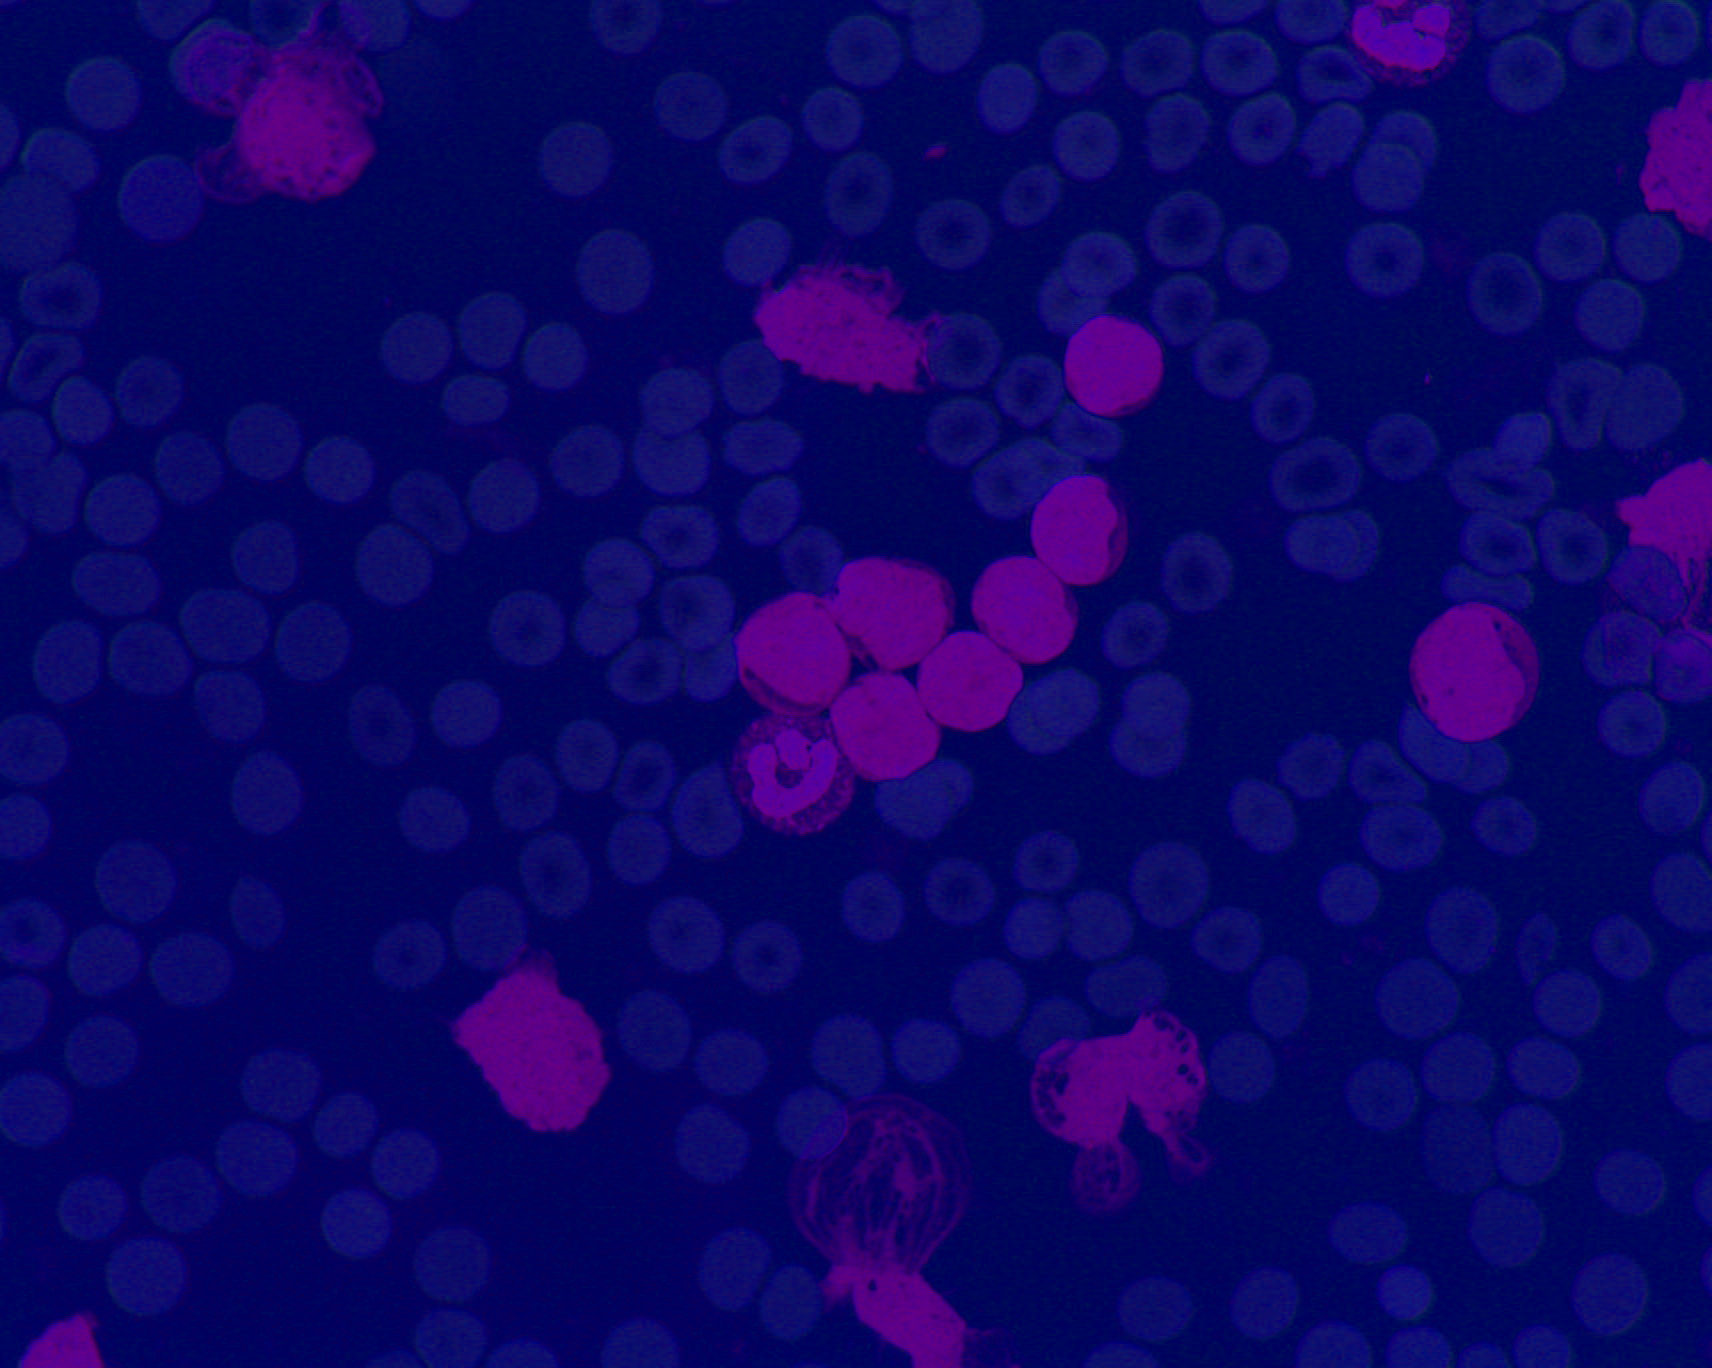
\includegraphics[width=0.3\textwidth]{images/figcs_cmyk234}
	\caption[Example of primary spaces.]{\label{fig:colour_spaces}Example of primary spaces image representation. From left to right and from top to bottom: RGB image, XYZ image, CYMK image; CMY image, CMK image, MYK image.}
\end{figure}

\pagebreak

\subsection{Luminance-Chrominance Spaces}  % DONE
The luminance-chrominance spaces are used if it is useful to separate the color definition into luminance, represented by one component, and chrominance, represented by the two other components. Among these color spaces, there are the television transmission color spaces, sometimes known as transmission primaries, YIQ, and YUV for analogical standard and YCbCr for the digital standard. For this reason, only the YCbCr has been taken into account. It could be obtained from the RGB color space using the following equation:

\begin{equation}\label{Ycbcr}
\left [ {  \begin{array}{c} Y  \\ Cb   \\ Cr \end{array} } \right ] = \left [{ \begin{array}{c} 0  \\ 128   \\ 128  \end{array} } \right ] +
\left [ { \begin{array}{c c c} \mbox{ 0.299}  & \mbox{ 0.587} & \mbox{ 0.114 } \\ \mbox{-0169} & \mbox{-0.331} & \mbox{ 0.500 } \\ \mbox{ 0.500} & \mbox{-0.419} & \mbox{-0.081 }  \end{array} } \right ] \cdot \left [ { \begin{array}{c} R  \\ G  \\ B  \end{array} } \right ] 
\end{equation}
\\
The International Commission of Illumination (CIE) has defined a system that classifies color according to the human visual system in order to specify any color in terms of its CIE coordinates. There are two main CIE based color spaces, CIELUV (Luv) and CIELAB (Lab). They are nearly linear with visual perception with the L parameter that has a good correlation with perceived lightness and the other two parameters that express the chrominance. Fig. \ref{fig:colour_spaces_lum} shows some examples. They are based on the XYZ color space so they could be obtained by a conversion from the XYZ color space using the following equations:

\textit{Luv}
\begin{equation} \label{Luv}
\begin{split}
&L = \begin{cases} 116 \sqrt[3]{y_r} -16, & y_r > 0.008856 \\ 903.3y_r, & y_r \leq 0.008856 \end{cases} \\
&u = 13L \left ( u' - u'_r \right)\\
&v = 13L \left ( v' - v'_r \right)
\end{split}
\end{equation}

where

\begin{equation*}
\begin{split}
&y_r = \frac{Y}{Y_r}\\
&u' = \frac{4X}{X + 15Y + 3Z}\\
&v' = \frac{9Y}{X + 15Y + 3Z}\\
&u'_r= \frac{4X_r}{X_r + 15Y_r + 3Z_r}\\
&v'_r = \frac{9Y_r}{X_r + 15Y_r + 3Z_r}
\end{split}
\end{equation*}

\textit{Lab}
\begin{equation} \label{Lab}
\begin{split}
&L = 116 \cdot h \left ( \frac{Y}{Y_r} \right ) -16\\
&a = 500 \left [ h \left ( \frac{X}{X_r} \right ) \left ( \frac{Y}{Y_r}  \right)  \right ]\\
&b = 200 \left [ h \left ( \frac{Y}{Y_r} \right ) \left ( \frac{Z}{Z_r}  \right)  \right ]
\end{split}
\end{equation}

where

\begin{equation*}
h(q) = \begin{cases} \sqrt[3]{q}, & q >0.008856 \\ 7.787q + 16/116, & q \leq 0.008856 \end{cases}
\end{equation*}

\noindent Both equations require a reference white $X_r$, $Y_r$ and $Z_r$.

\begin{figure}[!h]
	\centering
	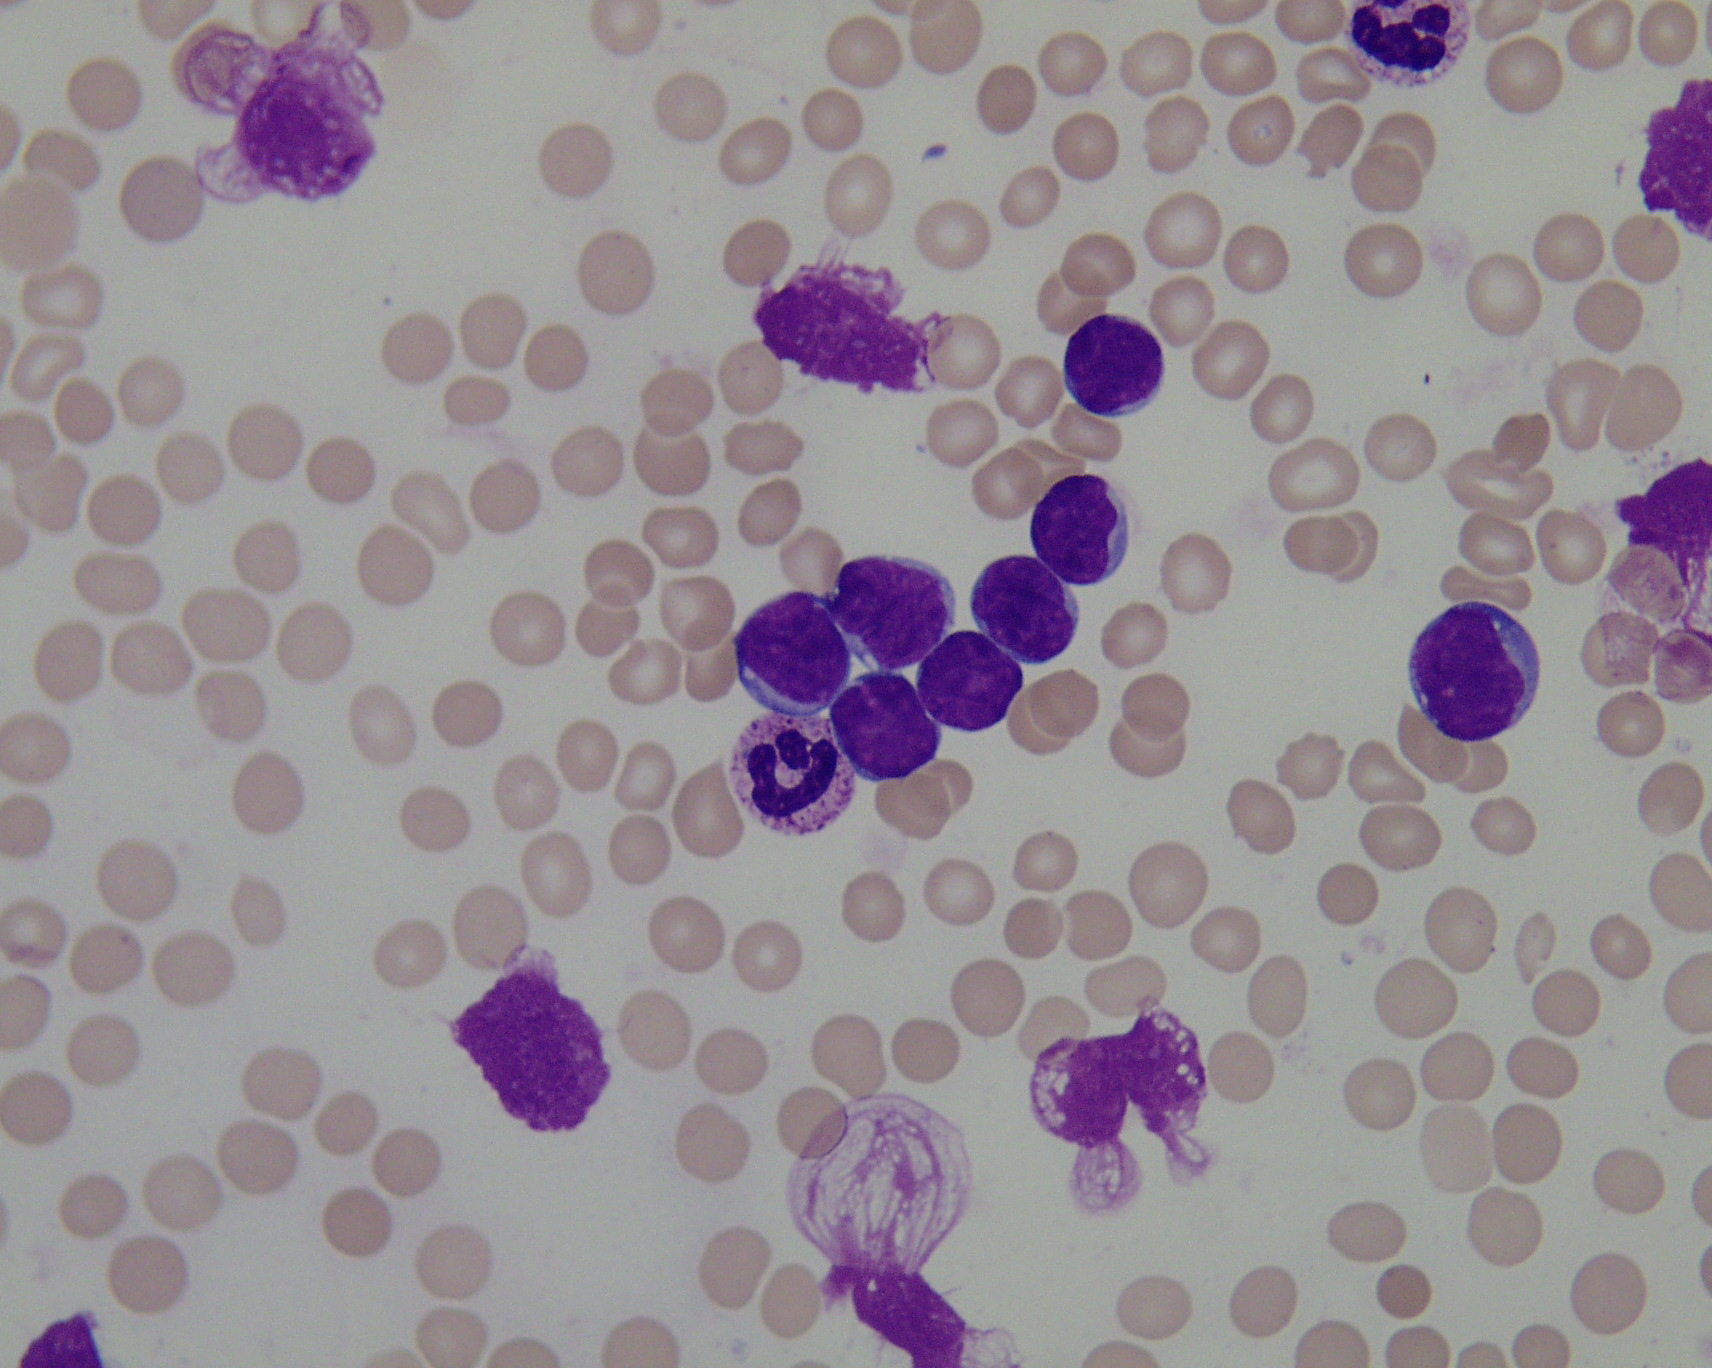
\includegraphics[width=0.25\textwidth]{images/figcs_rgb}
	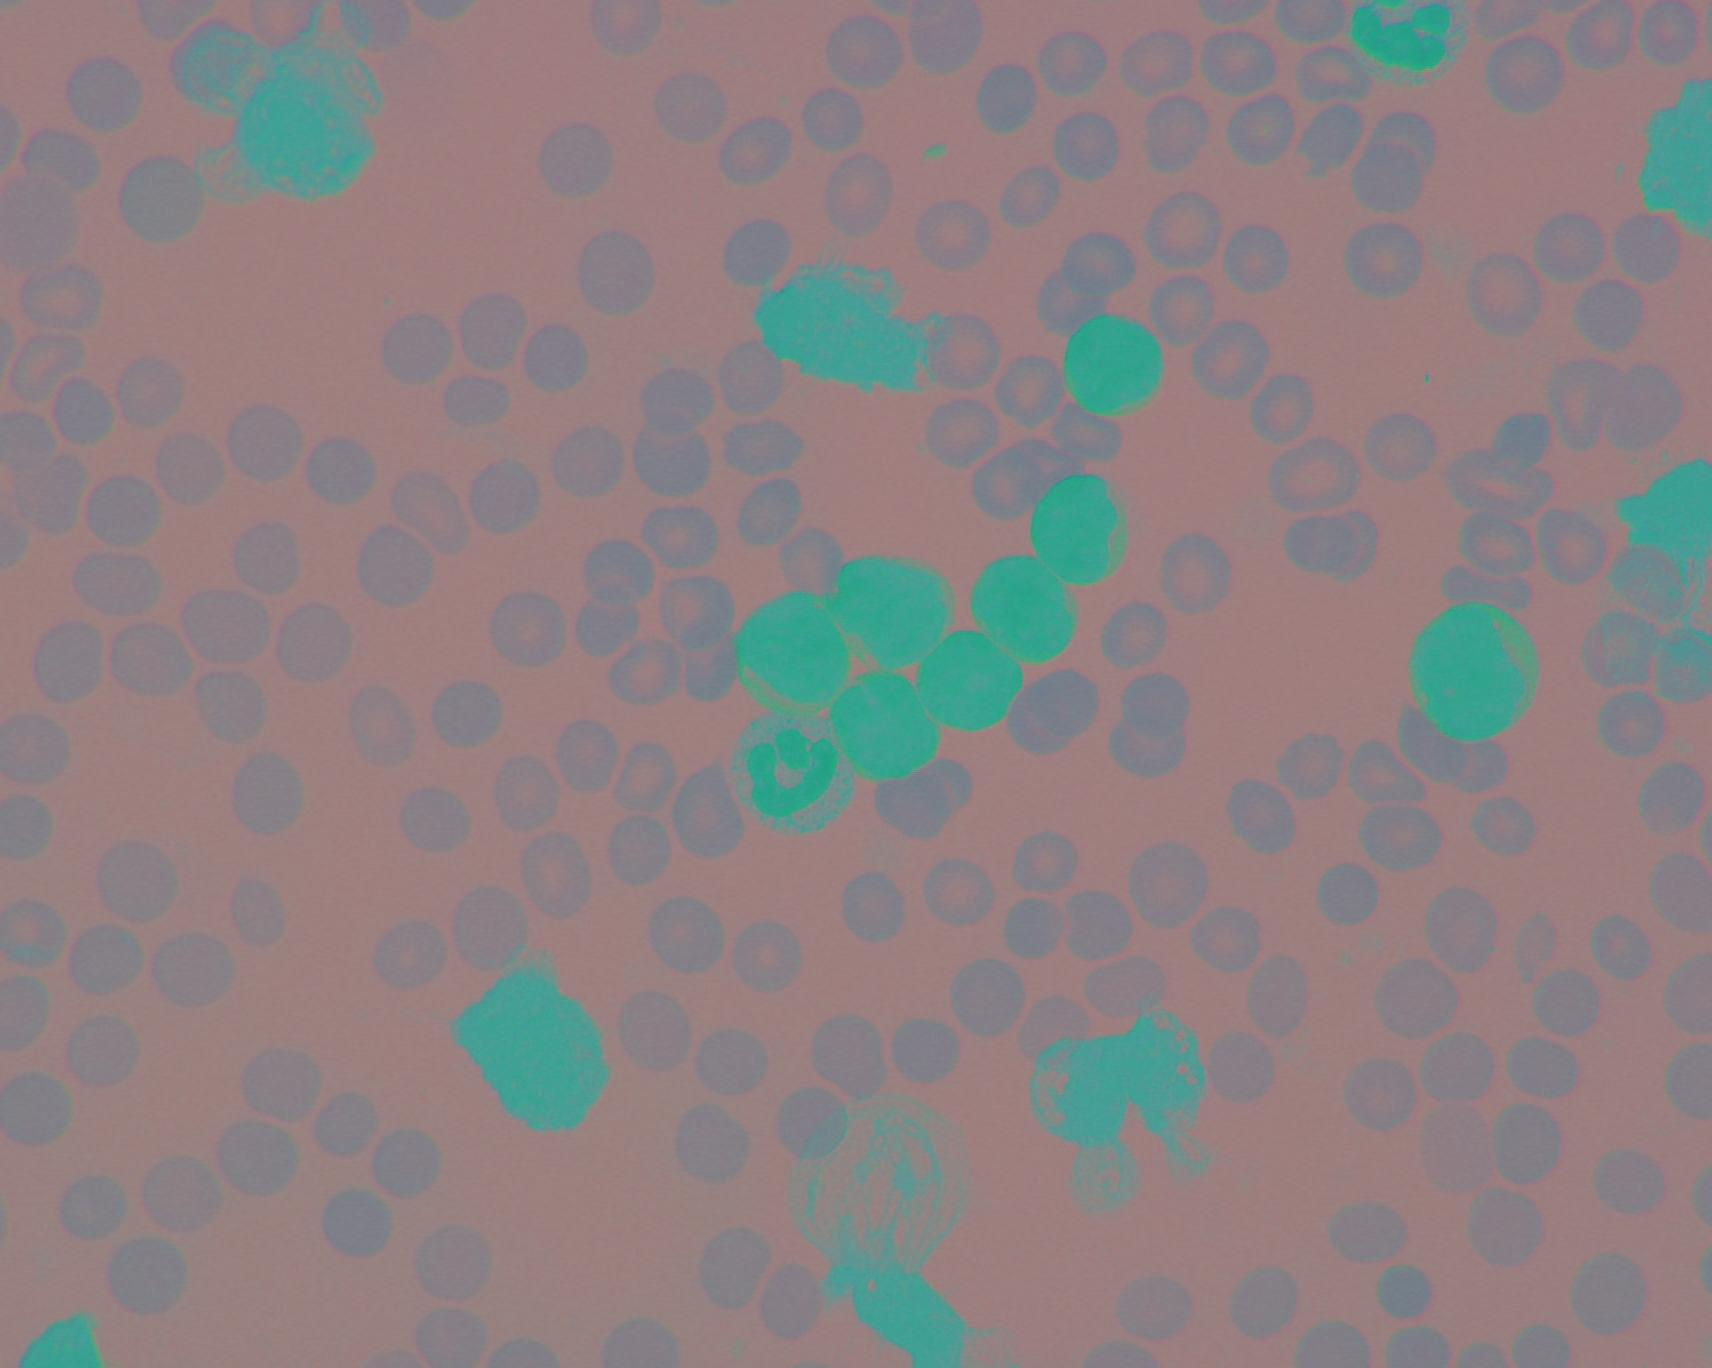
\includegraphics[width=0.25\textwidth]{images/figcs_ycbcr}
	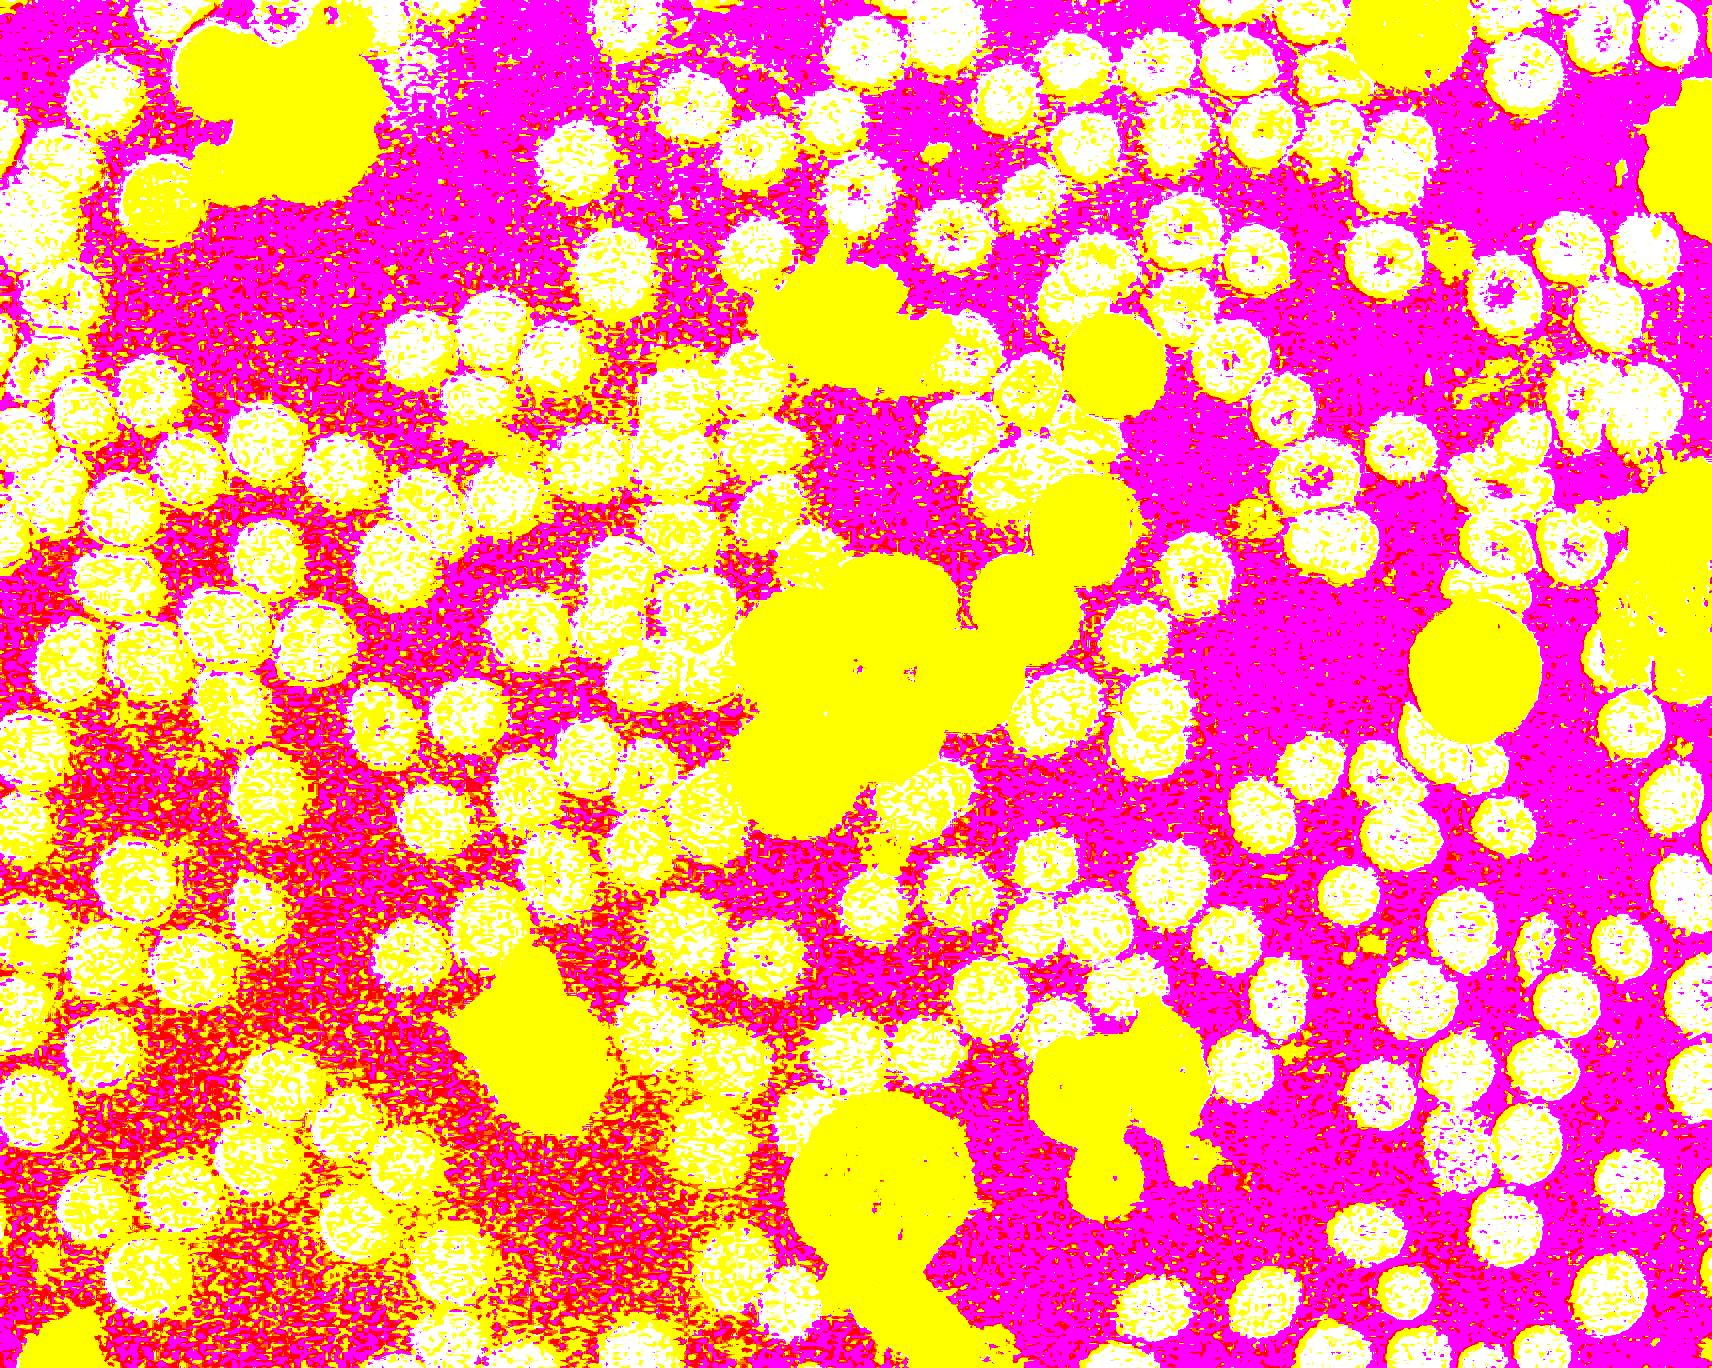
\includegraphics[width=0.25\textwidth]{images/figcs_lab}
	\caption[Example of Luminance-Chrominance spaces.]{\label{fig:colour_spaces_lum}Example of Luminance-Chrominance spaces. From left to right: RGB, Ycbcr and Lab images.}
\end{figure}


\subsection{Perceptual Spaces}  % DONE
The perceptual spaces try to quantify the subjective human color perception through Intensity, Hue and Saturation values. This family represents a wealth of similar color spaces, which include HSI (I stands for Intensity), HSV (V stands for Value), HSL (Hue Saturation Lightness), HCI (C stands for Chroma), and so on. Most of these color spaces are linear transforms from RGB and, consequently, are device dependent. Fig. \ref{fig:colour_spaces_per} depicts some examples. Their advantage lies in the extremely intuitive manner of specifying color, selecting the desired hue and then modifying it slightly by adjusting its saturation and intensity values.
Furthermore, the separation of the luminance component from color information is stated to have advantages in image processing. Here only the HSV color space has been taken into account since it is the most used perceptual space. It can be obtained from the RGB color space with the following equation:

\begin{equation}\label{HSV}
\begin{split}
&Max = max(R, G, B)\\
&Min = min(R, G, B)\\
&\Delta = Max-Min\\
&V = Max\\
&S = \frac{(\Delta)}{Max}\\
&H = \begin{cases} 0, & \mbox{if   } \Delta = 0 \\ 60^\circ \times \left (\frac{G-B}{\Delta} mod6 \right ), & \mbox{if   } R = Max \\  
60^\circ \times \left ( \frac{B-R}{\Delta} + 2 \right ), & \mbox{if   } G = Max\\ 
60^\circ \times \left ( \frac{R-G}{\Delta} + 4 \right ), & \mbox{if   } B = Max\end{cases} 
\end{split}
\end{equation}

\begin{figure}[h]
	\centering
	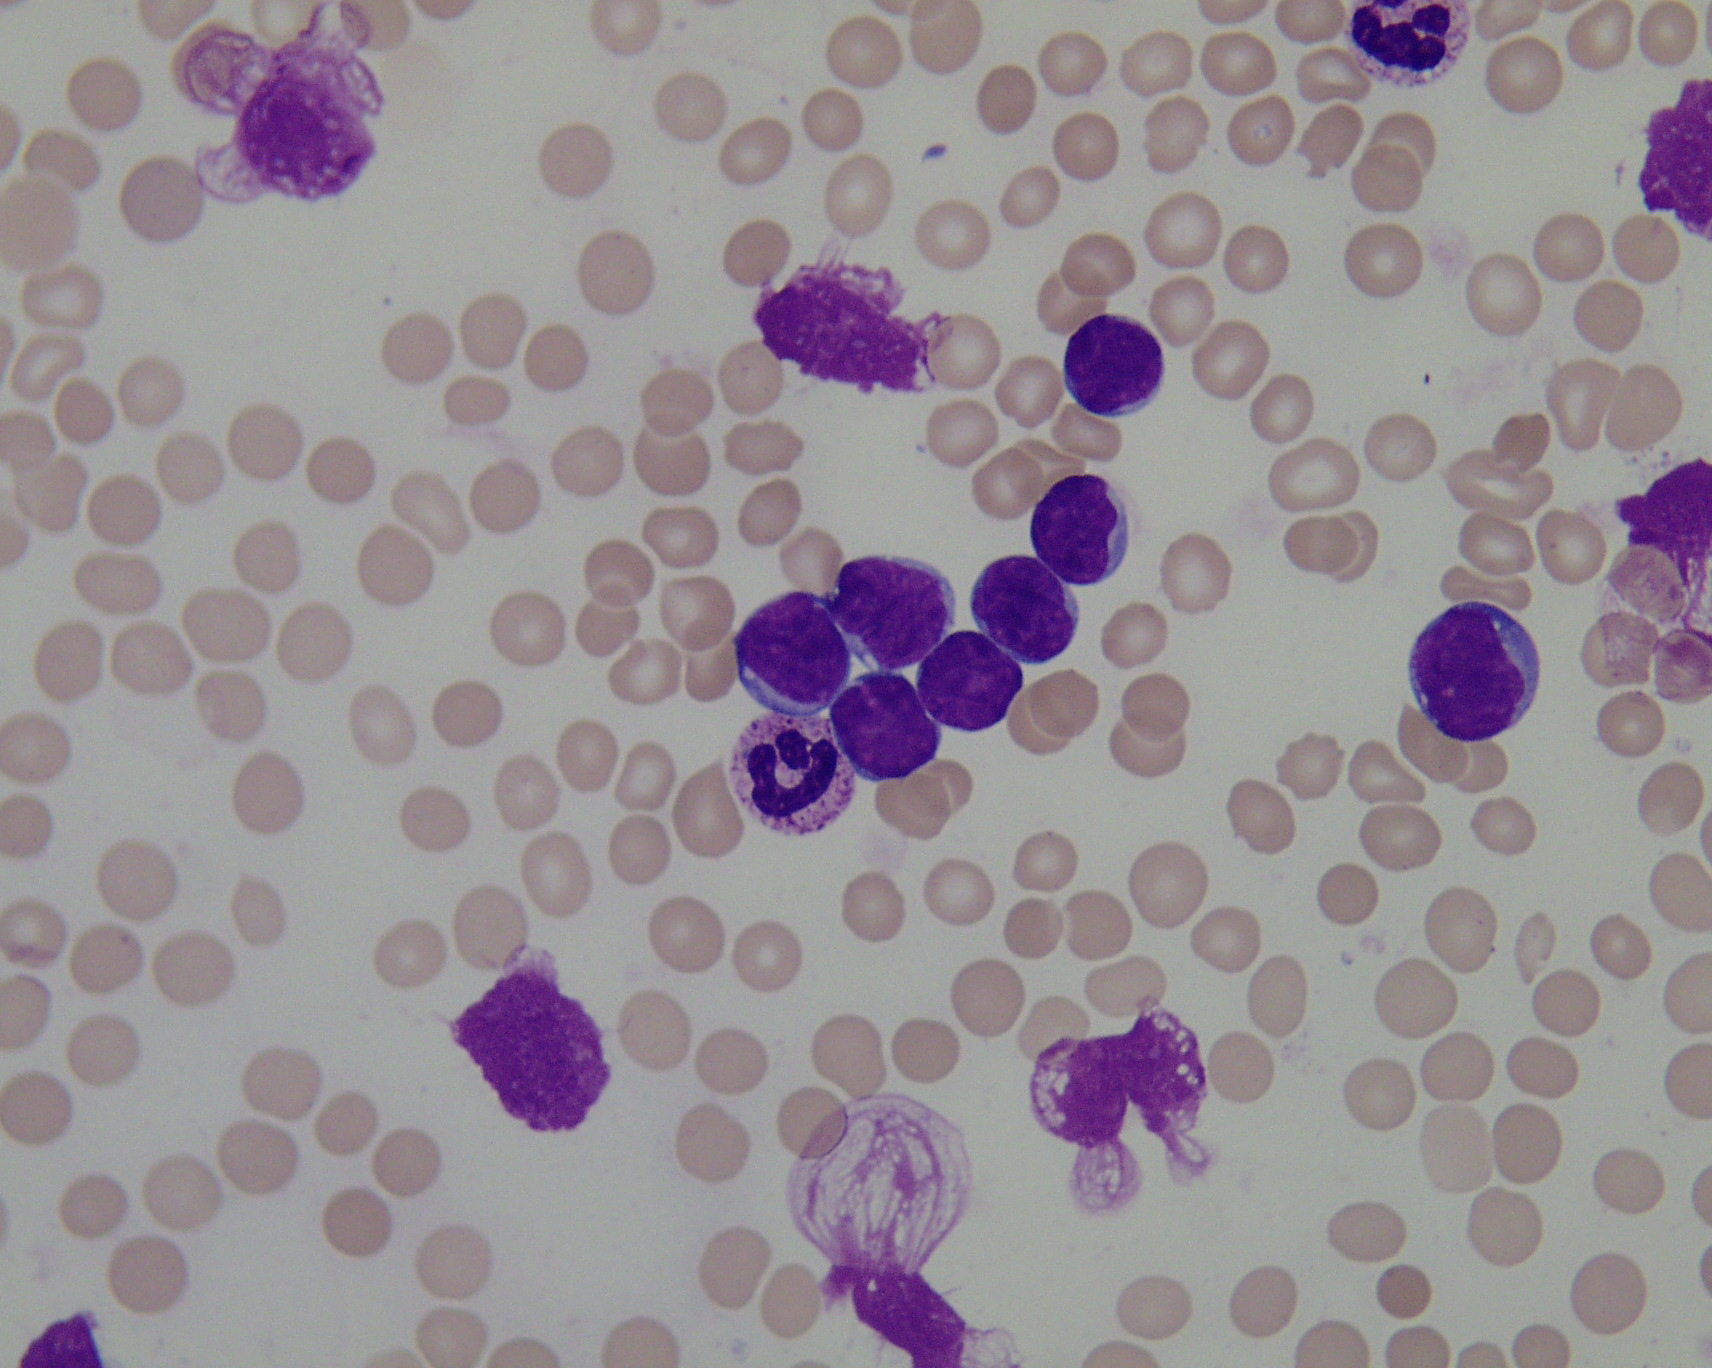
\includegraphics[width=0.25\textwidth]{images/figcs_rgb}
	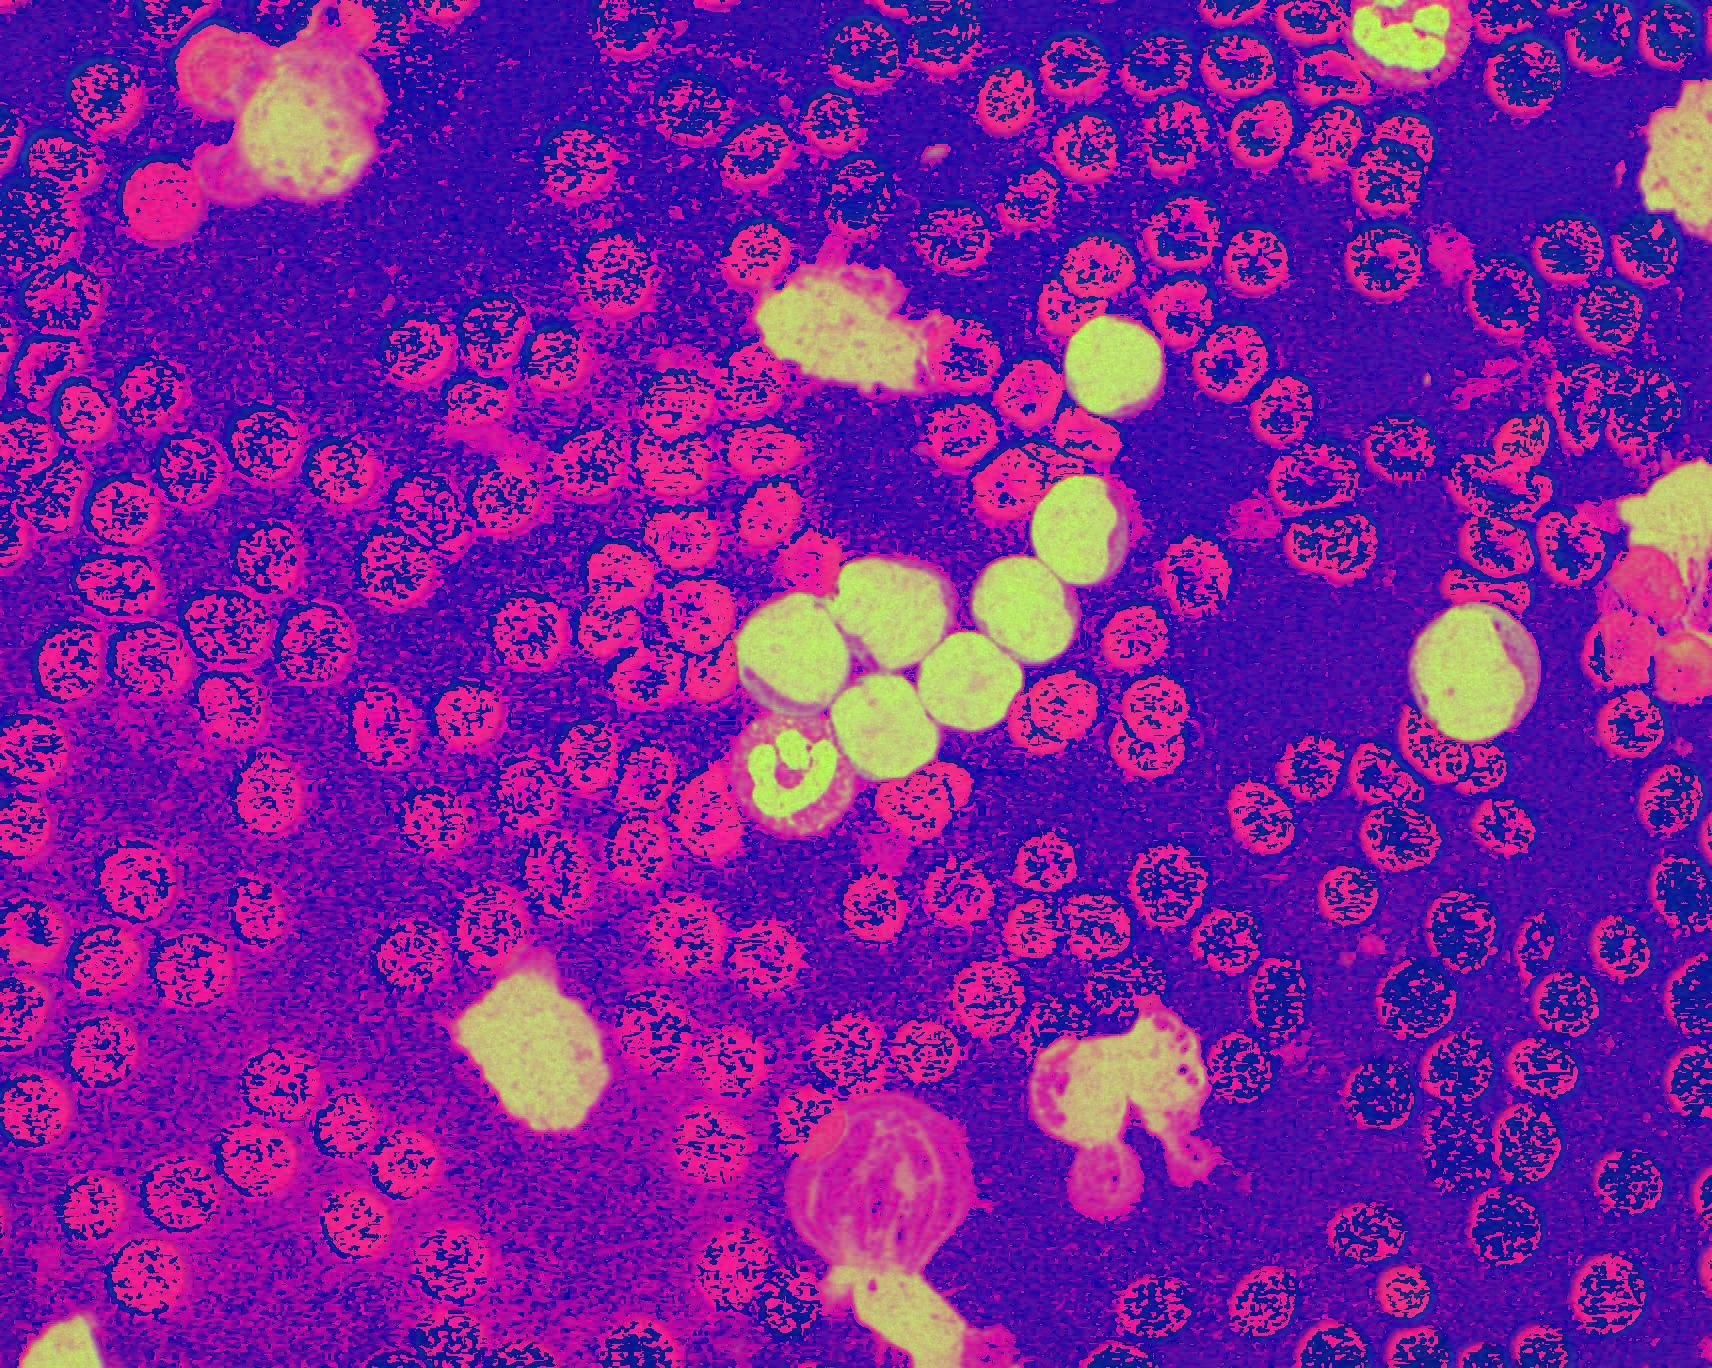
\includegraphics[width=0.25\textwidth]{images/figcs_hsv}
	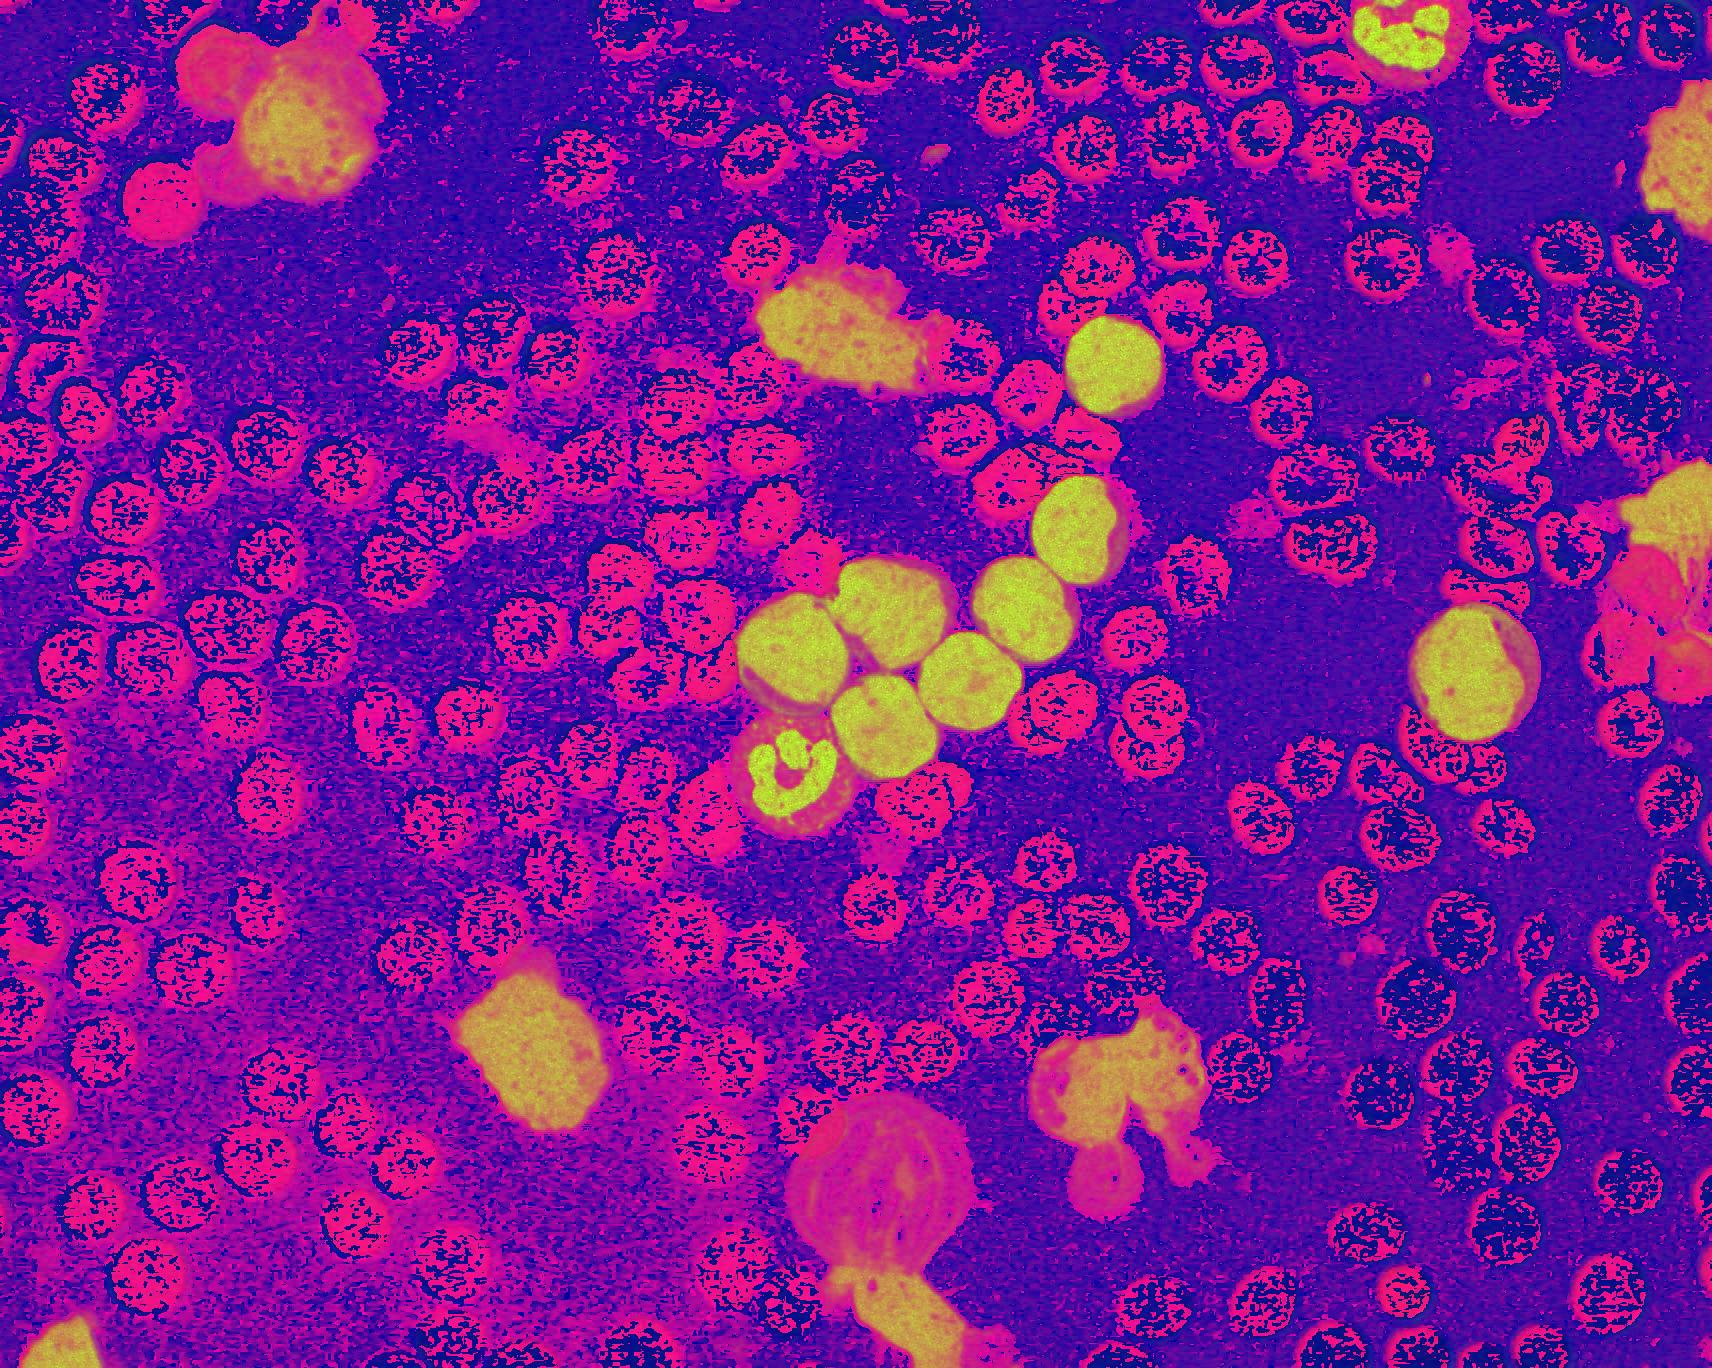
\includegraphics[width=0.25\textwidth]{images/figcs_hsl}
	\caption[Example of perceptual spaces.]{\label{fig:colour_spaces_per}Example of perceptual spaces. From left to right: RGB, HSV, HSL images.}
\end{figure}

\chapter{Segmentation}
Segmentation is one of the most important steps in image analysis because it permits to identify and separate, according to specific criteria of homogeneity and separation, the different regions contained in the image. Its main objective is to divide the image into parts that have a strong correlation either between them or with objects and areas of the real world contained in the image. The commonly used segmentation methods operate essentially relying on characteristics such as the value of brightness, color, and reflection of the individual pixels, identifying groups of pixels that correspond to spatially connected regions. 
As for many problems of image processing, no standard solution exist in general. Therefore, depending on the characteristics of the images to process, and especially of the objects to be segmented, different segmentation techniques can be applied. The simplest can often lead to unsatisfactory results, while the remaining are more powerful, but their drawback is a higher computational cost. For medical images analysis, two primary levels of segmentation exist: the first level aims to separate whole cells from the background and the second one seeks to separate the cells in their components like the nucleus from the cytoplasm in WBCs analysis or intracellular parasites in RBCs analysis, for example. The second segmentation level is quite common in cells analysis because the cell class depends on the morphological characteristics of its components. The segmentation techniques can be divided into three main categories: Pixel-Based, Edge-Based and Region Based.

\section{Pixel Based or Thresholding} % DONE
Thresholding is the most elementary and computationally cheaper technique for image segmentation, making use of a threshold operator that directly involves the image histogram. The hypothesis underlying this segmentation technique is that the pixels of an object approximately have the same brightness and, therefore, they can be separated from the background by thresholding brightness values. The problem becomes more difficult if the histogram presents more than two peaks because more than one threshold value is necessary to separate the image objects. This technique presents some drawbacks, in particular, if the threshold is not chosen accurately, the detected objects can shrink or grow. This change in size can be crucial in applications where size is an essential parameter for the classification of the object itself.
Moreover, an incorrect threshold value can cause a partial fusion of two or more objects together, making it impossible to perform its subsequent classification and identification. When the intensity distribution of objects and background is sufficiently distinct, it is possible to use a single global threshold \cite{Gonz, GonzMAT} applicable to the entire image. The value of this global threshold is calculated starting from an initial threshold value $T$ between the minimum and maximum value of the histogram, that allows making the first segmentation. It produces two groups of pixels. Their values are averaged and used to calculate the new threshold value $T$. The process is then iterated until the difference between successive values of $T$ is less than a predetermined parameter. This simple algorithm works well in situations where there is a clear valley between the various fashions histogram, relative to the background and objects.

\begin{figure}[h]
	\centering
	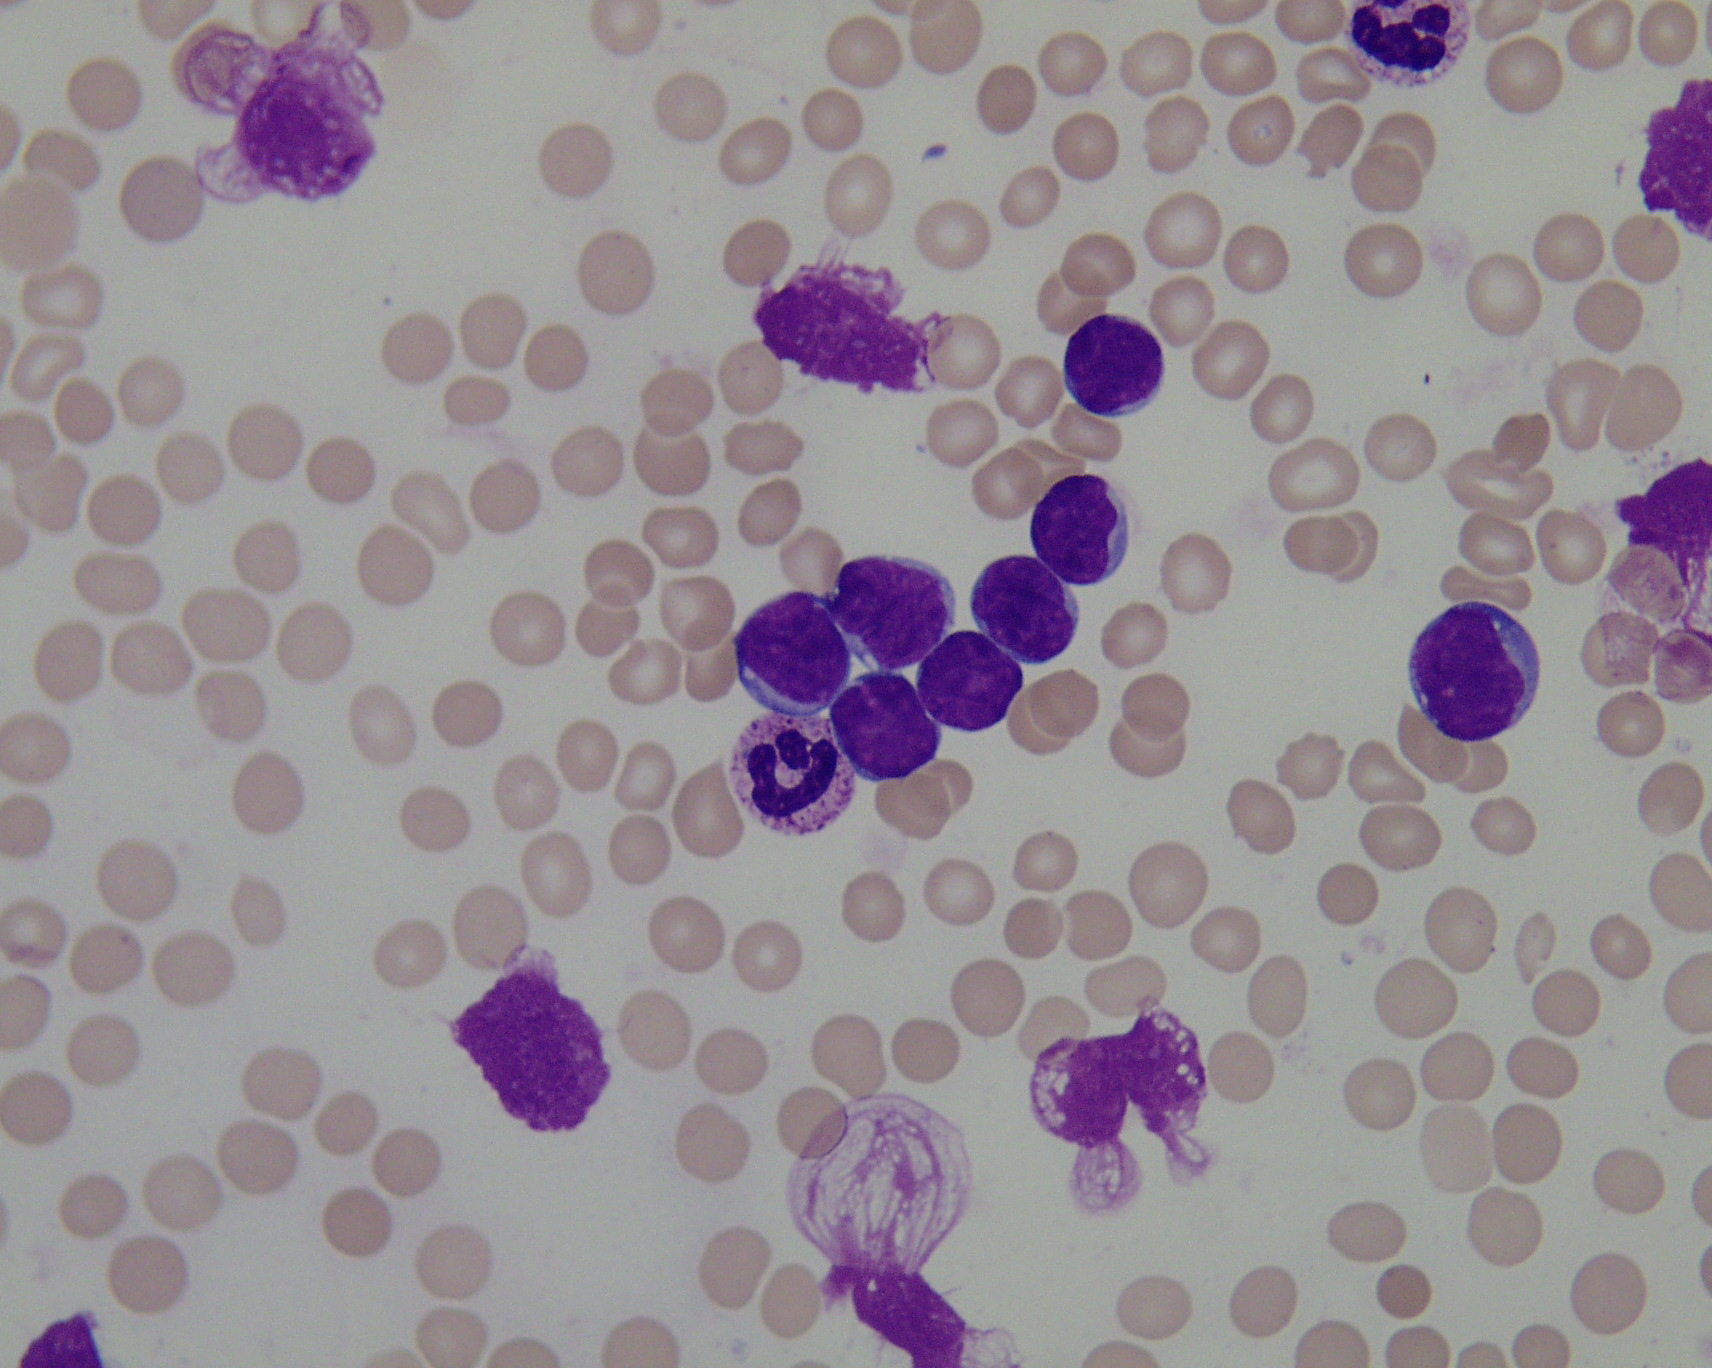
\includegraphics[width=0.3\textwidth]{images/figcs_rgb}
	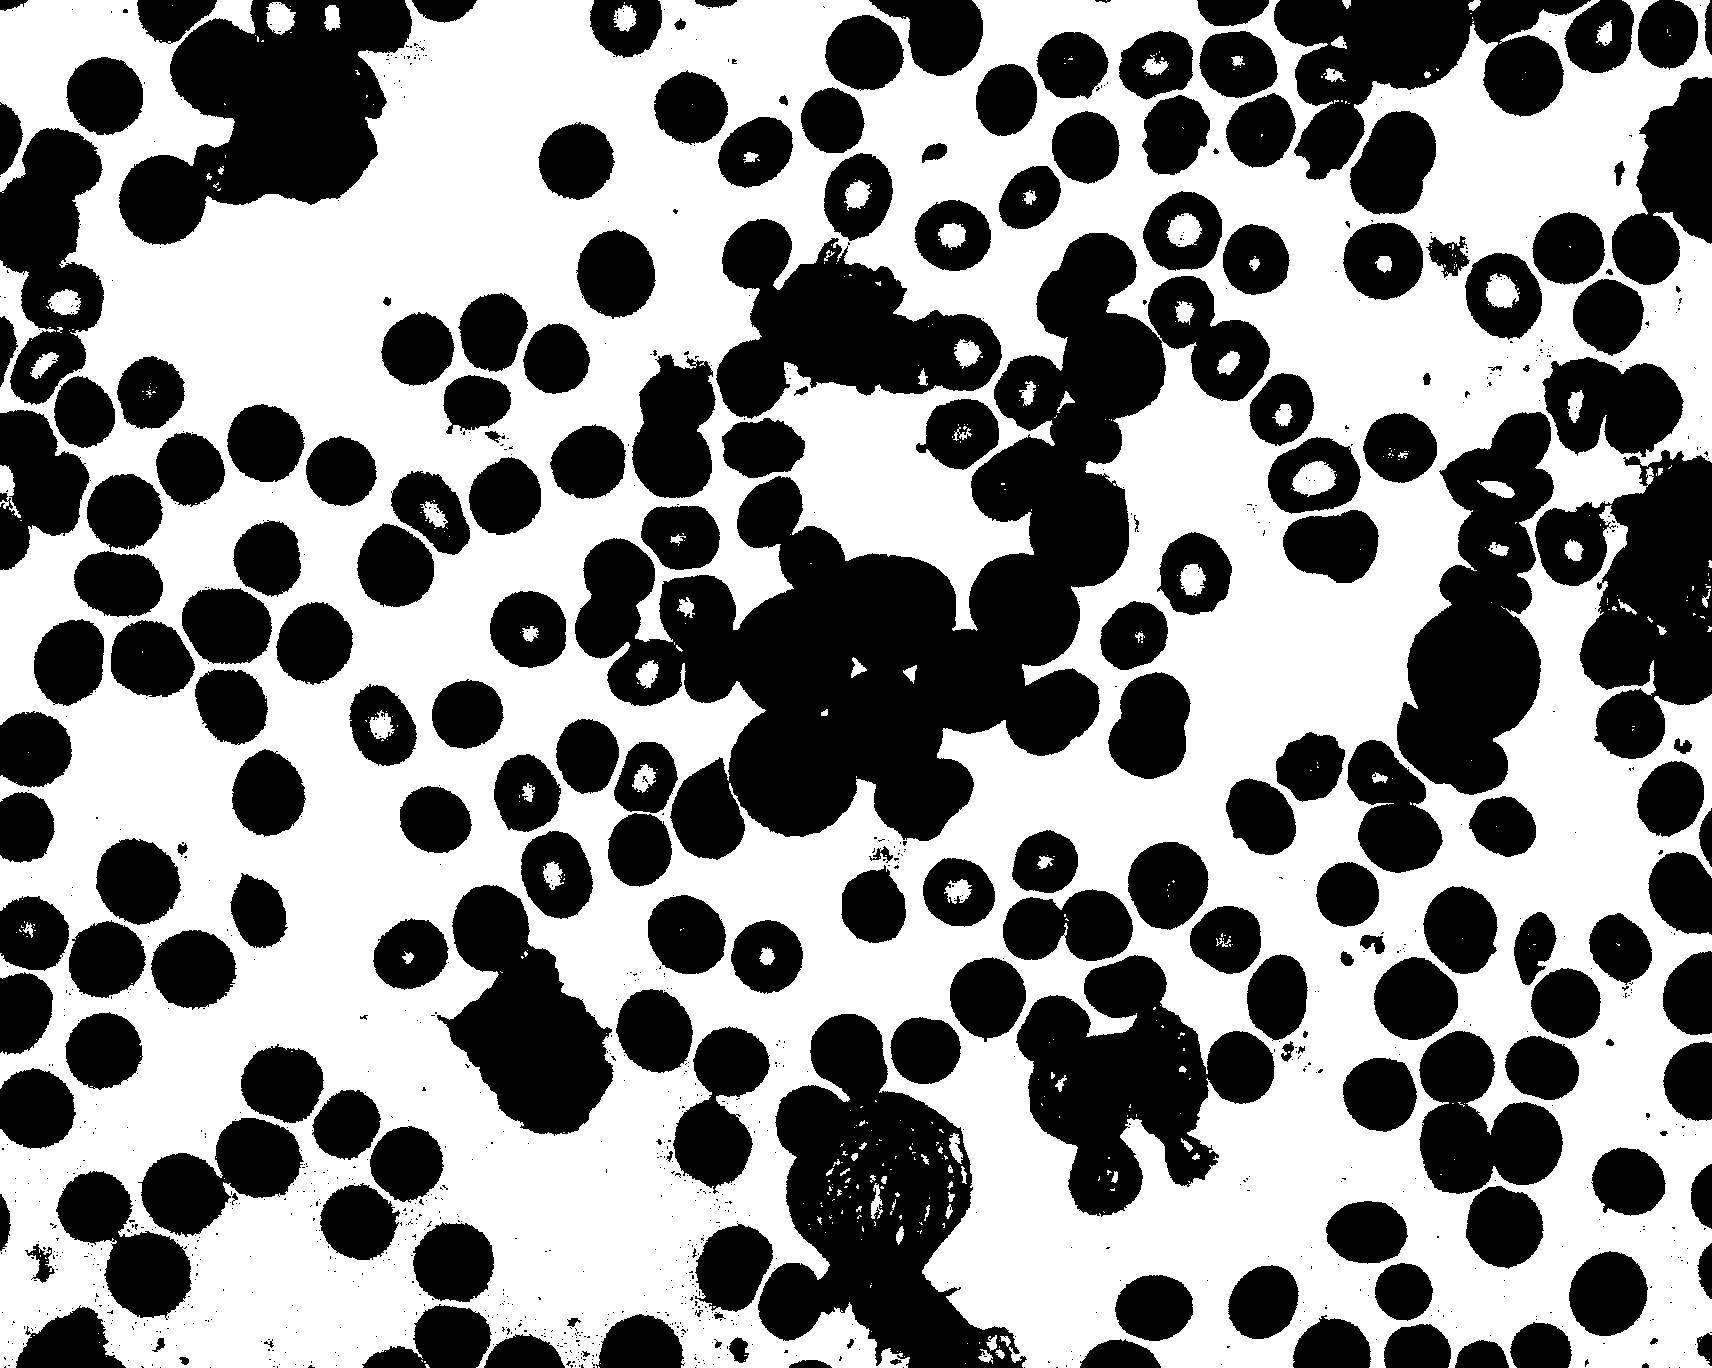
\includegraphics[width=0.3\textwidth]{images/fig_global}
	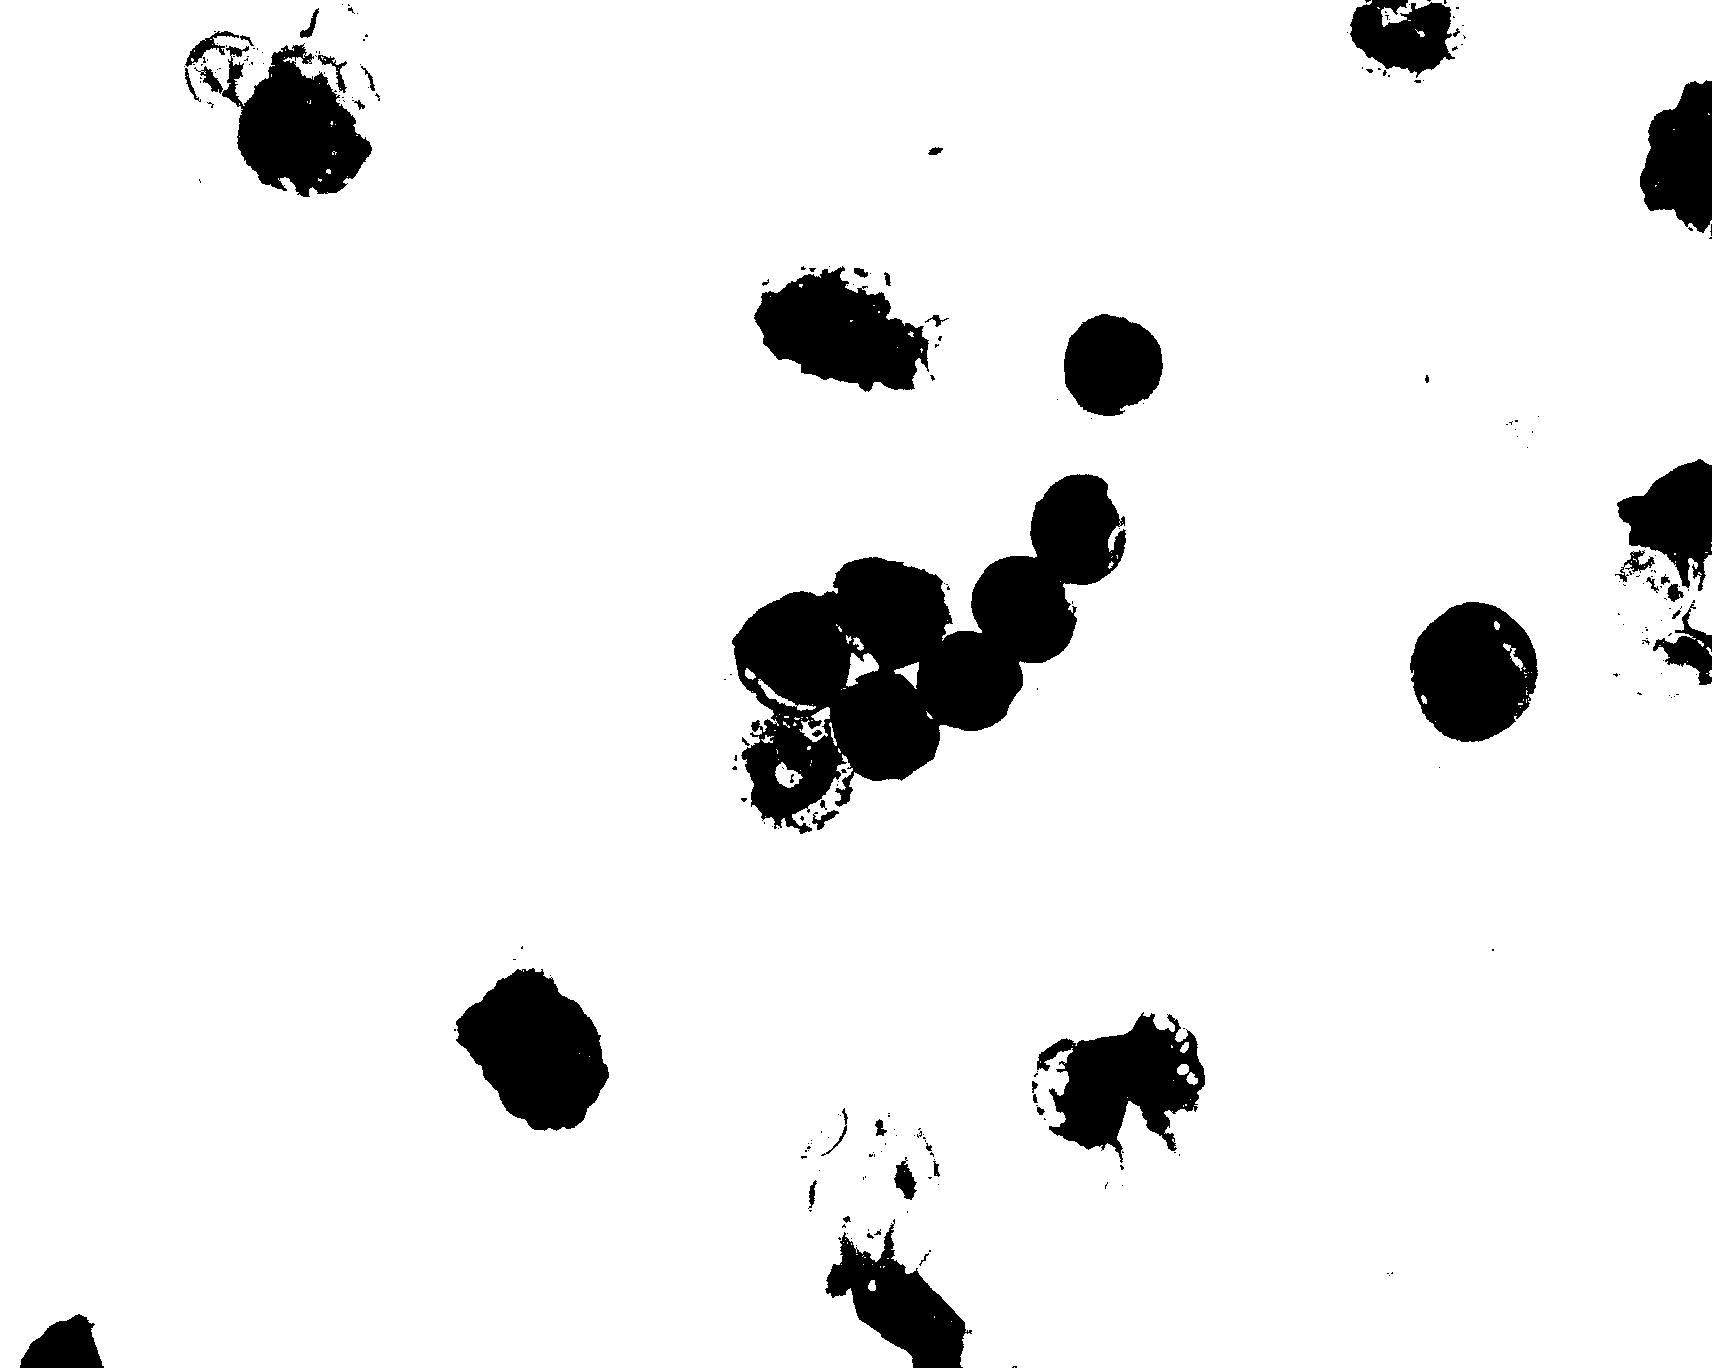
\includegraphics[width=0.3\textwidth]{images/fig_otsu}
	\caption[Example of global thresholding.]{\label{fig:otsu}Example of global thresholding. From left to right: RGB original image, binary image resulting from a 0.6 global threshold value, binary image after Otsu threshold, which produced an optimal global threshold value of 0.4157.}
\end{figure}

\subsection{Otsu Algorithm} \label{Otsu} % DONE
The method of Otsu \cite{Otsu} also performs a global threshold, but differently from the previous one allows to obtain an optimal threshold value, as it maximizes the variance between classes, as shown in Fig. \ref{fig:otsu}. If well segmented, the classes are differentiated from the intensity value of their pixels. A threshold that gives the best separation between the classes in terms of intensity is an optimal threshold. The method of Otsu, moreover, can be extended to the segmentation of images that need more threshold values, since the measure of separability on which is based also extends to an arbitrary number of classes. It begins to lose meaning when the number of classes excessively increases since it works only with one variable which is the intensity. Typically, however, applications that require more than two threshold values are resolved with the use of other values in addition to the intensity, such as the color or the entropy present in the histogram \cite{Kapur}.

\subsection{Zack Algorithm} \label{Zack} % DONE
The Zack algorithm \cite{Zack}, also known as triangle method, differently from the other methods, does not work directly on the intensity value of the histogram, but it works on the image obtained from the histogram plot. It is called triangle method because it draws a sort of triangle, constructing a straight line that connects the highest histogram value $h[b_{max}]$ and the lowest one $h[b_{min}]$, where $b_{max}$ and $ b_{min}$ indicate the values of the grey levels where the histogram $h[x]$ reaches its maximum and minimum, respectively. The distance $d$ between the marked line and the histogram values between $b_{min}$ and $b_{max}$ is then calculated. The intensity value, where the distance $d$ reaches its maximum, defines the threshold value. This algorithm is particularly effective and fast, indeed, differently from the ones seen before, it is computed directly on an image without any further iteration.

\begin{figure}[h]
	\centering
	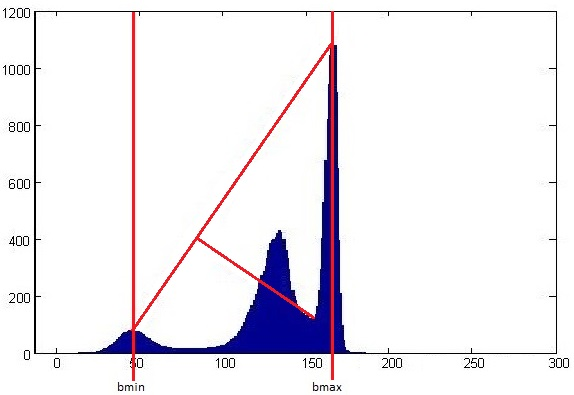
\includegraphics[width=0.57\textwidth]{images/Zack}
	\caption[Example of Zack algorithm.]{\label{fig:exampleZack}Example of Zack algorithm.}
\end{figure}

\subsection{Fuzzy Threshold} % DONE
The so far treated threshold algorithms are also called crisp techniques. They produce excellent results with sharp images and regions, but the segmentation process becomes complex in the presence of noise or imprecision. The nature of this imprecision in the image arises from the presence of uncertainty, that can lead to ill-defined regions. In this case, it is appropriate to avoid crisp segmentation and to prefer a fuzzy segmentation. Fuzzy threshold approaches are based on Fuzzy Sets (\acs{FS}s) theory. Regions may be viewed as fuzzy subsets of the image. Several researchers have worked on fuzzy based thresholding techniques, in particular, to identify the best fuzzy measure able to separate the fuzzy subset, such as the fuzzy compactness \cite{Pal}, the fuzzy similarity \cite{Ramar} or the fuzzy divergence and gamma membership \cite{Cha03, MeloP}.
Fuzzy threshold approaches segmentation performances are better than many crisp methods even though their computational performances are not comparable, as Fig. \ref{fig:fuzzy} shows. Crisp methods are entirely based on computations performed on the histogram, a 1-D array easily obtainable from the image, while fuzzy approaches are based on computations performed on the image, a 2-D array of size $M \times N$.

\begin{figure}[h]
	\centering
	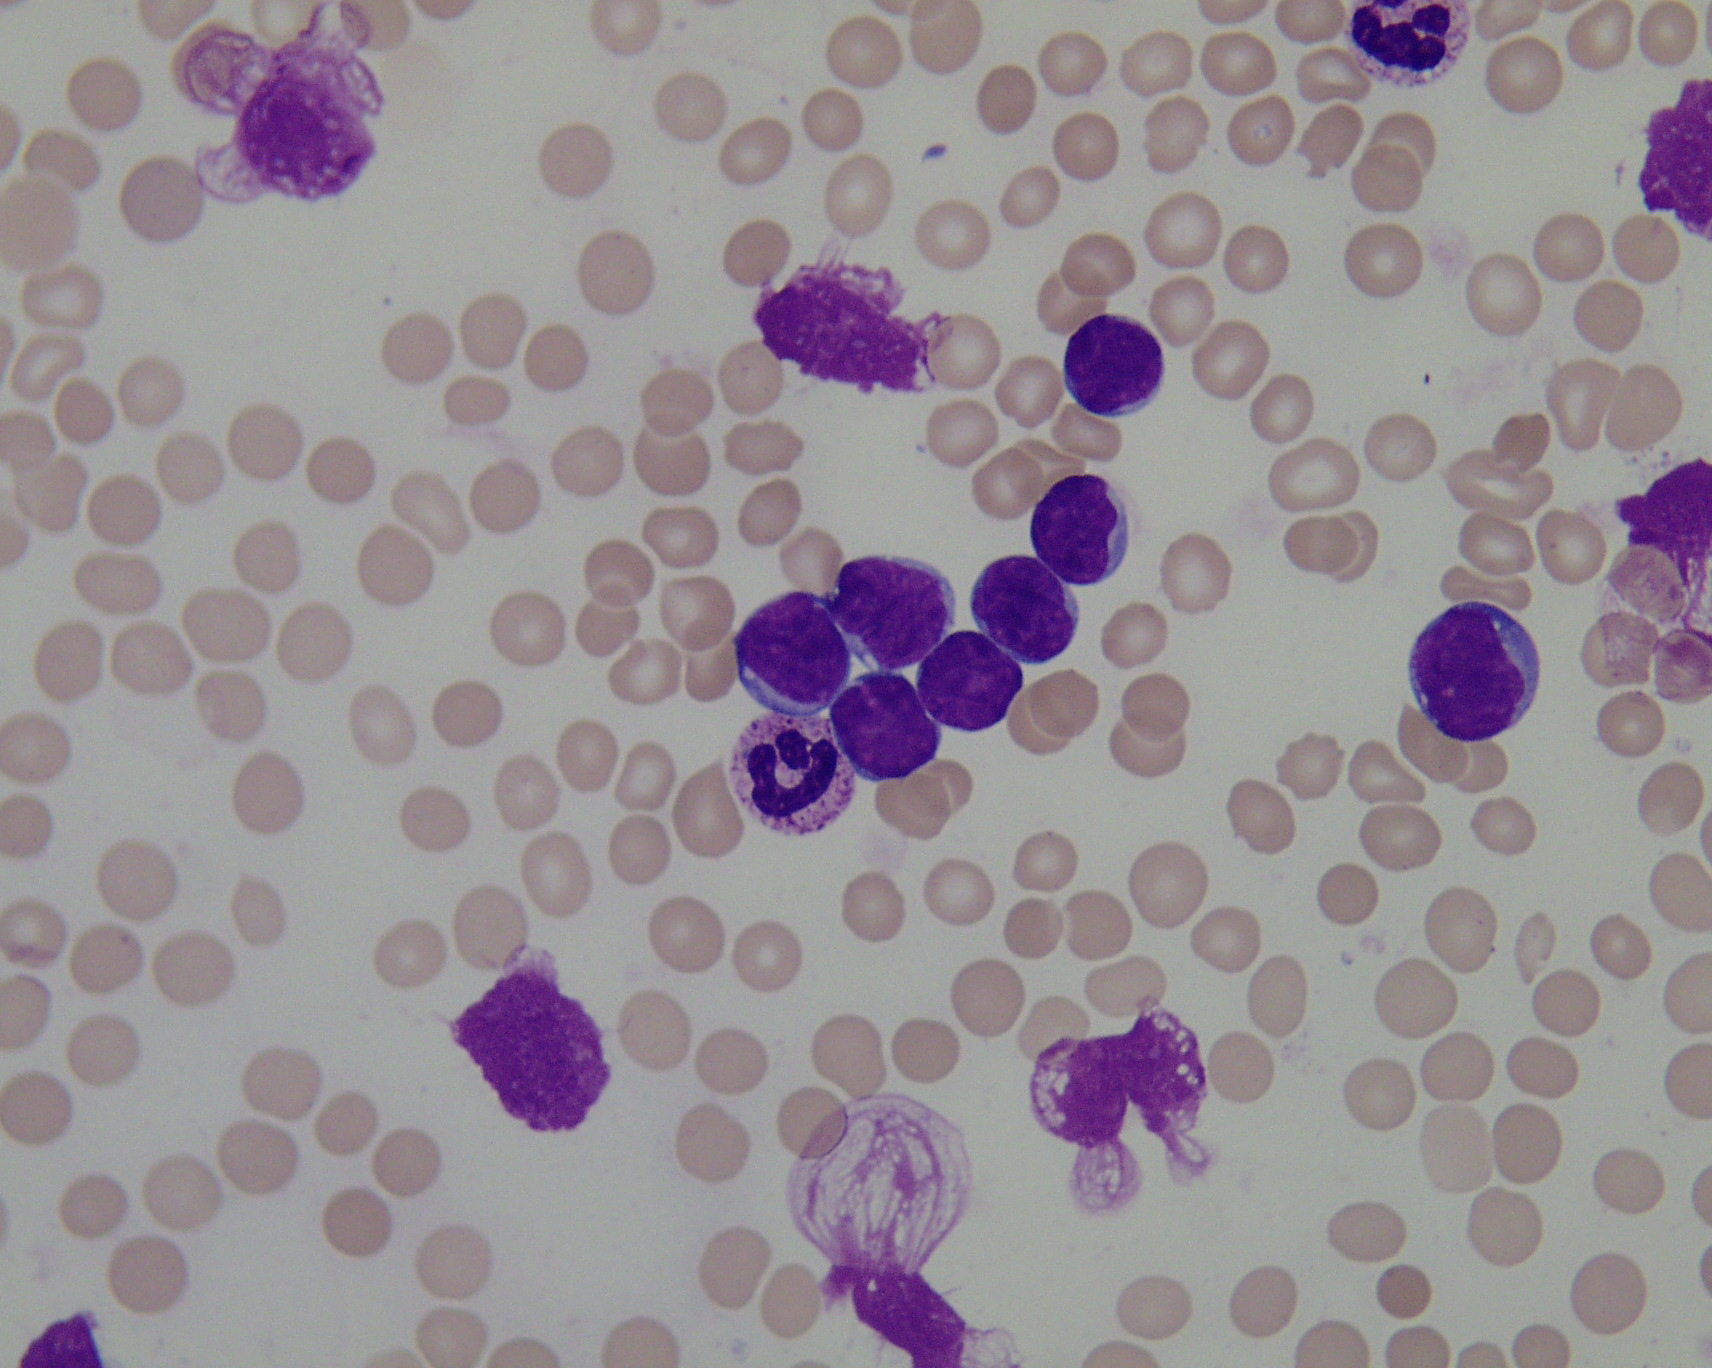
\includegraphics[width=0.3\textwidth]{images/figcs_rgb}
	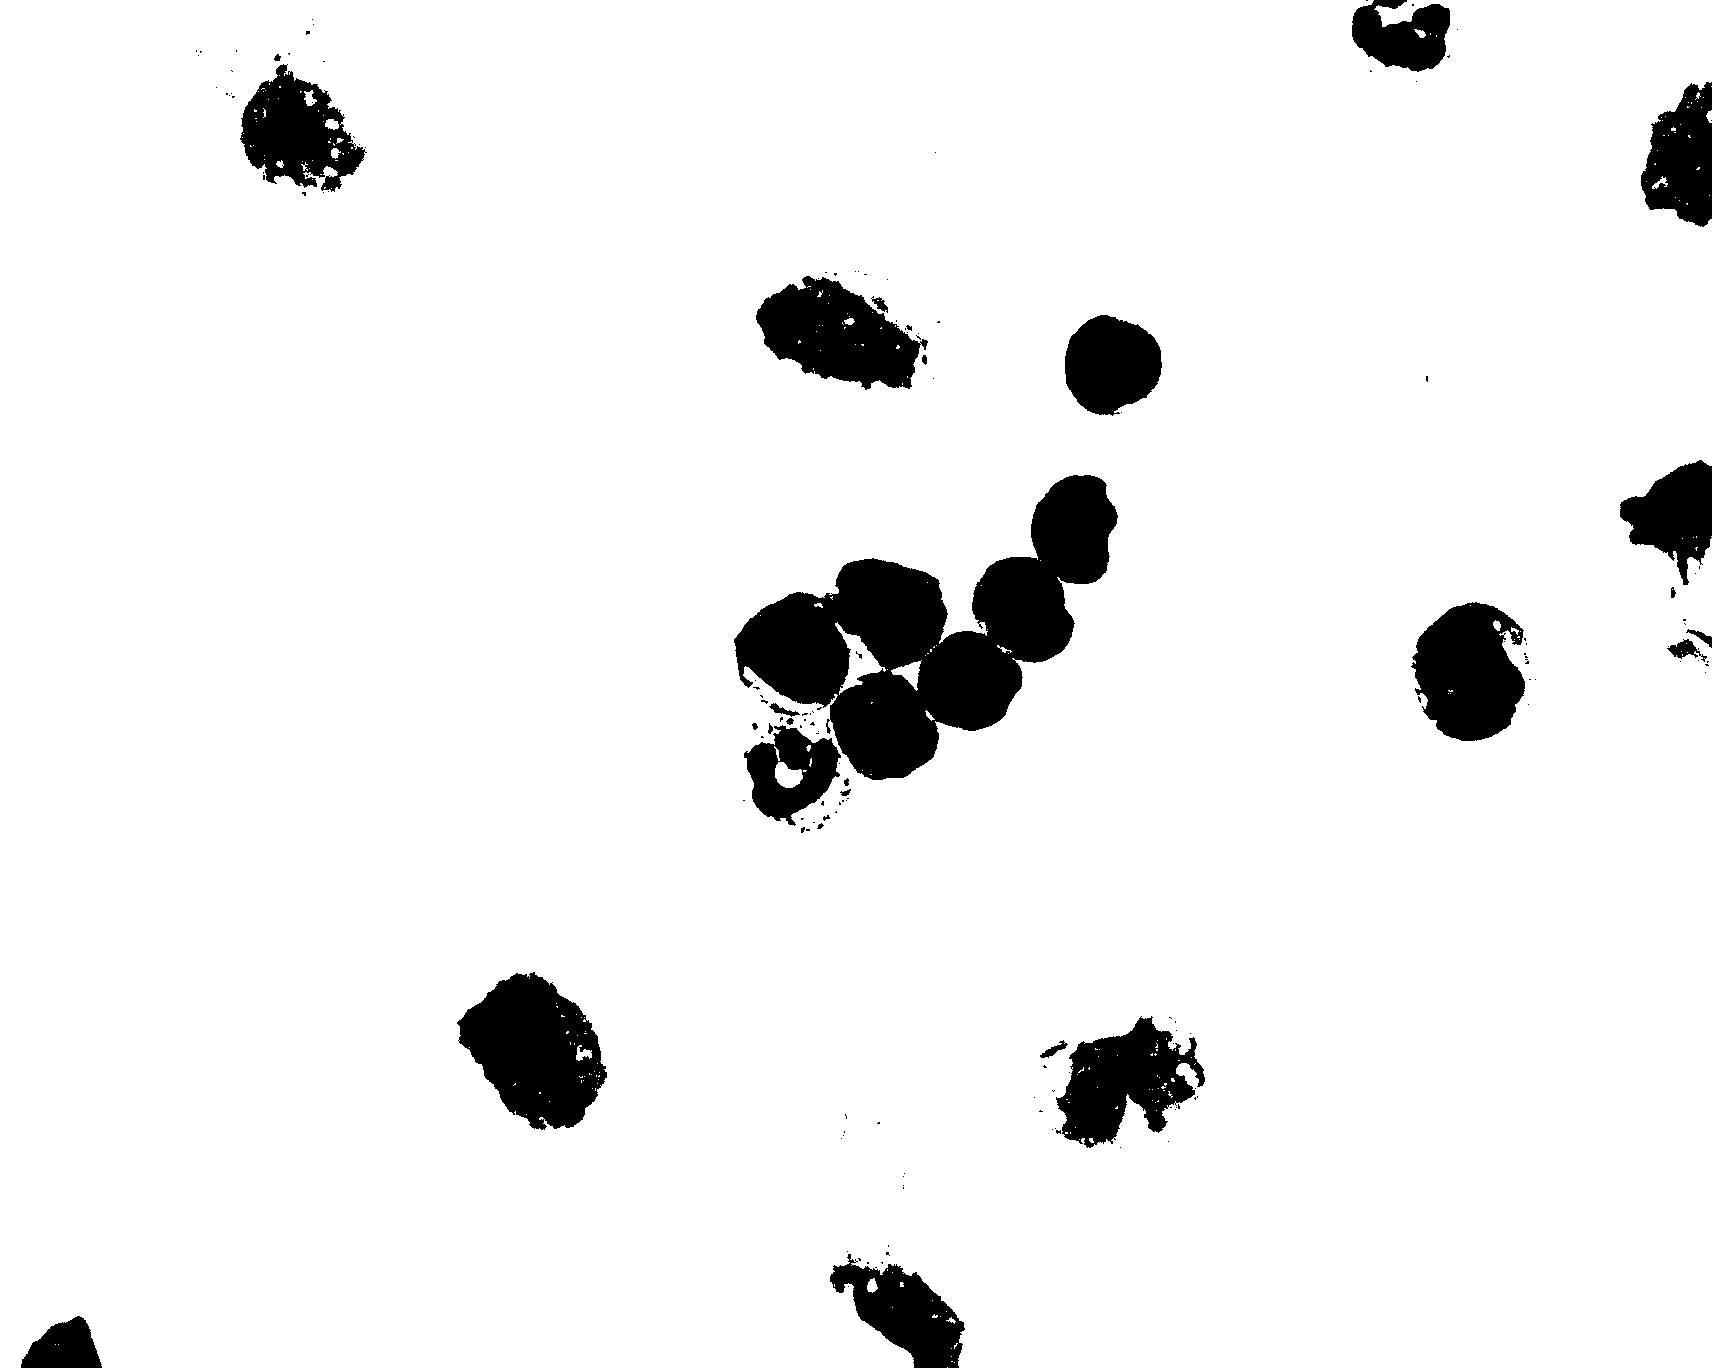
\includegraphics[width=0.3\textwidth]{images/fig_fuzzy1}
	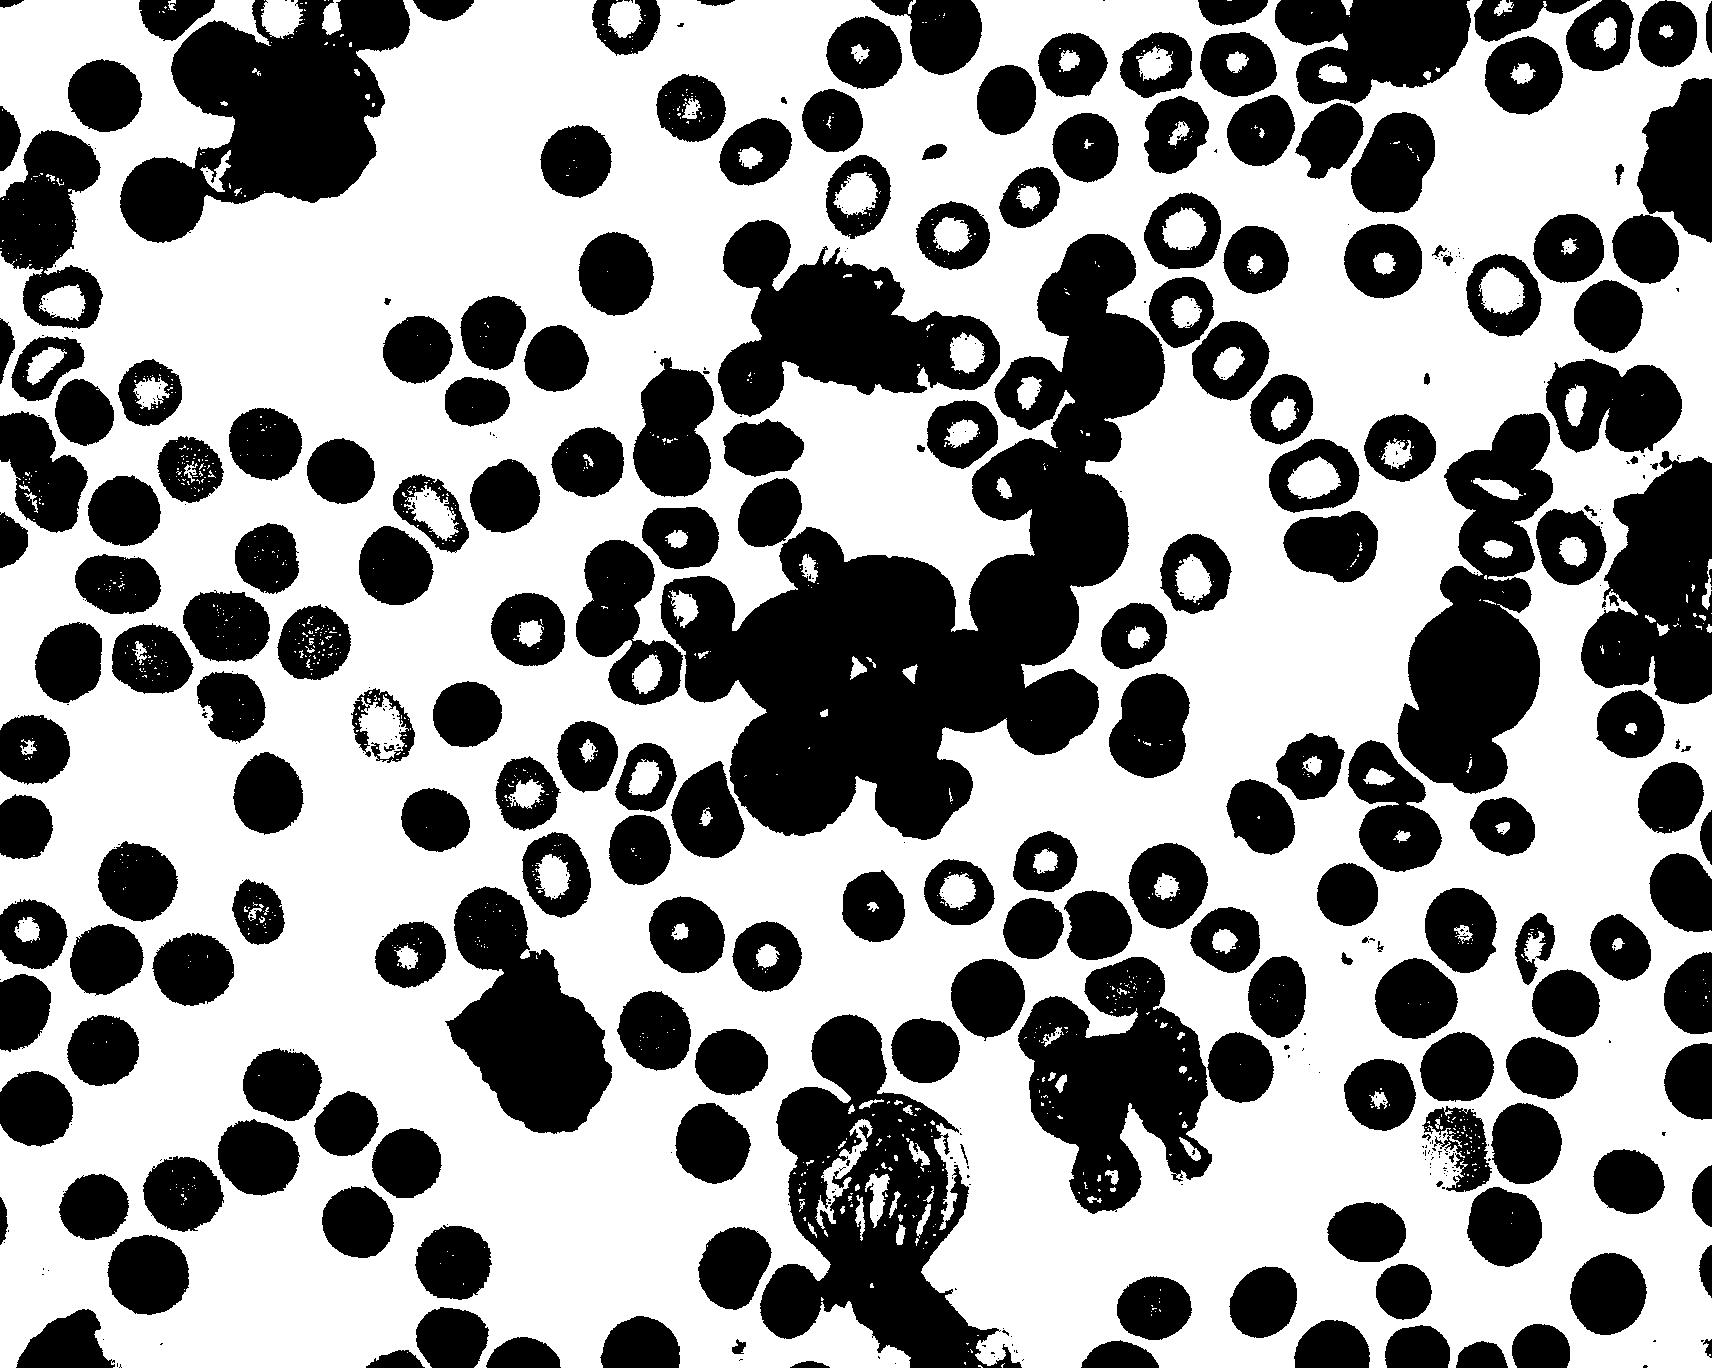
\includegraphics[width=0.3\textwidth]{images/fig_fuzzy2}
	\caption[Example of fuzzy thresholding.]{\label{fig:fuzzy}Example of fuzzy thresholding. From left to right: RGB original image; 2 class c-means fuzzy thresholded image (threshold value = 0.4347); 3 class c-means fuzzy thresholded image (threshold value = 0.7362).}
\end{figure}


\subsection{Local Thresholding} \label{LT} % DONE
Global thresholding algorithms may work properly in an area but produce unsatisfactory results in other areas when the background is not constant, and the contrast between objects varies unevenly. In this case, the use of local thresholding could be a better solution. The image is subdivided into rectangular overlapping sub-images, and the histogram of each of them is calculated. The sub-images must be big enough to include both the object and the background pixels. If the sub-image has a bimodal histogram, the minimum value between the two peaks is precisely the threshold. If the histogram is unimodal, the threshold value must be calculated by interpolating the thresholds of the adjacent sub-images, instead. In general, the local thresholding is computationally more expensive than the global one, although it is advantageous to segment objects from the background and to extract tiny and scattered variable regions. Fig. \ref{fig:localT} shows an example.

\begin{figure}[h]
	\centering
	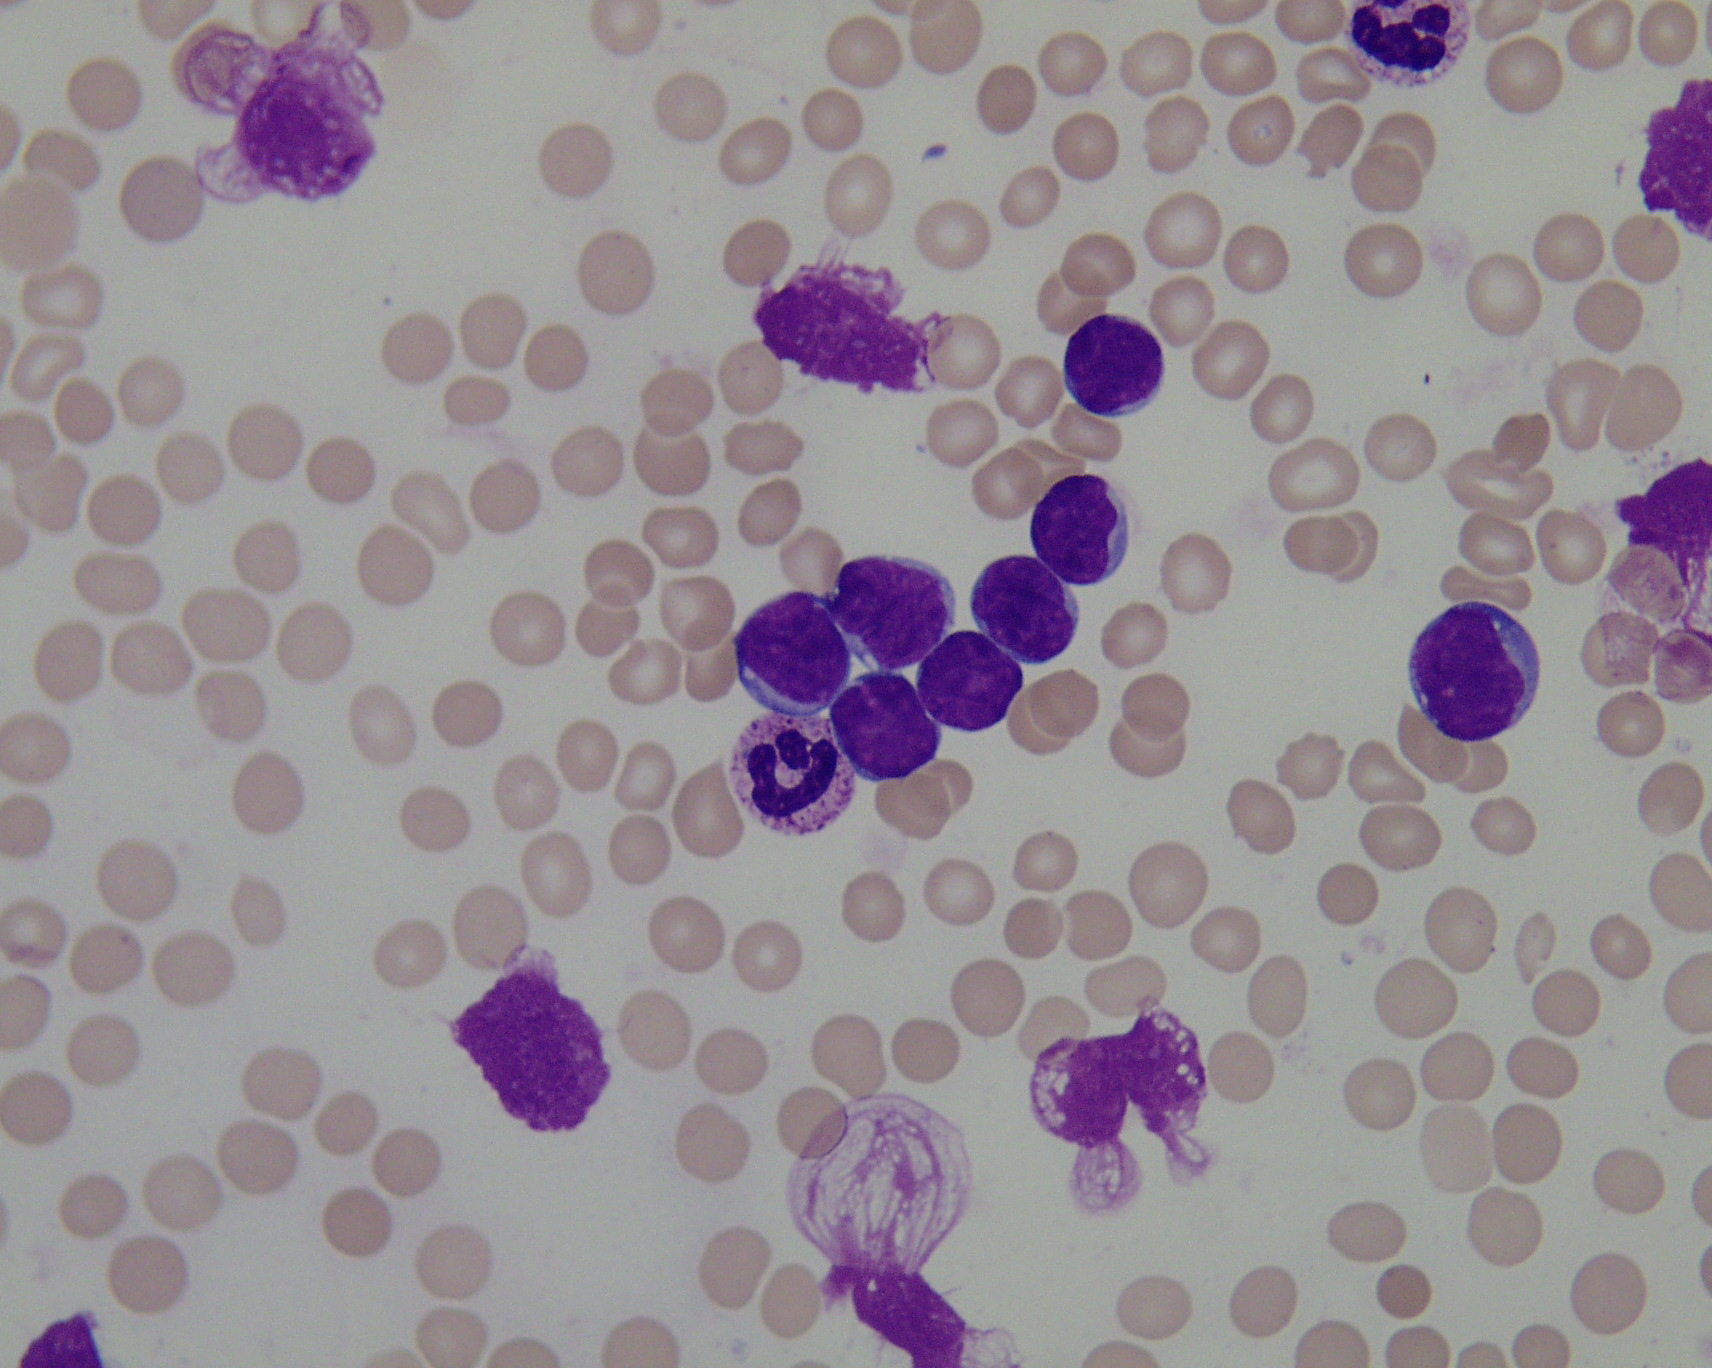
\includegraphics[width=0.45\textwidth]{images/figcs_rgb}
	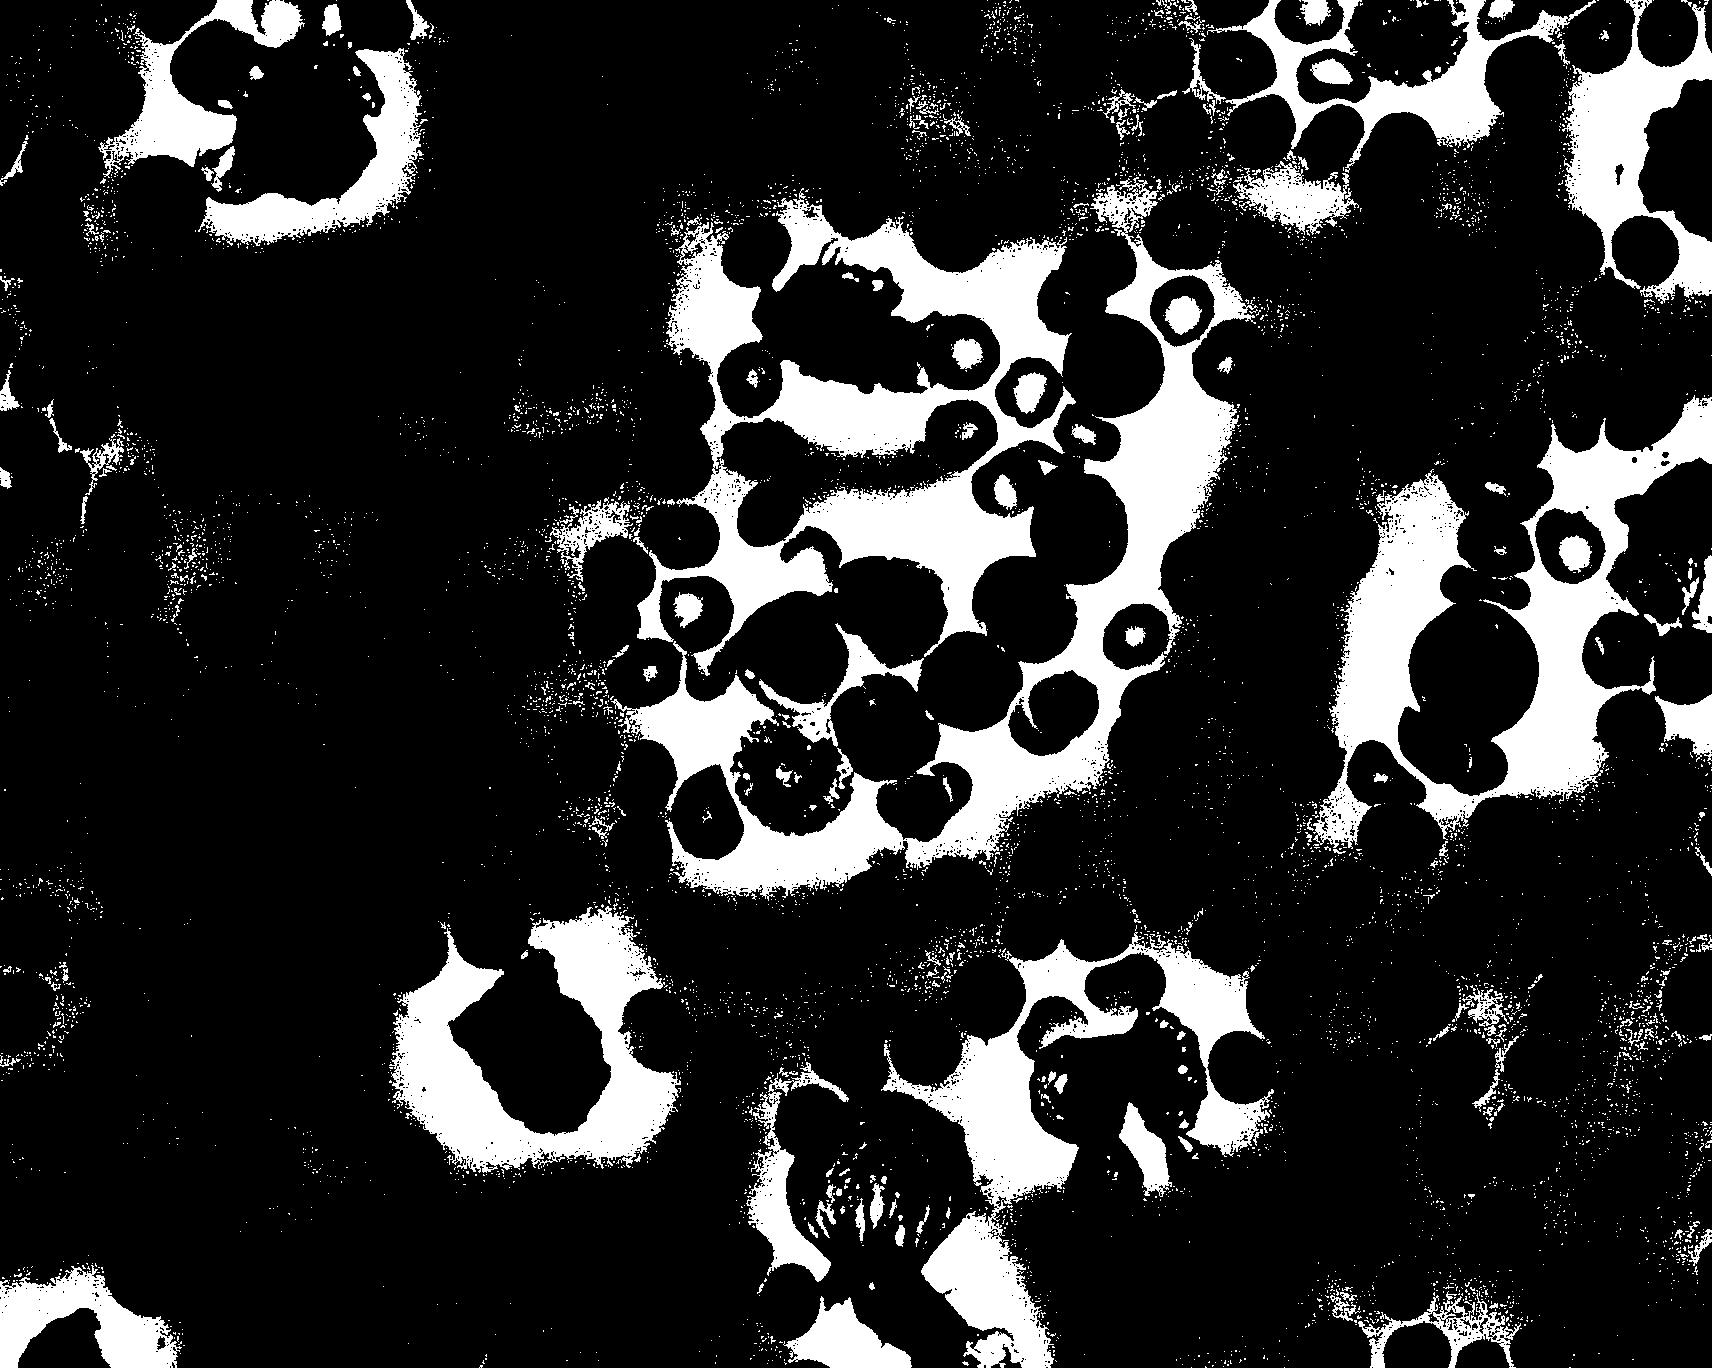
\includegraphics[width=0.45\textwidth]{images/fig_localT}
	\caption[Example of local thresholding.]{\label{fig:localT}Example of local thresholding. Left: RGB original image; local thresholded image with uniform sensitivity given to pixels belonging to background and everything else. WBCs zones are well distinguished from the other objects.}
\end{figure}

\section{Edge Based}
This segmentation technique is not based on the intensity value of the pixels, but on the fact that an object to be identified must have a closed edge that surrounds it. This assumption is not always true but often verified. The edges of objects are preliminarily identified by applying suitable operators of edge detection. As said previously, an edge is a set of connected pixels (4 or 8 connected) that lies on the border of two regions, therefore presenting sharp brightness changes. There is a little difference between edge and boundary since the edge is a local concept while the boundary is an extended concept. Therefore the boundary of an object is composed of a series of edges.
It is possible to carry out a threshold applied to the first derivative to detect only the edge. It is an operation that takes the name of non-maxima suppression, as it resets all the values in the first derivative which are not maximum. The chosen threshold value allows selecting more than one maximum points, as to have a contour wider but visible. Instead, if the threshold operation is applied to the second derivative, this operation takes the name of zero crossing and has the aim of seeking zero crossing points, necessary for the location of the edge points without distortion, avoiding the appearance of a double border. As previously mentioned, there are several implementations of filters on the first derivative, that can be applied directly to the search of the edges. In general, before the edge detection, a smoothing filter is applied to the image, to reduce both the noise and the edge thickness, so that the detection is more effective. The process works correctly if the signal is not noisy and if the edge is entirely localized in space and with small amplitude. An evolution of this approach is the Laplacian of Gaussian (\acs{LoG}) filter with zero crossing and the Canny filter with non-maxima suppression.
Examples are shown in Fig. \ref{fig:edge}.

\subsection{LoG Operator} % DONE
This edge detection approach, also known as Marr-Hildreth algorithm \cite{Marr}, is based on the second derivative of a function. The Laplacian operator is rarely used by itself for edge detection, as it is susceptible to noise, but it is used in conjunction with the Gaussian one, known precisely as Laplacian of Gaussian, LoG. The fundamental characteristics of LoG are the Gaussian smoothing filter, used to reduce noise and to enlarge the edge, the Laplacian in two dimensions, the zero crossings in the second derivative and, finally, the edge location estimated with sub-pixel using the linear interpolation. The Gaussian filter is preferred because it applies an action of smoothing both in space and in frequency. Furthermore, the derivative of the Gaussian filter is independent from the considered image and can be pre-calculated analytically by reducing complexity. Once the Laplacian filter is applied, it is needed to search points in the image in which there is a zero crossing, considering only those zeros for which there is a significant change in all possible directions around zero.

\subsection{Canny Operator}
Even the Canny algorithm \cite{Canny} uses a Gaussian filter for smoothing. Then the magnitude and direction of the gradient are calculated using different but finite approximations of partial derivatives. It applies the non-maxima suppression to the magnitude of the gradient, and finally, it uses the double threshold algorithm to find and link the edges. The use of the double threshold is necessary, considering that a single threshold would not lead to satisfactory results. For example, if the threshold is too low, it may detect too many false edges instead, if the threshold is too high some real edges may be lost. The use of two thresholds produces two different images and, of course, the image with the higher threshold will present a much smaller number of edges. Starting from this image, each edge is examined and compared with that one of the other images in search of edges that have been lost, and that can be linked to create a continuous boundary.

\begin{figure}[h]
	\centering
	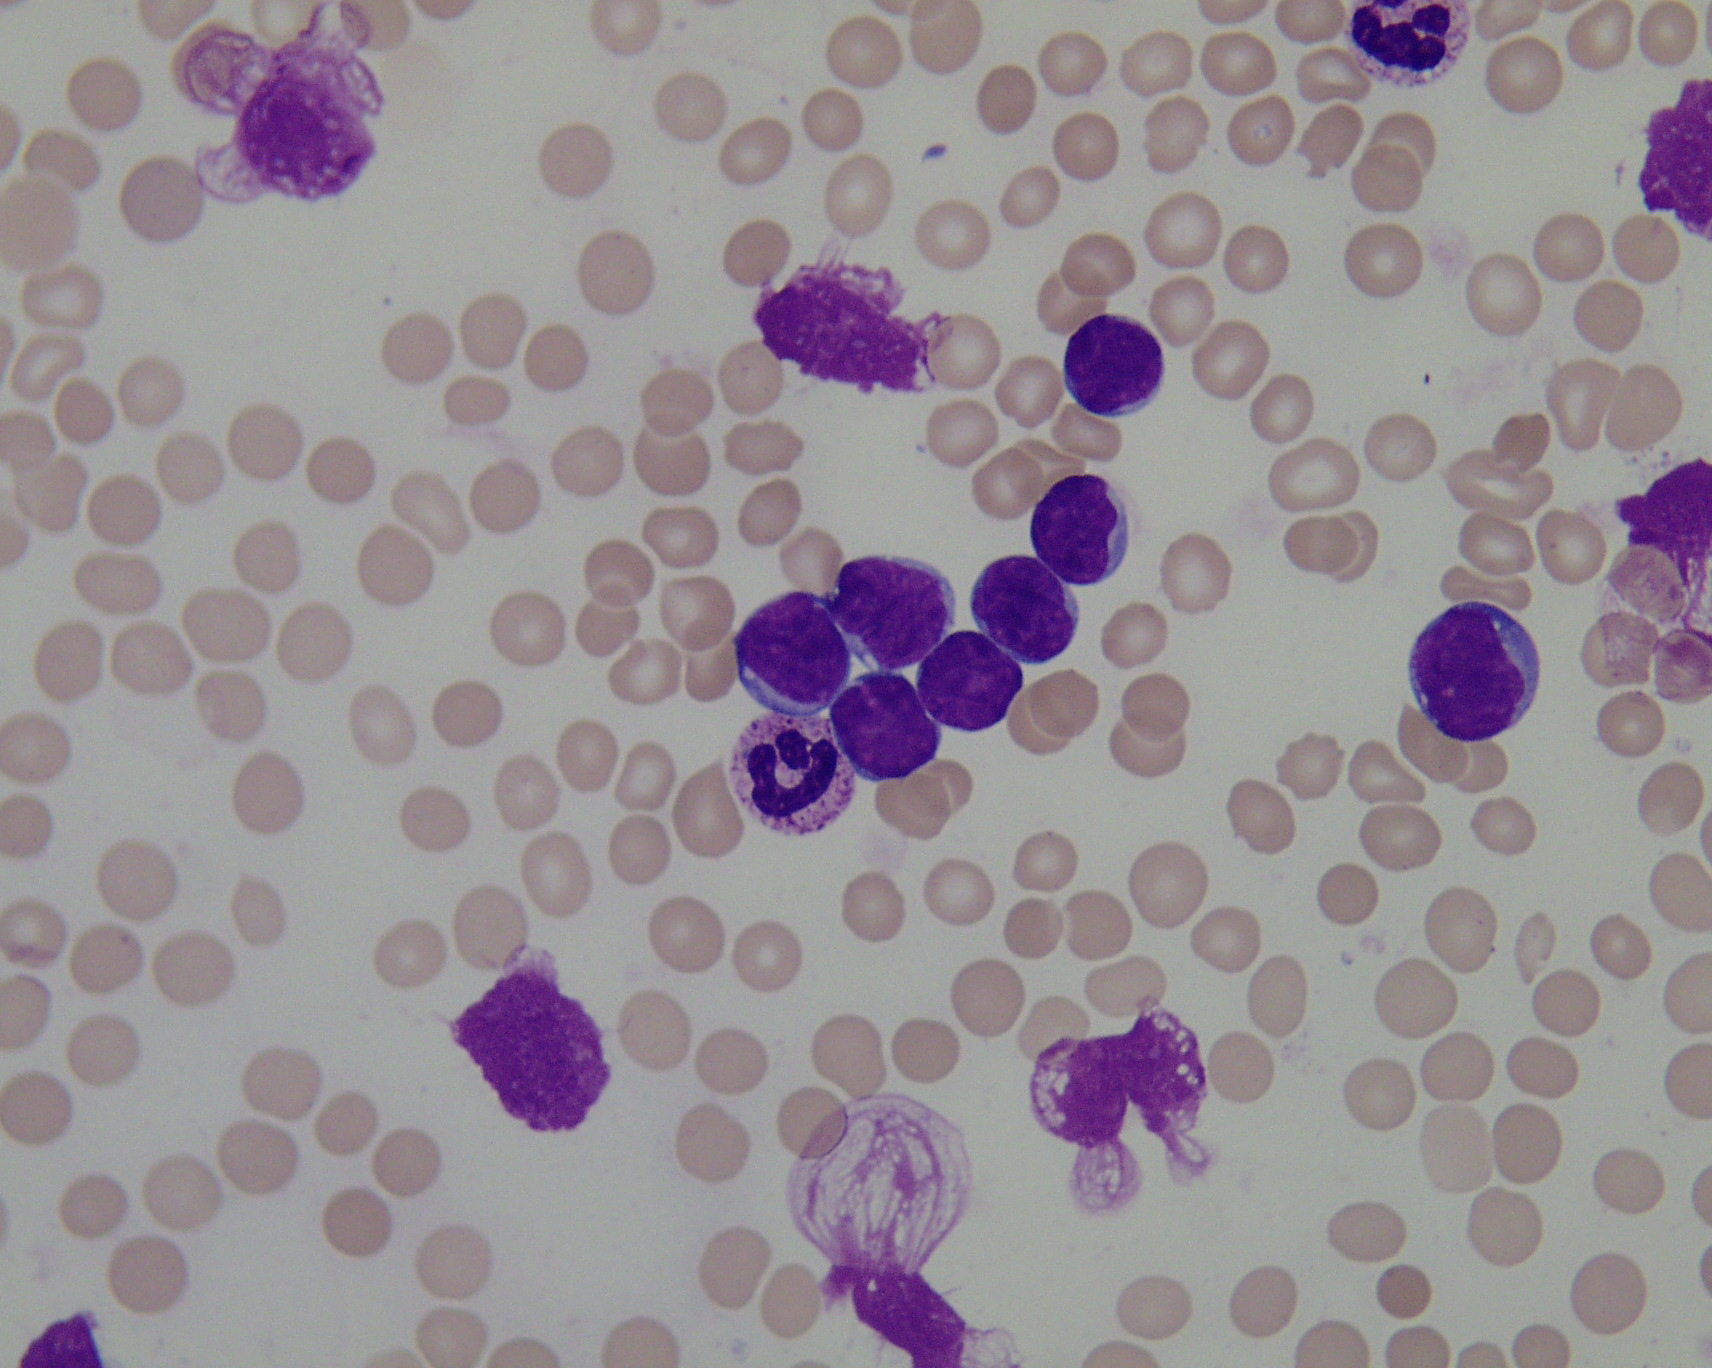
\includegraphics[width=0.3\textwidth]{images/figcs_rgb}
	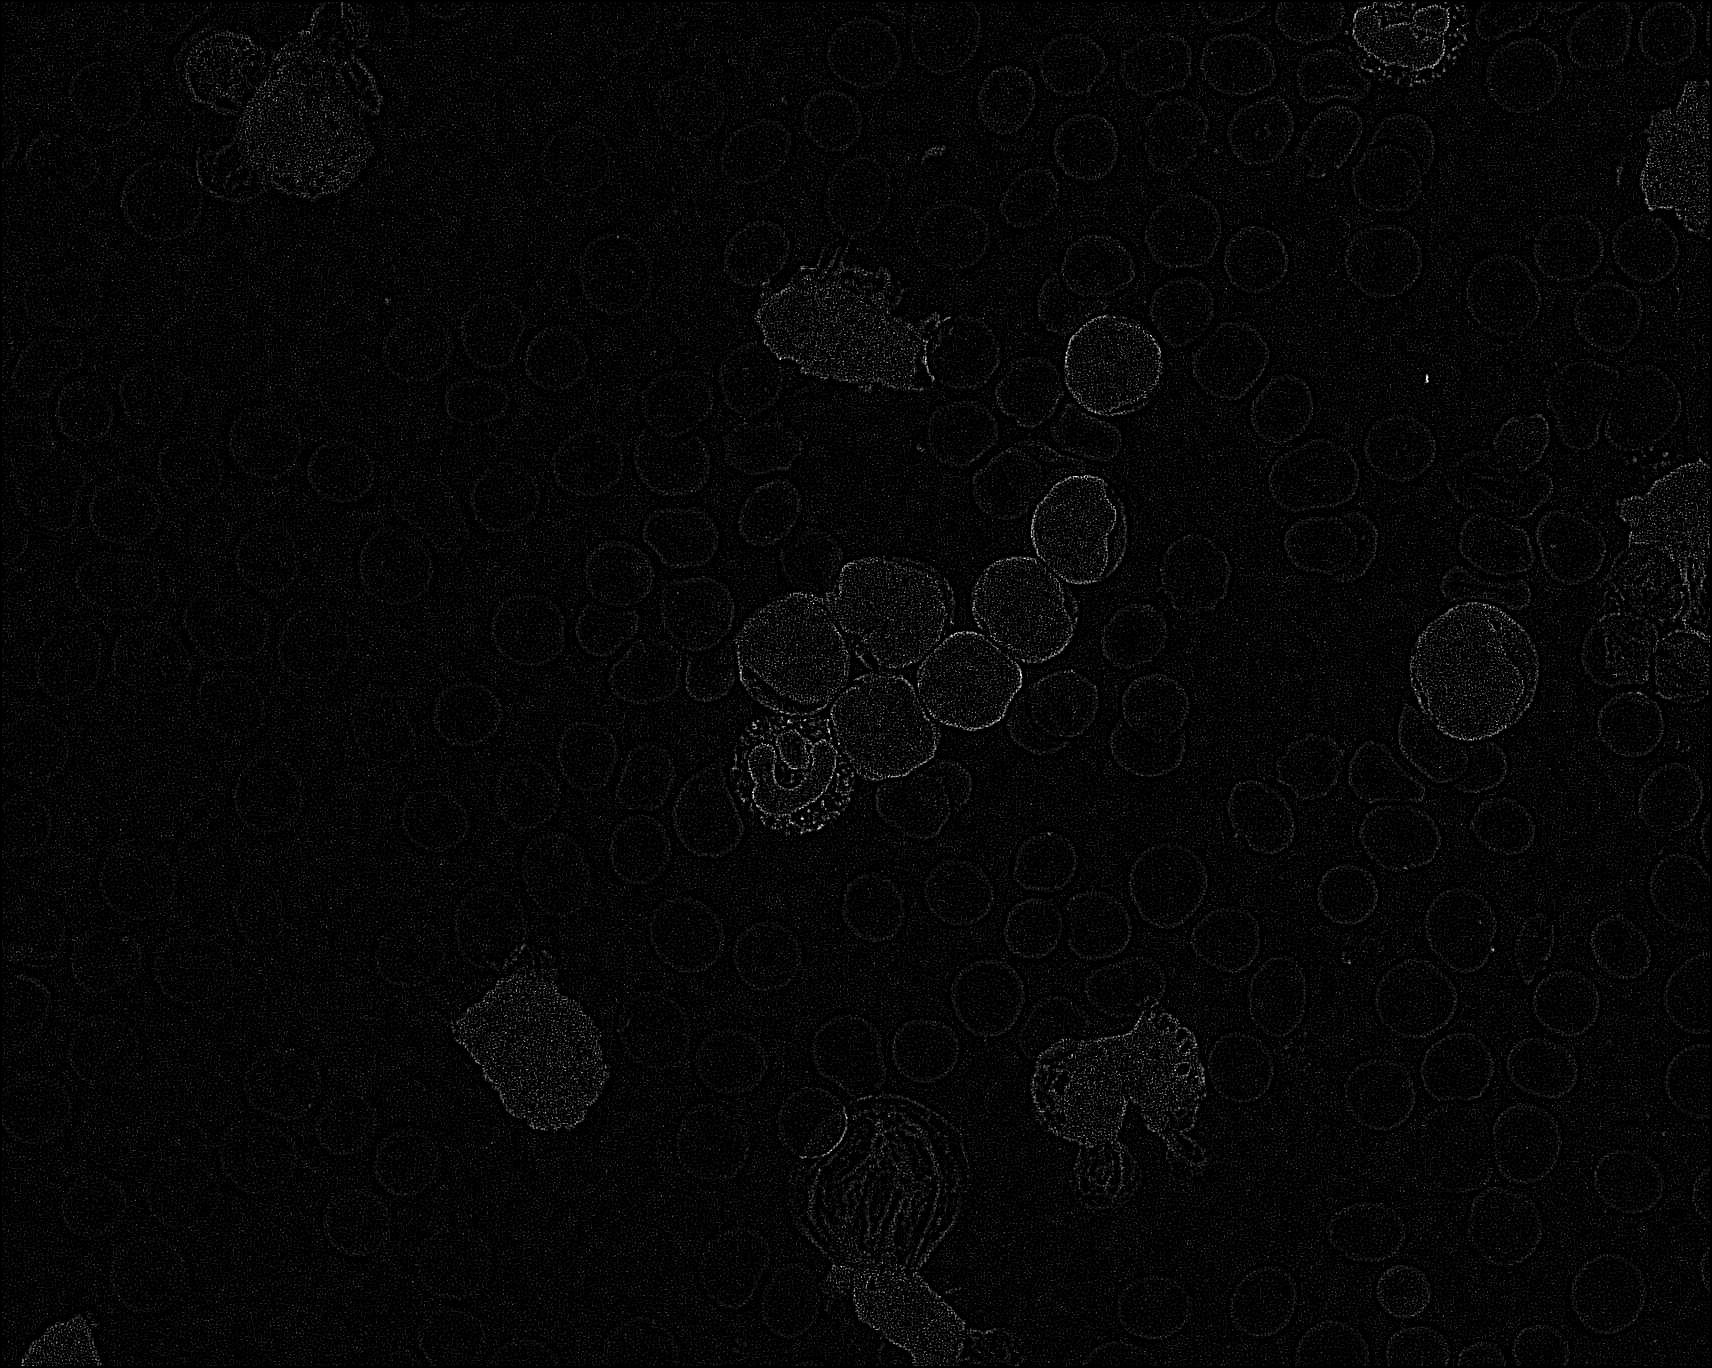
\includegraphics[width=0.3\textwidth]{images/fig_OpLog}
	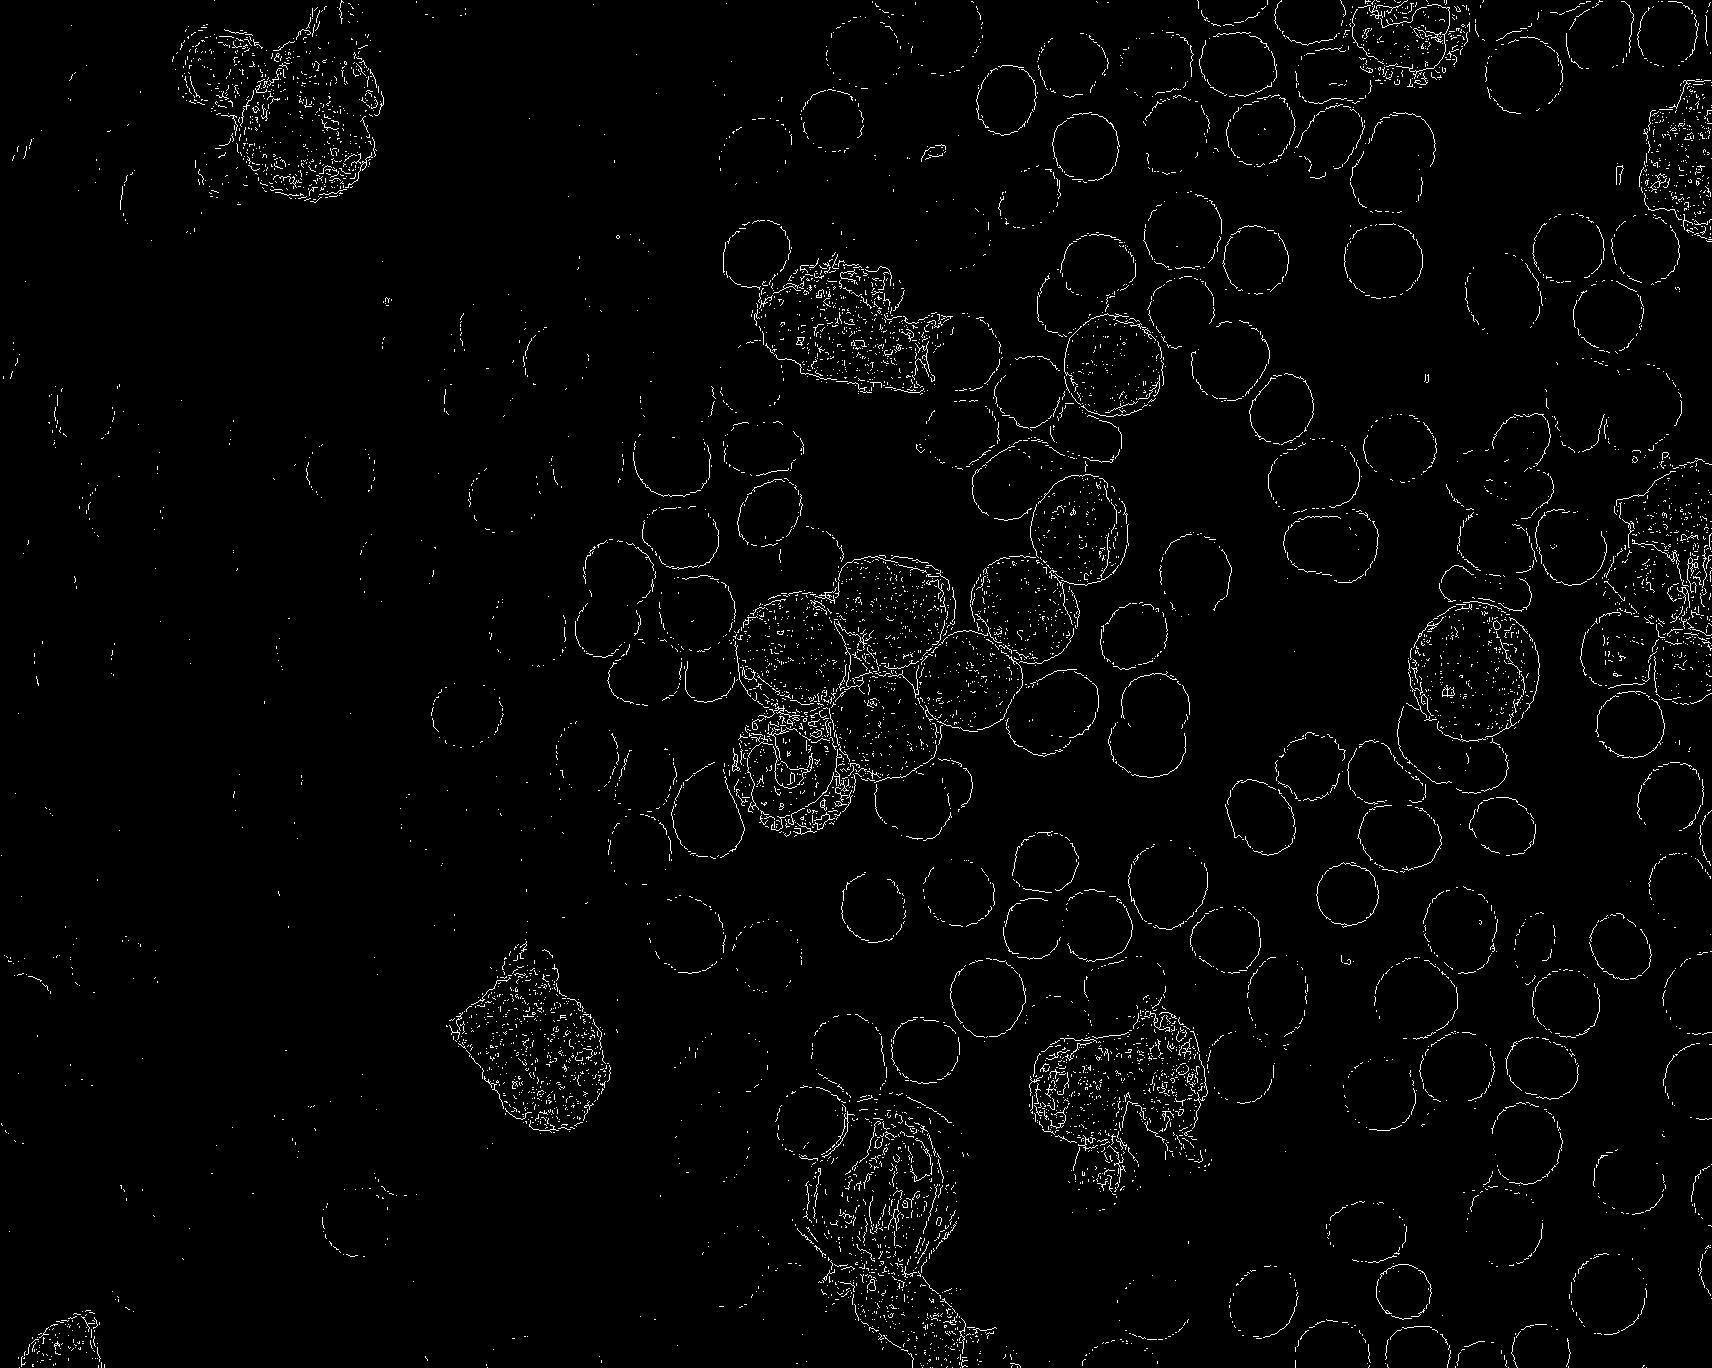
\includegraphics[width=0.3\textwidth]{images/fig_OpCanny}
	\caption[Edge based segmentation.]{\label{fig:edge}Example of edge based segmentation. Left: RGB original image; binary mask obtained with LoG operator; binary mask obtained with Canny operator.}
\end{figure}

\subsection{Deformable Models} 
In medical image analysis, in many cases, the boundaries between the tissue structures and cell components are not clearly defined. The use of edge detection on these images produces poor results, in particular, due to the presence of small structures or particles this approach produces a huge number of false edges. Moreover, in general, the edge approaches based on filters do not yield to a closed contour. As a result, these techniques either fail or require some post-processing step to remove invalid object boundaries in the segmentation results or to close the extracted contour. To address these difficulties, deformable models or snakes \cite{Kass} have been extensively studied and widely used in medical image segmentation, with promising results, as shown in Fig. \ref{fig:snakes}. Deformable models are curves or surfaces defined to match a contour as an energy minimization problem, where the optimal solution constitutes an equilibrium of internal and external energy. The deformable model can move under the influence of internal forces, which are defined within the curve or surface itself to keep the model smooth during deformation, while external forces, which are computed from the image data, are defined to move the model toward an object boundary or other desired features within an image. By constraining extracted boundaries to be smooth and incorporating other prior information about the object shape, deformable models offer robustness to both image noise and boundary gaps.

\begin{figure}[h]
	\centering
	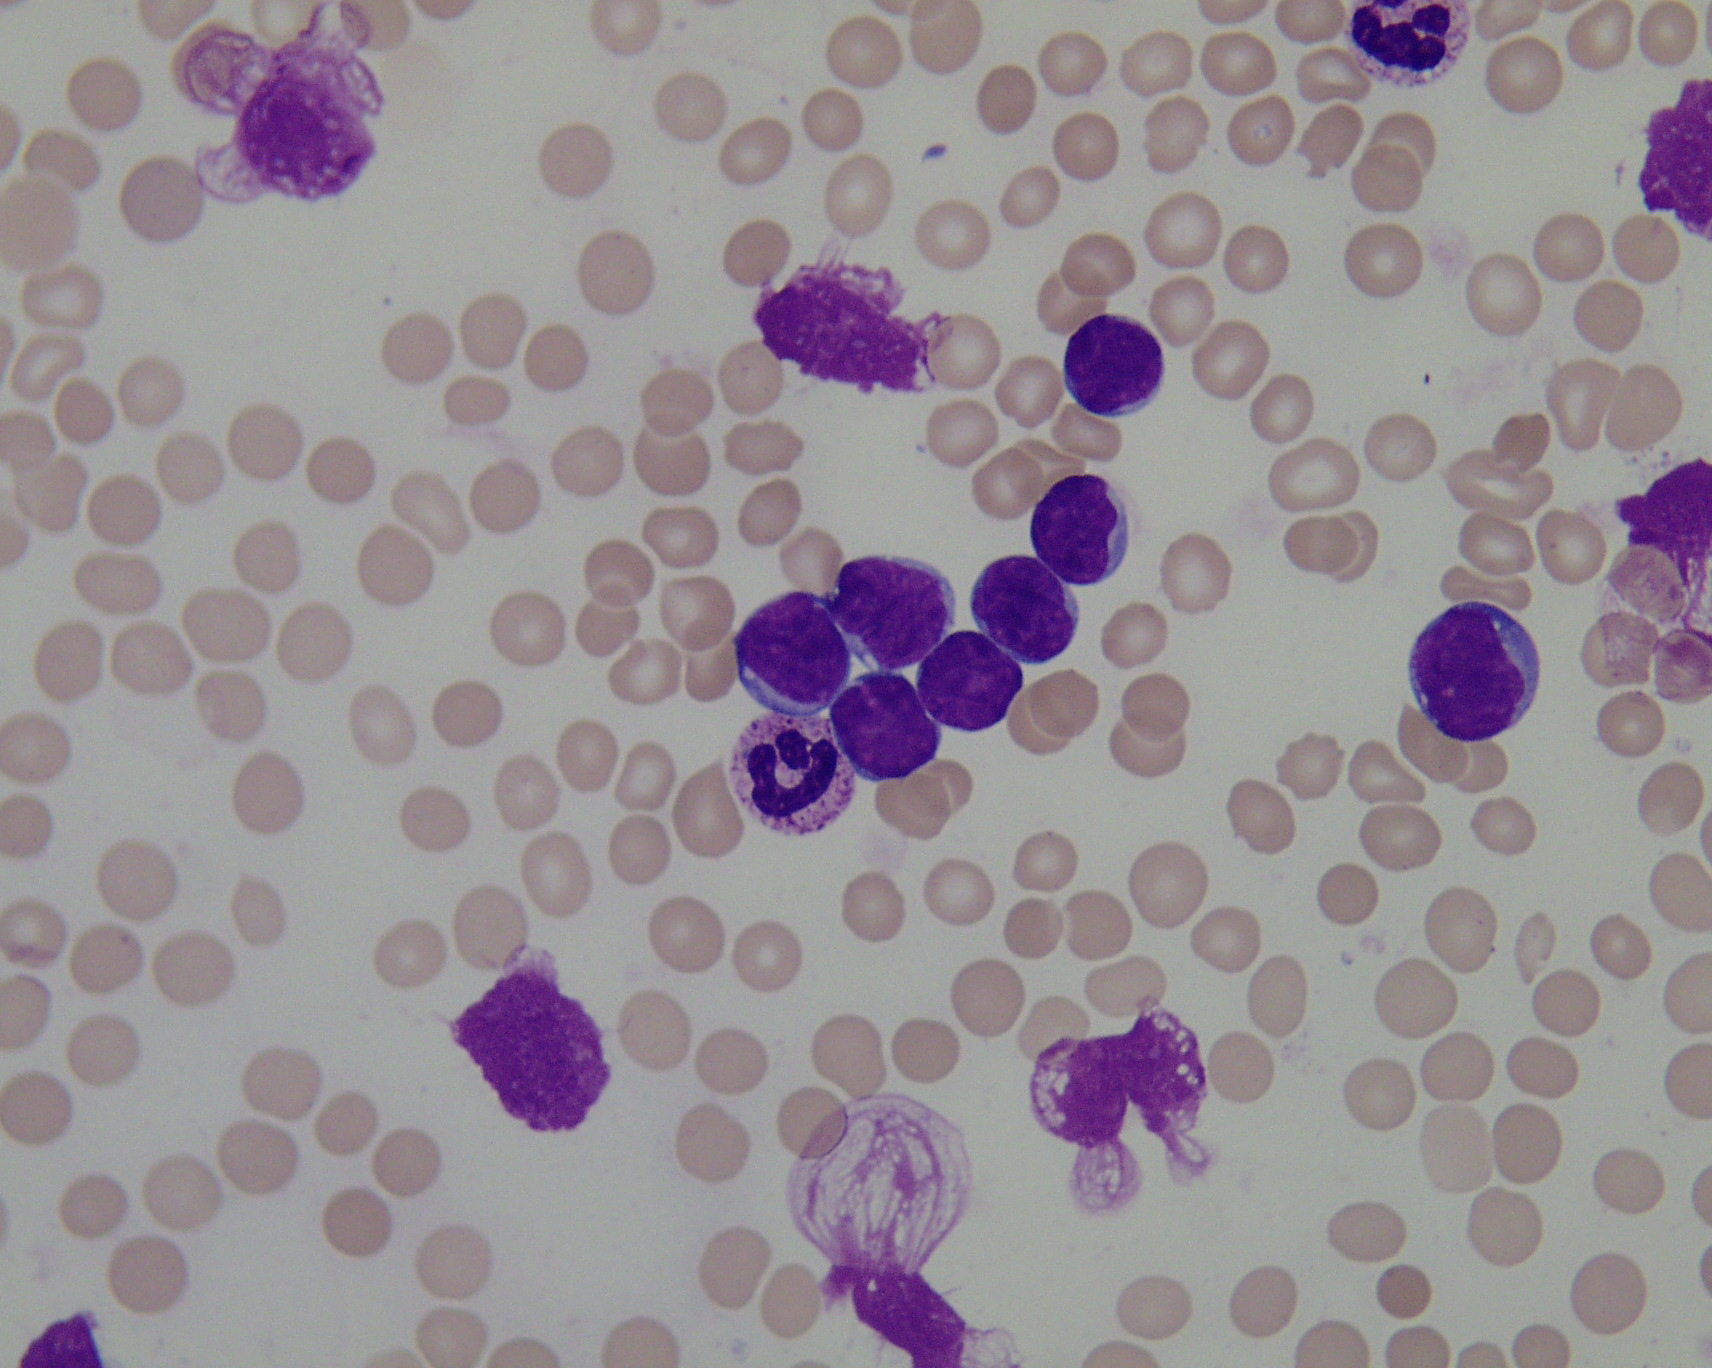
\includegraphics[width=0.3\textwidth]{images/figcs_rgb}
	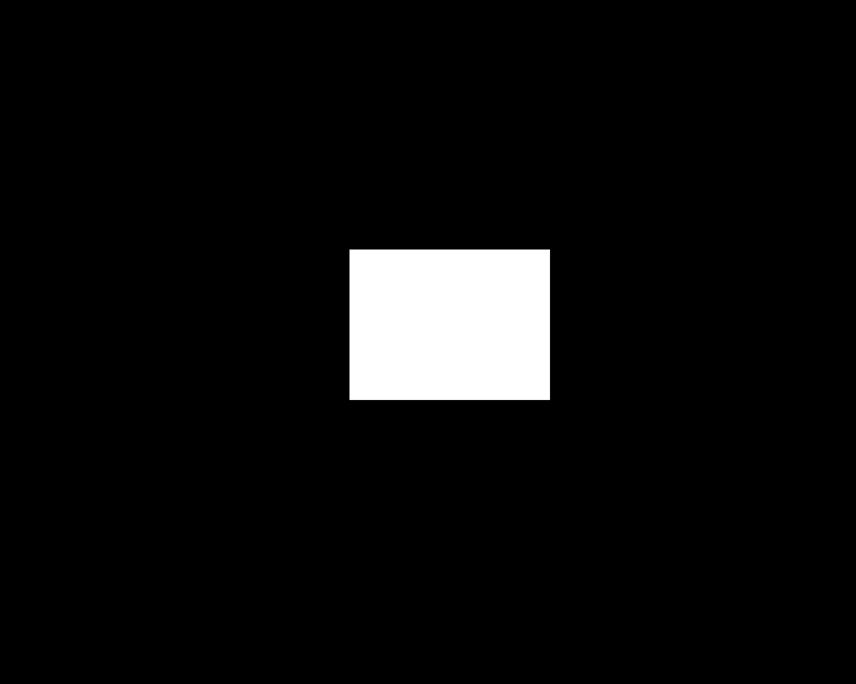
\includegraphics[width=0.3\textwidth]{images/fig_snakes1}
	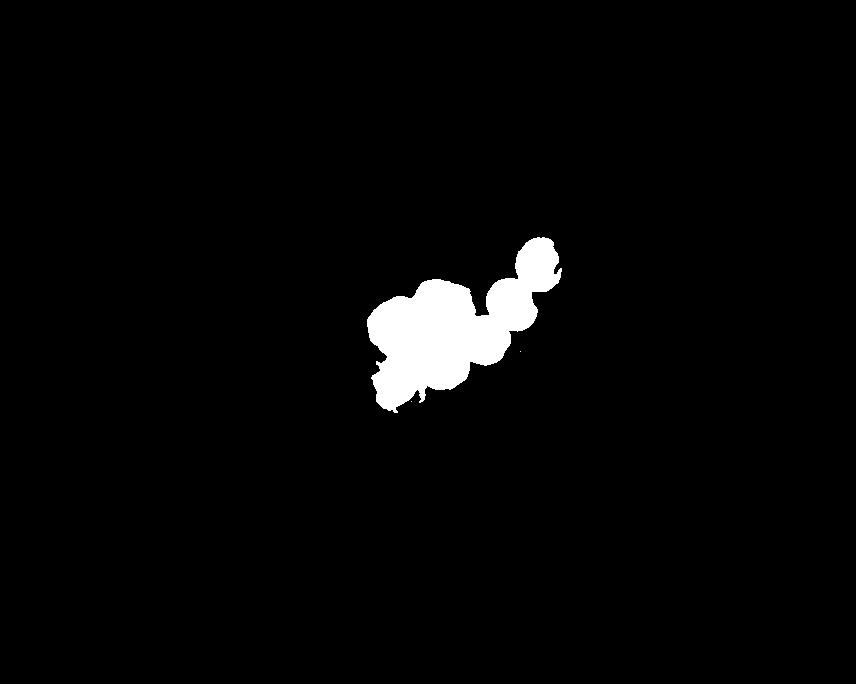
\includegraphics[width=0.3\textwidth]{images/fig_snakes2}
	\caption[Example of Active Contour.]{\label{fig:snakes}Example of deformable model segmentation, by using Active Contour strategy. From left to right: RGB original image; seed region indicates the region to analyse; segmentation result after 250 iterations of Active Contour.}
\end{figure}

\section{Region Based} 
These segmentation techniques introduce more information than previous concerning the connectivity of the pixels forming the entire object, avoiding in this way that individual points of the same region, having the right color or the right contrast, are classified as separate objects. Unlike the pixel and edge-based segmentation methods, region-based approaches aim to identify objects and regions, working directly on the space occupied by the pixels instead of identifying objects from their properties, such as brightness or edges. Considering $R$ as the entire spatial region occupied by the image, the segmentation process can be seen as the partitioning of $R$ into $n$ sub-regions $R1, R2, ..., Rn$, with the constraint that, the union of all regions returns $R$ and the intersection between any set of regions is equal to $0$. The pixels belonging to a region must be connected (8 or 4 connected), and a similarity criterion must relate them. The most common techniques of segmentation region based are divided into region growing and split and merge techniques.

\subsection{Region Growing} 
The region growing is a procedure that allows selecting regions connected and homogeneous of an image, whose selection is effected from a single pixel and is based on a similarity or growth criterion which imposes a maximum difference, a priori defined, between the value of the initial pixel and the pixel values of the region. The basic approach involves the selection of a set of starting pixels, called seed points, and from these seeds add the pixels of their neighborhood that have specific properties of similarity with the seeds, such a specific intensity range or color. The selection of the set of starting pixels is based on the nature of the problem, instead the selection criteria of similarity depends both on the problem and the type of the input image, since it must be ensured independence between the result of the segmentation and the scan direction of the image or the selected seed points. 

Algorithms of region growing have been widely used for the analysis of peripheral blood images, in particular for segmentation of cells in which the nucleus is easily identifiable and thus can be used as a seed, as shown in Fig. \ref{fig:regionGrowing}. 

\begin{figure}[h]
	\centering
	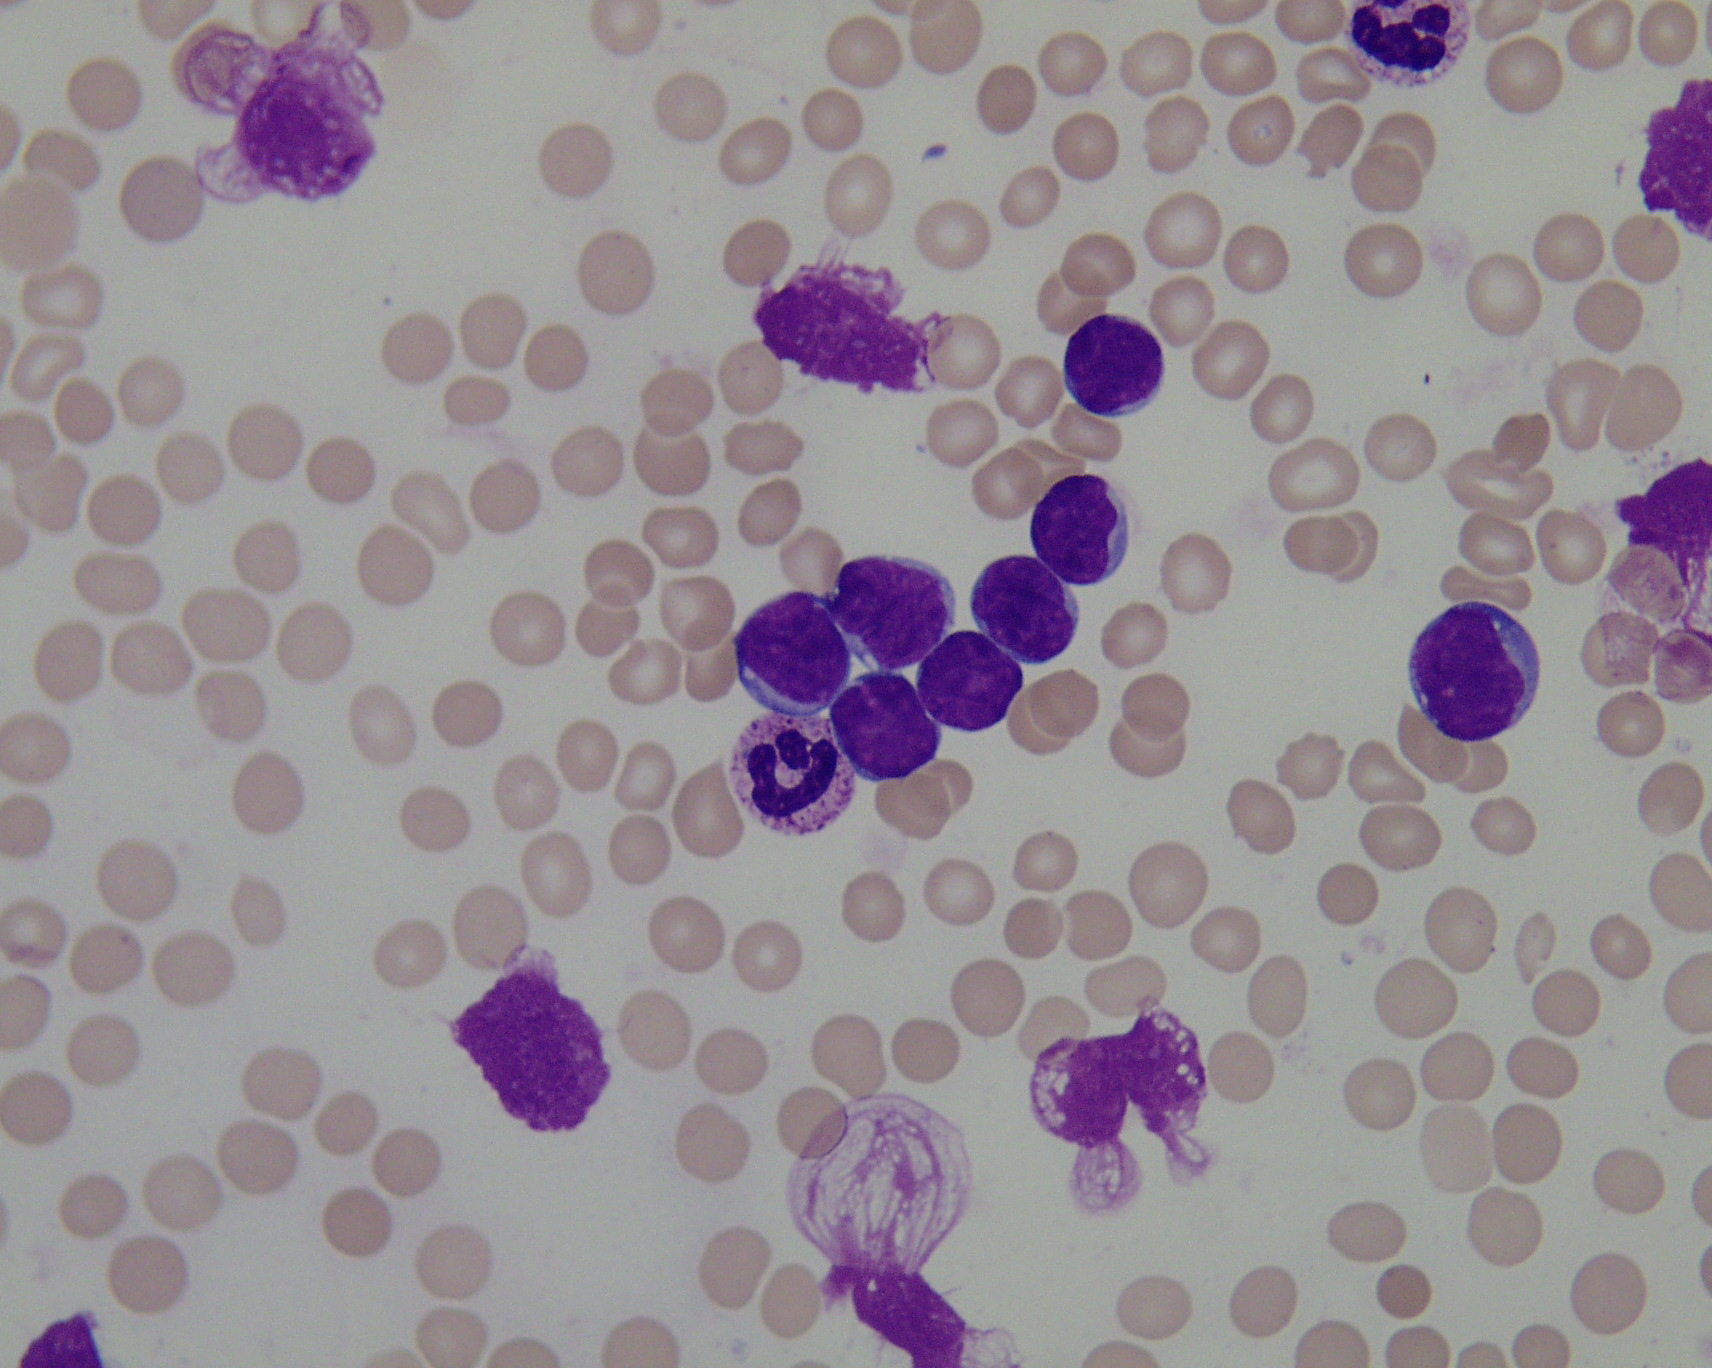
\includegraphics[width=0.3\textwidth]{images/figcs_rgb}
	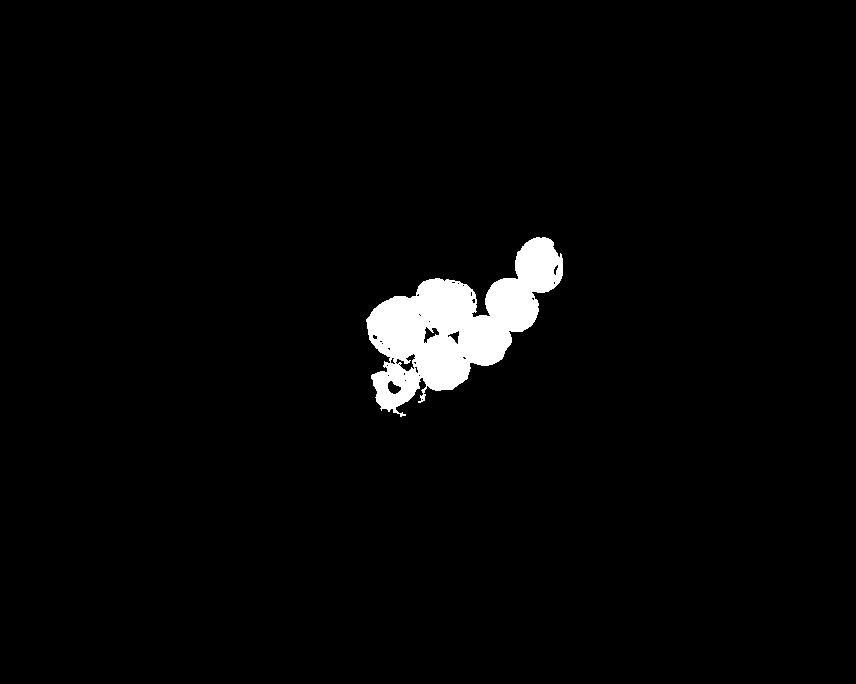
\includegraphics[width=0.3\textwidth]{images/fig_regionGrowing}
	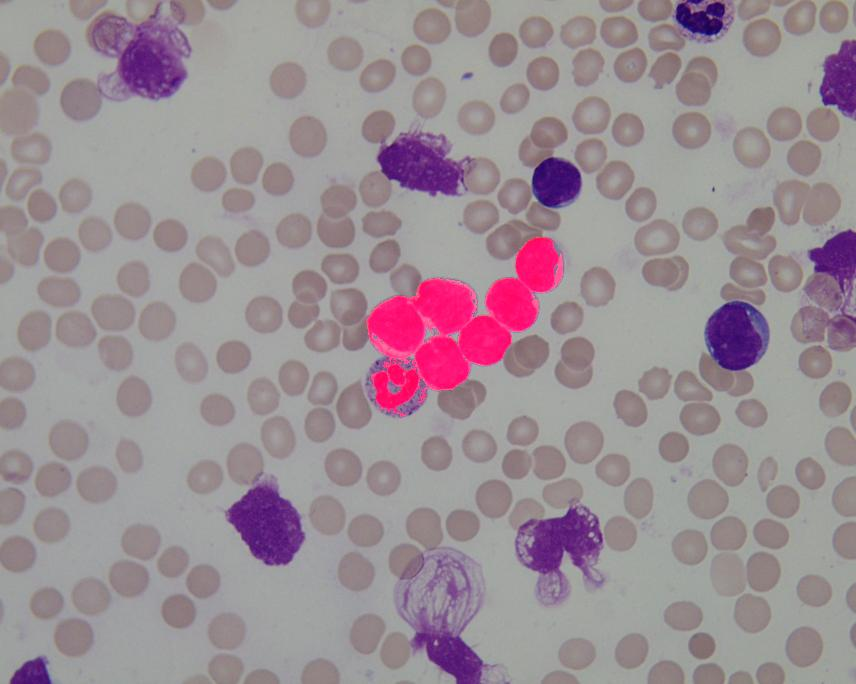
\includegraphics[width=0.3\textwidth]{images/fig_regionGrowing2}
	\caption[Example of region growing.]{\label{fig:regionGrowing}Example of region growing application. From left to right: RGB original image; segmentation result after region growing application starting from a WBC nuclei seed point in the centre of image; superimposition of segmentation result over original image indicating the obtained region.}
\end{figure}

\subsection{Split and Merge} 
Segmentation can also be performed by recursively splitting (partitioning) an image until uniform regions are obtained. Then, merging (aggregation) can be performed on adjacent regions that may be compatible on the basis of a similarity criterion. In the simplest way, an image can be partitioned recursively repeating a division into four quadrants, until uniform smaller regions (even composed of a few pixels) have been obtained, according to the defined similarity criterion. Such division into quadrants is represented by a tree called quad-tree, in which the root node contains the information of the whole image and each of the four children nodes contains the information about a quadrant. If a quadrant is sufficiently uniform, it will not be further partitioned. Splitting step inevitably partitions also homogeneous regions and makes necessary a subsequent phase to merge the adjacent and homogeneous regions of the image into a region that meets the defined criterion of similarity, as shown in Fig. \ref{fig:splitMerge}.

\begin{figure}[h]
	\centering
	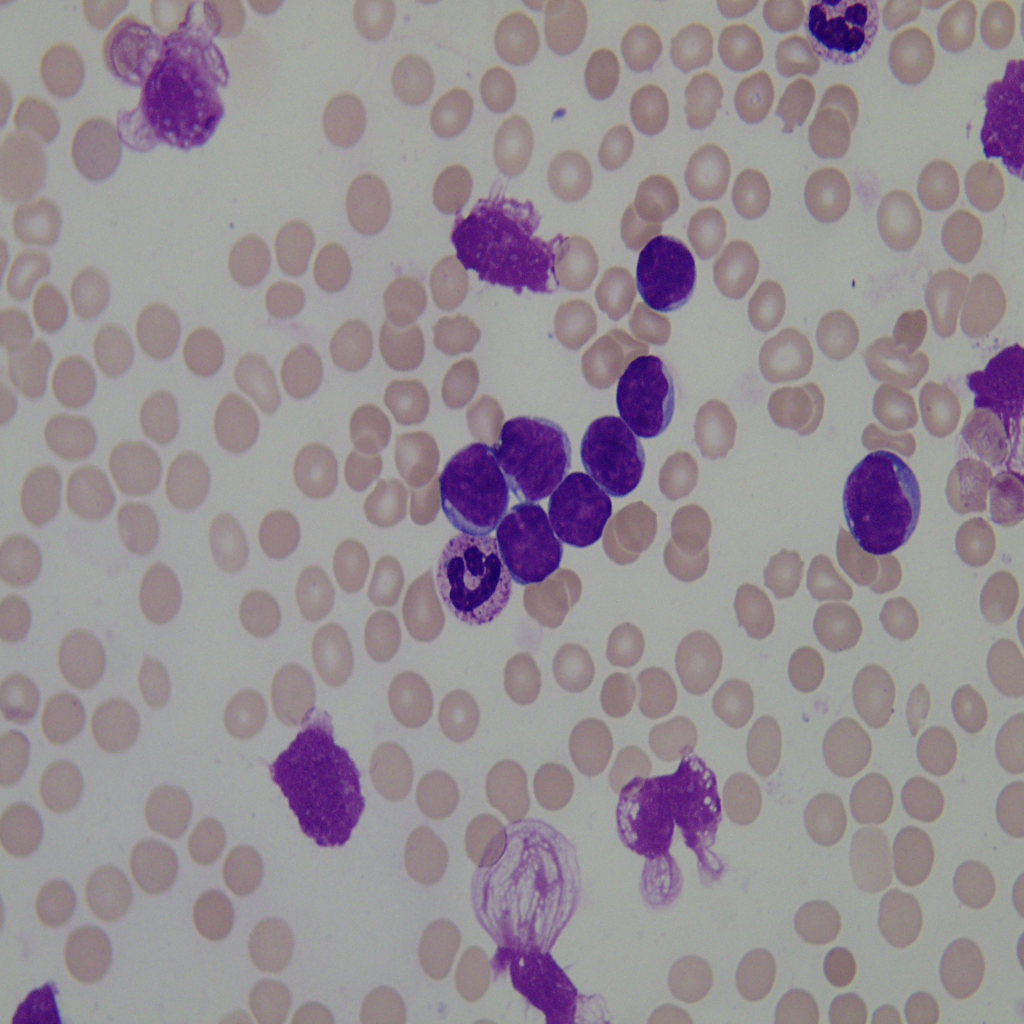
\includegraphics[width=0.3\textwidth]{images/fig_rgbSplitMerge0}
	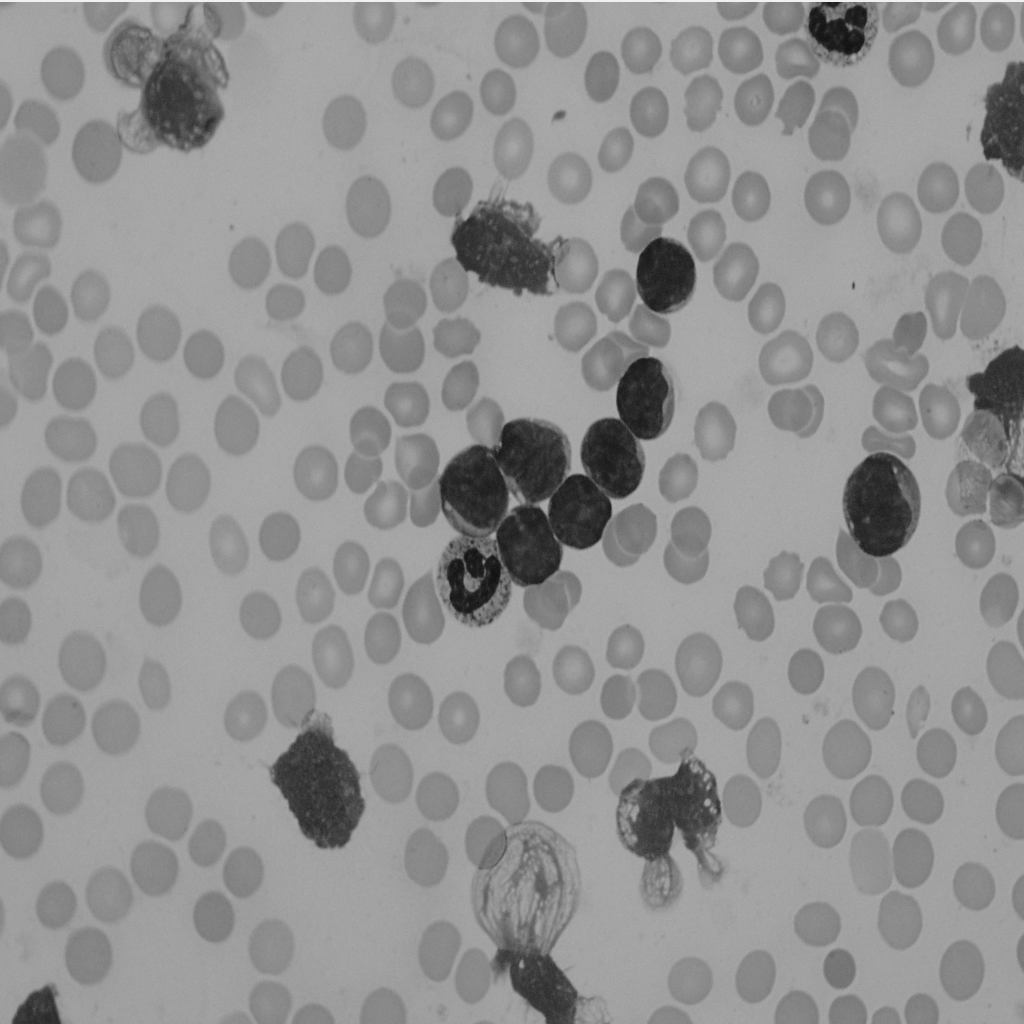
\includegraphics[width=0.3\textwidth]{images/fig_rgbSplitMerge1}
	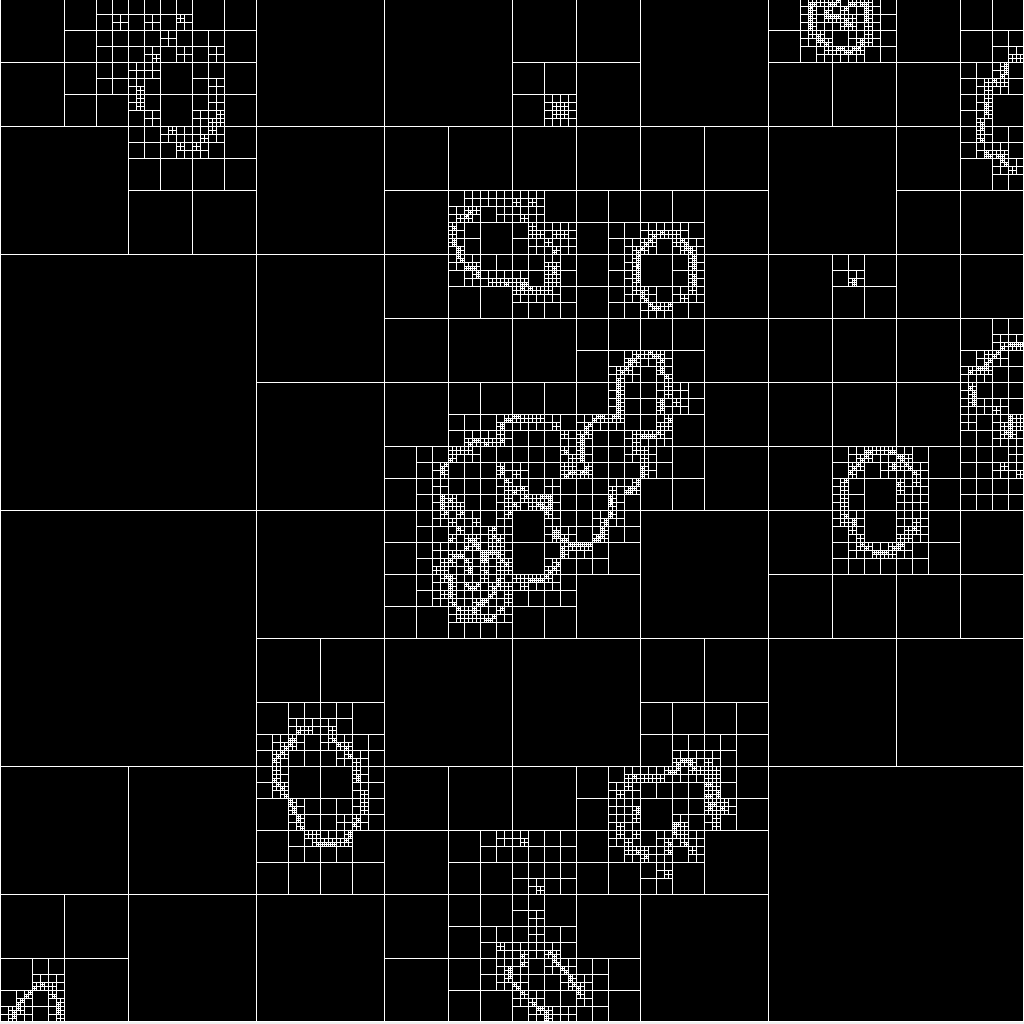
\includegraphics[width=0.3\textwidth]{images/fig_splitMerge}
	\caption[Example of split and merge.]{\label{fig:splitMerge}Example of split and merge application. From left to right: RGB original image; gray level converted image; split and merge segmentation results by using quadrants from $512 \times 512$ down to $1 \times 1$.}
\end{figure}

\subsection{Watershed} \label{watershed} % DONE
The watershed segmentation \cite{Meyer} is a mixed approach based on the pixel aggregation (flooding) with the use of the image gradient as a barrier for flooding. In this approach, the gradient image can be considered as a topographical 3D image, in which it is possible to identify points that come from a regional minimum, points that surely fall in a local minimum called basin and points of local maximum called watershed lines. The flooding applied to this image leads to a state where only the watershed lines are visible, that correspond to the objects contours in the image. A direct application of the watershed algorithm induces an over-segmentation due to the presence of too many basins which can never merge, or the presence of noise and other irregularities of the gradient. To avoid this problem in digital microscopy images analysis, the watershed is often used with different strategies that include the use of markers. These markers can be extracted directly from the original images intensity value and subsequently combined with the gradient to obtain a stronger result.

\section{Post-Processing} \label{postp}
After segmentation, an image can be represented as a map of binary objects, background, and foreground. In some cases, the initial segmentation is not satisfactory, as it can present holes or artifacts. Some improvements to the segmentation results can be made directly on the binary image using a series of operations based on an a priori knowledge. The morphological operators are commonly used for this purpose, to reduce the number of artifacts, to fill the holes present in some regions, to remove some objects not completely enclosed in the image or others that are not interesting for the analysis. Mathematical morphology is based on the set theory for binary images \cite{Serra, Serra2} and on lattice theory for grey level images. It provides some approaches to image processing that are useful to extract image components and for the representation and description of the object's shape. The sets, in this case, represent the objects contained in the image. The operations of mathematical morphology are based on the use of structuring elements, that are small sets of sub-images used to investigate and study the properties of interest in the input image. They can have any shape defined according to the problem to be treated and are represented as binary matrices.

\subsection{Mathematical morphology} % DONE
Mathematical morphology (MM) can be defined as a theory for the analysis of spatial structures. It is called morphology because it aims at analyzing the shape and form of objects. It is mathematical in the sense that the analysis is based on set theory, integral geometry, and lattice algebra. MM is not only a theory but also a very powerful image analysis technique \cite{Soille2004}.
It was introduced by Matheron in 1964 as a technique for analyzing the geometric structure of metallic and geologic samples. It refers to a branch of nonlinear image processing and analysis that concentrates on the geometric structure within an image.
The morphological filters, which can be constructed on the basis of the underlying morphological operations, are more suitable for shape analysis than the standard linear filters since the latter sometimes distort the underlying geometric form of the image. Some of the salient points regarding the morphological approach are as follows \cite{Giardina1988}:
\begin{itemize}
	\item Morphological operations provide for the systematic alteration of the geometric content of an image while maintaining the stability of the important geometric characteristics.
	\item There exists a well-developed morphological algebra that can be employed for representation and optimization.
	\item It is possible to express digital algorithms concerning a tiny class of primitive morphological~operations.
	\item There exist rigorous representation theorems by means of which one can obtain the expression of morphological filters in terms of the primitive morphological operations.
\end{itemize}

MM was initially developed for binary images and later generalized to greyscale images \cite{Soille2004, Serra1984}, considered as a sampled function of $\mathbb{R}^{2}$ in $\mathbb{R}$, or in general of any function of $\mathbb{R}^{n}$ in $\mathbb{R}$.
More recently, several researchers have extended morphological operators to color (or in general multispectral) images, considered as sampled functions of $\mathbb{R}^{n}$ in $\mathbb{R}^{m}$, with $m$ being equal to three in the case of the usual color images or the number of bands otherwise \cite{Benavent2012}.  Moreover, several approaches for fuzzifying MM have been proposed, extending the ordinary morphological operations by using fuzzy sets \cite{Kerre2000}.

Dilation and erosion are the basic morphological processing operations. They are defined in terms of more elementary set operations but are employed as the essential elements of many algorithms. Both~dilation and erosion are produced by the interaction of a set called structuring element (SE) with a set of pixels of interest in the image. The structuring element has both a shape and an origin. From these two basic operators, others have been derived (opening, closing, hit-or-miss). They can be applied to extract image components useful in the representation and descriptions of region shapes, such as area granulometry, boundaries, skeleton, or convex hull. Besides, morphological operators can be used for image preprocessing and postprocessing, such as morphological filtering, thinning, and~especially for segmentation.

Given an image or set $A$ and a structuring element $B$, the operations are realized by sliding $B$ over $A$ so that the origin of $B$ visit all elements of $A$. The \textit{erosion} operation creates a new set by considering all the location of $B$ for which $B$ is entirely contained in $A$. The result is that the contour of the set $A$ has been eroded. Such a property for which $B$ must be fully contained in $A$ is equivalent to the property for which $B$ must not share any elements with the complement of $A$. The erosion and dilation are dual operations; thus it is possible to obtain the dilation of $A$ through the use of a structuring element $B$ eroding the complement of $A$. More immediately, the \textit{dilation} operation creates a new set by considering all the location of $B$ for which at most one element of $B$ is contained in $A$. The result is that the contour of the set $A$ has been dilated. A simple operation that arises from the erosion is the \textit{boundary extraction}. The contour of a set $A$ can be obtained from the difference between the original set $A$ and the erosion of $A$ with an appropriate structuring element $B$.

Also, the opening and closing arise from the composition of erosion and dilation. The \textit{opening} of an image or set $A$ with a structuring element $B$ is defined as the erosion of $A$ with $B$ followed by a dilation of the result. This is useful to flatten the contours of an object, breaking the thin lines and removing the sharp contour. The \textit{closing} of an image or set $A$ with structuring element $B$ is defined as the dilation of $A$ with $B$ followed by the erosion of the result. Even the closing flattens the contours, but differently, in fact, it eliminates small holes and fills the gap in the contours. To fill bigger holes, instead, the operation of \textit{hole filling}, that consists of a more laborious process, is used. Assuming to have a set $A$ with a hole inside, the process starts taking the complement of $A$, that is composed of the background pixels and therefore also the hole pixels. Then, iteratively, a set containing only a pixel for each hole is dilated using an appropriate structuring element and making every time the intersection with the complement of $A$, so as to exclude pixels outside the contour of $A$.
Similarly, an iterative procedure of dilatation is used for the \textit{extraction of connected components}. This time the process starts from the points of the connected components in $A$, that is dilated until the connected components have been filled. The intersection is performed with $A$ at every iteration, to exclude pixels outside the connected component. 

\chapter{Feature Extraction}
Once the image has been segmented into regions, the collection of resulting segmented pixels is represented and described appropriately for further processes. The representation of a region may be based on external characteristics, such as the contour and shape or internal characteristics, such as the color and displacement of the pixels inside the region. The following step results to be the description of the regions according to the chosen representation. In peripheral blood cells images analysis, it may be necessary to use both representations, as it is important to analyze characteristics such as shape and area of a cell and also regional characteristics such as color and texture. The features must be extracted from the object to describe it.
The ideal descriptors are those independent to transformation such as the orientation of the object, size, and position and that is sufficiently discriminatory. The purpose of the phase of feature extraction is to obtain a set of descriptors, that will be further separated into different classes by a classification procedure. Features are classified into two distinct groups:
\begin{itemize}
	\item general features: application independent features such as color, texture, and shape. They can be further divided into features calculated at each pixel, like color and location (\textit{pixel-level features}), features calculated over the results of segmentation or edge detection (\textit{local features}) and features calculated over the entire image or sub-image (\textit{global features}).
	\item domain-specific features: application dependent features such as human faces, fingerprints and conceptual features.
\end{itemize}
Moreover, all features can be coarsely classified into low-level features and high-level features. Low-level features can be extracted directly from the original images, whereas high-level feature extraction must be based on low-level features. 

\section{Contour Descriptors} % DONE
As previously mentioned, many descriptors may be directly extracted from the segmentation result. For example, one of the simplest descriptors is the \textit{contour length}. A good approximation of the contour length can be easily obtained by counting the pixels of the contour. The value of the \textit{diameter} can be easily obtained by computing the maximum distance between two points of the contour. The segment that connects the endpoints of the diameter is called the \textit{major axis}, while the \textit{minor axis} is that segment perpendicular to the major axis, of such a length, that a rectangle completely encloses the contour, passing through the four points of intersection of the axes. The afore defined rectangle is called \textit{bounding box}, having sides parallel to the two axes. The ratio between the sides of the rectangle or the ratio between the two axes measures the value of \textit{eccentricity} (\ref{eccentricity}). The \textit{elongation} measures how an object is elongated (\ref{elongation}), while \textit{rectangularity} represents how rectangular a shape is or, better, how well it fills its minimum bounding box (\ref{rectangularity}).

\begin{equation}\label{eccentricity}
eccentricity=\frac{\sqrt{(major axis^2 - minor axis^2) }}{major axis}
\end{equation}

\begin{equation}\label{elongation}
elongation=1 - \frac{minor axis}{major axis}
\end{equation}

\begin{equation}\label{rectangularity}
rectangularity=\frac{area}{major axis*minor axis}
\end{equation}

These descriptors are useful to discriminate the shape of abnormal objects to normal ones, in particular, peripheral blood cells given their almost circular shape should be distinguished easily from cells with an unusual shape. 

\section{Regional Descriptors} % DONE
Regional descriptors are the most used since they provide an overall characterization of the examined object. Regional descriptors comprise shape, color and texture descriptors.

\subsection{Geometric Descriptors} % DONE
Geometric descriptors are the most used for peripheral blood cells analysis since cells differ considerably in size or shape, thus using these descriptors it is possible to discriminate them easily. The simplest geometrical features are area and perimeter, from which it is possible to compute other more complex descriptors. The \textit{area} of a region is defined as the number of pixels that constitute the region. This descriptor can be useful if the visual geometry is fixed and the objects are always analyzed approximately at the same distance. \textit{convex area} value is also often used. It is the area of the \textit{convex hull}, the minimum convex polygon that completely encloses the region.
The \textit{perimeter} of a region is defined as the number of pixels of its outline. Even in this case, the value of the \textit{convex perimeter} can be used, although it is not usually used as a descriptor, while its most common application is the computation of other descriptors, such as compactness, circularity, and convexity. The \textit{compactness} of a region is defined as the ratio between the area of an object and the area of a circle with the same perimeter (\ref{compactness}). The circle is used as a benchmark because it is the most compact form its value of compactness is $1$. Also the \textit{roundness} calculates the ratio between area and perimeter. However, it excludes the presence of small irregularities. That is the reason why it is derived from the ratio between region area and that of a circle with the same convex perimeter (\ref{roundness}). The \textit{convexity} instead expresses the relative amount that an object differs from a convex object. This value is obtained through the ratio between the convex perimeter and the perimeter of the object itself (\ref{convexity}). The value of \textit{solidity}, instead, describes the density of an object by comparing the area of an object and the area of its convex hull (\ref{solidity}).

\begin{equation}\label{compactness}
compactness=\frac{4*\pi*area}{perimeter^2}
\end{equation}

\begin{equation}\label{roundness}
roundness=\frac{4*\pi*area}{convex\_perimeter^2}
\end{equation}

\begin{equation}\label{convexity}
convexity=\frac{perimeter_{convex}}{perimeter}
\end{equation}

\begin{equation}\label{solidity}
solidity=\frac{area}{convex\_area}
\end{equation}

All the mentioned descriptors that are compactness, circularity, convexity, and solidity, have a maximum value equal to $1$, indicating that the region is compact, circular, convex and solid, respectively.  The main drawback of the geometric descriptors is that their application requires accurate segmentation of the region of interest and, therefore, they are commonly used with other descriptors less influenced by segmentation errors, such as chromatic descriptors or texture descriptors.

\subsection{Chromatic Descriptors} % DONE
Chromatic descriptors delineate the grey level or color distribution of images. These descriptors are calculated directly from histograms of the region, which may be considered as functions of color density. The most used descriptors are the \textit{mean} \ref{hmean},  \textit{standard deviation} (\ref{hsd}), \textit{smoothness} (\ref{hsmo}), \textit{skewness} (\ref{hskew}), \textit{kurtosis} (\ref{hkurt}), \textit{uniformity} (\ref{huni}) and \textit{entropy} (\ref{hent}), that describe the shape of the normalised histogram $h_N$, obtained from the histogram $h$ by dividing each value by the total number of pixels.

\begin{equation}\label{hmean}
\mu=\sum_{k=0}^{N_{g}-1} k\cdot h_N(k)
\end{equation}

\begin{equation}\label{hsd}
\sigma=\sqrt{v}
\end{equation}

\begin{equation}\label{hsmo}
s=\frac{1}{1 + v/(N_{g}-1)^2 }
\end{equation}

\begin{equation}\label{hskew}
\mu_3=\sigma^{-3} \cdot \sum_{k=0}^{N_{g}-1} (k - \mu)^3 \cdot h_N(k)
\end{equation}

\begin{equation}\label{hkurt}
\mu_4 =\sigma^{-4} \cdot \sum_{k=0}^{N_{g}-1} (k - \mu)^4 \cdot h_N(k)
\end{equation}

\begin{equation}\label{huni}
uni=\sum_{k=0}^{N_{g}-1} h_N ^2 (k)
\end{equation}

\begin{equation}\label{hent}
e=-\sum_{k=0}^{N_{g}-1}  h_N(k) \cdot  log_2(h_N(k))
\end{equation}

where $v$ is the \textit{variance} value (\ref{hvar}). 

\begin{equation}\label{hvar}
v=\sum_{k=0}^{N_{g}-1} (k - \mu)^2 \cdot h_N(k)
\end{equation}

The chromatic descriptors are the most discriminatory characteristics between different types of tissues and cells, but generally, the discrimination on sub-classes requires further descriptors such as texture measures.

\subsection{Texture Descriptors} % DONE
The traditional machine vision and image processing approaches assume the presence of uniform intensity values in local regions of the image. This assumption is not always true, and in fact, some objects have a repeated pattern as the main visual feature, which is called texture. Texture probably represents the most used descriptor for the description of the regions of images. Although there are no formal definitions of what is a texture, it can be viewed as a global descriptor generated from the repetition of local patterns. A texture is a repetitive geometric arrangement of the grey levels of an image. It provides important information about the spatial disposition of the grey levels and the relationship with their neighborhoods. The human visual system determines and recognizes easily different types of textures but although for a human observer associating a surface with a texture is very simple, giving a rigorous definition for this is very complex. Typically, a qualitative definition is used to describe textures. It can be easily guessed that the quantitative analysis of texture passes through statistical and structural relationships among the basic elements of what we call texture. Intuitively, texture descriptors provide measures of properties such as regularity, smoothness, roughness, coarseness, thickness, and so on. In medical image analysis, texture descriptor has proven itself useful to distinguish some abnormal cells or the presence of parasites in the process of evolution. The most used approach for the description of the texture is the statistical approach, that is also the simplest for texture representation. Many statistical descriptors use statistical moments extracted from the histogram of the image or the region. The measures of texture based only on histograms, however, have many drawbacks. In particular statistical moments do not give information about the mutual position of the pixels. Thus, it is important to consider not only the intensity distribution but also the positions of pixels having similar grey levels. Many different methods for managing textures have been developed and are based on the various ways texture can be characterized, including the scale-invariant feature transform (SIFT) \cite{Lowe}, speeded up robust feature (SURF)\cite{Bay}, the histogram of oriented gradients (HOG) \cite{Dalal}, Gabor filters \cite{Jain} and others.

\subsubsection{Gray Level Co-occurrence Matrix} \label{GLCM}
One of the most powerful model for texture analysis was proposed by Haralick \cite{Haralick}. His method involves the creation of the Gray Level Co-occurrence Matrices (\acs{GLCM}s) from which features that represent some image aspects can be calculated. A GLCM represents the probability of finding two pixels \textit{i} and \textit{j} with distance \textit{d} and orientation $\theta$ and it is denoted with $p_{d,\theta}(i,j)$. Obviously, the \textit{d} and $\theta$ values can assume different values, but the most used are $d = 1$ and $\theta = [0 ^\circ, 45 ^\circ, 90 ^\circ, 135 ^\circ]$. A GLCM for an image of size $N \times M$ with $N_{g}$ grey levels is a 2D array of size $N_{g} \times N_{g}$. Haralick proposed thirteen descriptors that can be extracted from these matrices. 

\noindent\textit{Angular Second Moment}: is the squares sum of the matrix values (\ref{asm}). It is also known as Uniformity. This feature has a range between 0 and 1. The value is 0 if the image is constant.

\begin{equation}\label{asm}
\acs{ASM}=\sum_{i=0}^{N_{g}-1}\sum_{j=0}^{N_{g}-1}p(i,j)^2
\end{equation}
Often it is called also \textit{Energy} but it is calculated as in (\ref{Energy}).
\begin{equation}\label{Energy}
\acs{Ene}=\sqrt{\sum_{i=0}^{N_{g}-1}\sum_{j=0}^{N_{g}-1}p(i,j)^2}
\end{equation}
\textit{Contrast}: is the weighted average of all diagonals parallel to the main one which emphasizes the correlation between the different tones (\ref{contrast}). The contrast is 0 if the image is constant.
\begin{equation}\label{contrast}
\acs{Con}=\sum_{i=0}^{N_{g}-1}\sum_{j=0}^{N_{g}-1} (i-j)^2 \cdot p(i,j)
\end{equation}
\textit{Correlation}: is the measure of how a pixel is in correlation with its neighbours across the image. It is 1 or -1 for an image related perfectly positively or negatively. It is 0 if the image is constant (\ref{correlation}).
\begin{equation}\label{correlation}
\acs{Cor}=\sum_{i=0}^{N_{g}-1}\sum_{j=0}^{N_{g}-1}  \frac{(i-\mu_x) \cdot (j-\mu_y) \cdot p(i,j)}{\sigma_x \cdot \sigma_y}
\end{equation}
\textit{Variance}: is the measure of linear dependence of the brightness determined from the correlation (\ref{variance}).
\begin{equation}\label{variance}
\acs{Var}=\sum_{i=0}^{N_{g}-1}\sum_{j=0}^{N_{g}-1}(i-\mu)^2 \cdot p(i,j)
\end{equation}
\textit{Inverse Difference Moment}: is a value which measures the proximity of the distribution from GLCM elements to the GLCM diagonal. It has value 1 in the main diagonal of its GLCM (\ref{IDM}).
\begin{equation}\label{IDM}
\acs{IDM}=\sum_{i=0}^{N_{g}-1}\sum_{j=0}^{N_{g}-1}\frac{p(i,j)}{1 + (i-j)^2}
\end{equation}
Often it is called also \textit{Homogeneity} and is calculated as in (\ref{Homogeneity}).
\begin{equation}\label{Homogeneity}
\acs{Hom}=\sum_{i=0}^{N_{g}-1}\sum_{j=0}^{N_{g}-1}\frac{p(i,j)}{1 + |i-j|}
\end{equation}
\textit{Sum Average}: is the average of the value $p_{x+y}$ containing the sums of all the diagonal orthogonal to the main (\ref{sumAverage}).
\begin{equation}\label{sumAverage}
\acs{SAve}=\sum_{k=0}^{2N_{g}-2}k\cdot p_{x+y}(k)
\end{equation}
\textit{Sum Variance}: is an estimation of the second order of the vector $p_{x+y}$ centralized respect to the average (\ref{sumVariance}).
\begin{equation}\label{sumVariance}
\acs{SVar}=\sum_{k=0}^{2N_{g}-2}(k - F_{SAv})^2 \cdot p_{x+y}(k)
\end{equation}
\textit{Sum Entropy}: provides an estimate of the vector $p_{x+y}$ relative to entropy, which is the measure of the disorder of the vector itself (\ref{sumEntropy}).
\begin{equation}\label{sumEntropy}
\acs{SEnt}=-\sum_{k=0}^{2N_{g}-2}p_{x+y}(k)\cdot log_2(p_{x+y}(k))
\end{equation}
\textit{Entropy}: is the entropy measure for the entire matrix (\ref{entropy}).
\begin{equation}\label{entropy}
\acs{Ent}=-\sum_{i=0}^{N_{g}-1}\sum_{j=0}^{N_{g}-1} p(i,j)\cdot log_2(p(i,j))
\end{equation}
\textit{Difference Variance}: is the variance of the vector $p_{x-y}$ (\ref{diffVariance}).
\begin{equation}\label{diffVariance}
\acs{DVar}=\sum_{k=0}^{N_{g}-1}(k - F_{DAv})^2 \cdot p_{x-y}(k)
\end{equation}
where \acs{DAve}, \textit{Difference Average} or \textit{Dissimilarity}, is the average of the vector $p_{x-y}$ containing the differences of all the diagonal orthogonal to the main (\ref{diffAverage}).

\noindent\textit{Difference Entropy}: is the entropy measure of the vector $p_{x-y}$ (\ref{diffEntropy}).
\begin{equation}\label{diffEntropy}
\acs{DEnt}=-\sum_{k=0}^{N_{g}-1}p_{x-y}(k) \cdot log_2(p_{x-y}(k))
\end{equation}
\textit{Measure of correlation 1 and 2}: are measures related to entropy of the matrix (\ref{MIC1}),(\ref{MIC2}).
\begin{equation}\label{MIC1}
\acs{MC}1=\frac{F_{Ent} - HXY1}{max(Hx-Hy)}
\end{equation}
\begin{equation}\label{MIC2}
\acs{MC}2=\sqrt{1-exp[-2(HXY2-F_{Ent})]}
\end{equation}
where
\begin{equation}\label{Px}
p_{x}(i)=\sum_{j=0}^{N_{g}-1} p(i,j) 
\end{equation}
\begin{equation}\label{Py}
p_{y}(j)=\sum_{i=0}^{N_{g}-1} p(i,j) 
\end{equation}
\begin{equation}\label{Px-y}
p_{x-y}(i-j)=\sum_{i=0}^{N_{g}-1} \sum_{j=0}^{N_{g}-1} p(i,j) 
\end{equation}
\begin{equation}\label{Px+y}
p_{x+y}(i+j)=\sum_{i=0}^{N_{g}-1} \sum_{j=0}^{N_{g}-1} p(i,j) 
\end{equation}
\begin{equation}\label{MUx}
\mu_x=\sum_{i=0}^{N_{g}-1} i \cdot p_x(i) 
\end{equation}
\begin{equation}\label{MUy}
\mu_y=\sum_{j=0}^{N_{g}-1} j \cdot p_y(j) 
\end{equation}
\begin{equation}\label{MU}
\mu=(\mu_x+\mu_y)/2 
\end{equation}
\begin{equation}\label{Sigmax}
\sigma_x=\sqrt{\sum_{i=0}^{N_{g}-1} p_x(i) \cdot (i-\mu_x)^2} 
\end{equation}
\begin{equation}\label{Sigmay}
\sigma_y=\sqrt{\sum_{j=0}^{N_{g}-1} p_y(j) \cdot (j-\mu_y)^2} 
\end{equation}
\begin{equation}\label{hx}
HX=-\sum_{i=0}^{N_{g}-1}p_{x}(i) \cdot log_2(p_{x}(i))
\end{equation}
\begin{equation}\label{hy}
HY=-\sum_{j=0}^{N_{g}-1}p_{y}(j) \cdot log_2(p_{y}(j))
\end{equation}
\begin{equation}\label{hxy1}
HXY1=-\sum_{i=0}^{N_{g}-1}\sum_{j=0}^{N_{g}-1}p(i,j) \cdot log_2(p_{x}(i) \cdot p_{y}(j))
\end{equation}
\begin{equation}\label{hxy2}
HXY2=-\sum_{i=0}^{N_{g}-1}\sum_{j=0}^{N_{g}-1}p_{x}(i) \cdot p_{y}(j) \cdot log_2(p_{x}(i) \cdot p_{y}(j))
\end{equation}

To these descriptors extracted from GLCMs many others have been proposed, but only seven are widely used \cite{Soh, Clausi}, that are \textit{mean} (\ref {Mean}), \textit{difference average} (\ref{diffAverage}), \textit{autocorrelation} (\ref{Aut}), \textit{maximum probability} (\ref{MP}), \textit{cluster shade} (\ref{ClustShade}),  \textit{cluster prominence} (\ref {ClustProm}) and \textit{product moment} (\ref {ProdMom}). 

\begin{equation}\label{Mean}
{\mu}=\sum_{i=0}^{N_{g}-1}\sum_{j=0}^{N_{g}-1} i \cdot p(i,j)
\end{equation}

\begin{equation}\label{diffAverage}
\acs{DAve}= \sum_{i=0}^{N_{g}-1}\sum_{j=0}^{N_{g}-1}  |i-j| \cdot p(i,j) = \sum_{k=0}^{N_{g}-1} k \cdot p_{x-y}(k)
\end{equation}

\begin{equation}\label{Aut}
\acs{Aut}=\sum_{i=0}^{N_{g}-1}\sum_{j=0}^{N_{g}-1} i \cdot j \cdot p(i,j)
\end{equation}

\begin{equation}\label{MP}
\acs{MP}=max(p(i,j))
\end{equation}

\begin{equation}\label{ClustShade}
\acs{CS}=\sum_{i=0}^{N_{g}-1}\sum_{j=0}^{N_{g}-1}  (i + j - \mu_x - \mu_y)^3 \cdot p(i,j)
\end{equation}

\begin{equation}\label{ClustProm}
\acs{CP}=\sum_{i=0}^{N_{g}-1}\sum_{j=0}^{N_{g}-1}  (i + j - \mu_x - \mu_y)^4 \cdot p(i,j)
\end{equation}

\begin{equation}\label{ProdMom}
\acs{PM}=\sum_{i=0}^{N_{g}-1}\sum_{j=0}^{N_{g}-1}  (i - \mu_x) \cdot (j - \mu_y) \cdot p(i,j)
\end{equation}

Some interesting methods have been presented to extend the original implementation of GLCM, computing the matrices by evaluating different distance parameters \cite{Gelz}, different windows sizes \cite{HuY}, different color channels \cite{Benco}, adding the color gradient \cite{Gong} or also considering the edge orientation \cite{Mitrea}. Furthermore, the GLCM descriptors can be extracted after computing a weighted sum of GLCM elements \cite{Walker} or after calculating the local gradient of the matrix \cite{Chen}. 

\subsubsection{Gray Level Difference Matrix} \label{GLDM}
Grey level difference matrix (\acs{GLDM})\cite{Conners} is another useful tool for texture analysis. It is a particular type of matrix originated by the absolute differences between grey levels pairs. Actually, the GLDM is defined in very similar way to the GLCM, using the same notions of distance and orientation to find grey levels pairs. The main difference arises in the construction and dimension of the matrix. In fact, the GLDM preserves the size of the original image (and not $N_{g} \times N_{g}$), collecting the absolute difference between pairs of pixel values (and not the occurrences of two grey levels). This matrix is used to calculate the histogram $h(d)$ that denotes the number of differences with value $d$. The histogram is then normalized $h_N(d)=h(d)/N $ with $N = \sum_{d} h(d)$ in order to easily compute nine descriptors that are \textit{mean} (\ref {meanGLDM}), \textit{angular second moment} (\ref{asmGLDM}), \textit{contrast} (\ref{contrastGLDM}), \textit{variance} (\ref{varianceGLDM}), \textit{inverse difference moment} (\ref{IDMGLDM}),  \textit{entropy} (\ref {entropyGLDM}), \textit{product moment} (\ref {PMGLDM}), \textit{cluster shade} (\ref{CSGLDM}) and \textit{cluster prominence} (\ref {CPGLDM}). 

\noindent\textit{Mean}:
\begin{equation}\label{meanGLDM}
\mu=\sum_{d=0}^{N_{g}-1} d \cdot h_N(d)
\end{equation}
\textit{Angular Second Moment}:
\begin{equation}\label{asmGLDM}
ASM=\sum_{d=0}^{N_{g}-1} h_N(d)^2
\end{equation}
\textit{Contrast}:
\begin{equation}\label{contrastGLDM}
Con=\sum_{d=0}^{N_{g}-1} d^2 \cdot h_N(d)
\end{equation}
\textit{Variance}:
\begin{equation}\label{varianceGLDM}
Var=\sum_{d=0}^{N_{g}-1} (d - \mu)^2 \cdot h_N(d)
\end{equation}
\textit{Inverse Difference Moment}:
\begin{equation}\label{IDMGLDM}
IDM=\sum_{d=0}^{N_{g}-1}  \frac{h_N(d)}{1 + d^2}
\end{equation}
\textit{Entropy}:
\begin{equation}\label{entropyGLDM}
Ent=\sum_{d=0}^{N_{g}-1} h_N(d) \cdot log_2(h_N(d))
\end{equation}
\textit{Product Moment}:
\begin{equation}\label{PMGLDM}
PM=\sum_{d=0}^{N_{g}-1}  (d - \mu) \cdot h_N(d)
\end{equation}
\textit{Cluster Shade}:
\begin{equation}\label{CSGLDM}
CS=\sum_{d=0}^{N_{g}-1}  (d - \mu)^3 \cdot h_N(d)
\end{equation}
\textit{Cluster Prominence}:
\begin{equation}\label{CPGLDM}
CP=\sum_{d=0}^{N_{g}-1}  (d - \mu)^4 \cdot h_N(d)
\end{equation}

\subsubsection{Gray Level Run-Length Matrix} \label{GLRLM}
A different tool for texture analysis is based on information of higher order statistics that uses the Grey Level Run-Length Matrices (\acs{GLRLM}) \cite{Tang}. In this approach the GLRLM contains information on a particular number of equal grey levels (run) in a given direction. So, a run-length matrix is defined as a set of consecutive pixels having the same grey level. The element $(i, j)$ of a run-length matrix specifies the number of times that the image contains a run of length $j$ composed by all pixels with grey level $i$. The creation of the run-length matrices is very simple and the number of operations to be done is directly proportional to the number of image points. A coarse texture will be characterized by a long run, while a finer texture will be characterized by a shorter run. Also, the GLRLMs are calculated by considering the main four orientations and for each matrix eleven descriptors can be extracted, that are \textit{short run emphasis} (\ref {SRE}), \textit{long run emphasis} (\ref{LRE}), \textit{grey level non-uniformity} (\ref{GLN}), \textit{run length non-uniformity} (\ref{RLN}), \textit{run percentage} (\ref{RP}),  \textit{low grey level run emphasis} (\ref {LGLRE}), \textit{high grey level run emphasis} (\ref {HGLRE}), \textit{short run low grey level emphasis} (\ref{SRLGLE}), \textit{short run high grey level emphasis} (\ref{SRHGLE}), \textit{long run low grey level emphasis} (\ref{LRLGLE}) and \textit{long run high grey level emphasis} (\ref {LRHGLE}). 

\noindent\textit{Short Run Emphasis}:
\begin{equation}\label{SRE}
\acs{SRE}=  \frac{1}{n_r} \sum_{i=1}^{M} \sum_{j=1}^{N}  \frac{p(i,j)}{j^2} = \frac{1}{n_r} \sum_{j=1}^{N}  \frac{p_r(j)}{j^2}          
\end{equation}

\noindent\textit{Long Run Emphasis}:
\begin{equation}\label{LRE}
\acs{LRE}=  \frac{1}{n_r} \sum_{i=1}^{M} \sum_{j=1}^{N} p(i,j) \cdot j^2 = \frac{1}{n_r} \sum_{j=1}^{N} p_r(j) \cdot j^2          
\end{equation}

\noindent\textit{Grey Level Non-uniformity}
\begin{equation}\label{GLN}
\acs{GLN}=  \frac{1}{n_r} \sum_{i=1}^{M} \left(  \sum_{j=1}^{N} p(i,j)  \right)^2 = \frac{1}{n_r} \sum_{i=1}^{M} p_g(i)^2          
\end{equation}

\noindent\textit{Run Length Non-uniformity}
\begin{equation}\label{RLN}
\acs{RLN}=  \frac{1}{n_r} \sum_{j=1}^{N} \left( \sum_{i=1}^{M} p(i,j) \right)^2 = \frac{1}{n_r} \sum_{j=1}^{N} p_r(j)^2          
\end{equation}

\noindent\textit{Run Percentage}
\begin{equation}\label{RP}
\acs{RP}=  \frac{n_r}{n_p}          
\end{equation}

\noindent\textit{Low Grey Level Run Emphasis} 
\begin{equation}\label{LGLRE}
\acs{LGLRE}=  \frac{1}{n_r} \sum_{i=1}^{M} \sum_{j=1}^{N}  \frac{p(i,j)}{i^2} = \frac{1}{n_r} \sum_{i=1}^{M}  \frac{p_g(i)}{i^2}          
\end{equation}

\noindent\textit{High Grey Level Run Emphasis}
\begin{equation}\label{HGLRE}
\acs{HGLRE}=  \frac{1}{n_r} \sum_{i=1}^{M} \sum_{j=1}^{N}  p(i,j) \cdot i^2 = \frac{1}{n_r} \sum_{i=1}^{M} p_g(i) \cdot i^2          
\end{equation}

\noindent\textit{Short Run Low Grey Level Emphasis}
\begin{equation}\label{SRLGLE}
\acs{SRLGLE}=  \frac{1}{n_r} \sum_{i=1}^{M} \sum_{j=1}^{N}  \frac{p(i,j)}{i^2 \cdot j^2}         
\end{equation}

\noindent\textit{Short Run High Grey Level Emphasis}
\begin{equation}\label{SRHGLE}
\acs{SRHGLE}=  \frac{1}{n_r} \sum_{i=1}^{M} \sum_{j=1}^{N}  \frac{p(i,j) \cdot i^2}{ j^2}         
\end{equation}

\noindent\textit{Long Run Low Grey Level Emphasis}
\begin{equation}\label{LRLGLE}
\acs{LRLGLE}=  \frac{1}{n_r} \sum_{i=1}^{M} \sum_{j=1}^{N}  \frac{p(i,j) \cdot j^2}{ i^2}         
\end{equation}

\noindent\textit{Long Run High Grey Level Emphasis}.
\begin{equation}\label{LRHGLE}
\acs{LRHGLE}=  \frac{1}{n_r} \sum_{i=1}^{M} \sum_{j=1}^{N}  p(i,j) \cdot i^2 \cdot j^2         
\end{equation}

\subsubsection{Local Binary Pattern} \label{LBP}
Another useful tool for texture analysis is the Local Binary Pattern (\acs{LBP}), originally proposed in \cite{Ojala} and widely used for grey level texture classification, due to its simplicity and robustness. This operator transforms the image by thresholding the neighborhood of each pixel and by coding the result as a binary number. The resulting image histogram can be used as a feature vector for texture classification. Also, for the LBP operator two main parameters must be defined, which are the radius $r$ and the number of neighborhood $n$ pixels. For example, some possible versions of this operator are the $LBP_{8,1}$ implemented with the parameters $r$ and $n$ equal to 1 and 8, respectively, and the  $LBP_{16,2}$ implemented with the parameters $r$ and $n$ equal to 2 and 16, respectively. These two LBP operators are reported in Fig.\ref{fig:LBP}.

\begin{figure}[!t]
	\centering
	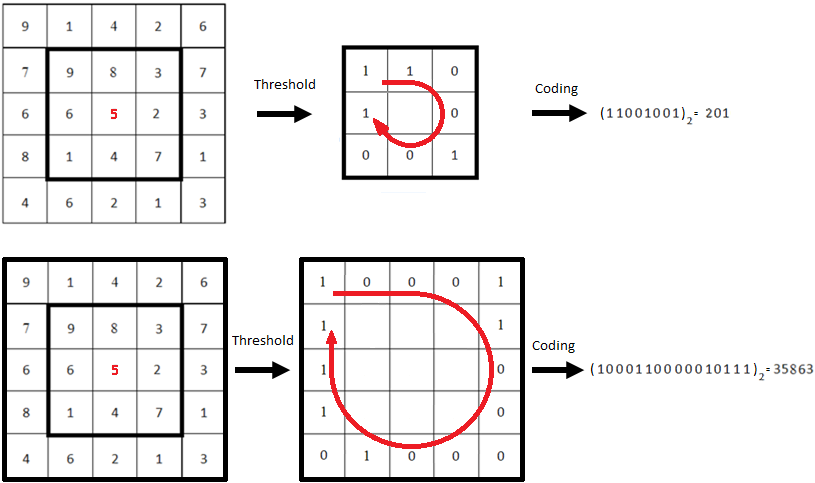
\includegraphics[width=0.90\textwidth]{images/LBP}
	\caption[LBP operators.]{\label{fig:LBP}The LBP operators $LBP_{8,1}$  and $LBP_{16,2}$, respectively  }
\end{figure}

\section{Feature Selection} \label{FS}
A further step, not always present on a CAD system, is the feature selection, a process commonly used in pattern recognition that allows determining the most relevant features reducing the size of the vectors associated with the objects. The feature selection aims to reduce the dimensionality eliminating both the redundant features, that represent information derived from other, both the features that are irrelevant for
the analysis. The "ideal" approach would be to test all the possible subsets of features, using them as input to the classification algorithm of interest and select the subset that allows obtaining the best results. This approach in most cases is not applicable. There are several techniques for the selection of characteristics, that can be grouped into three categories:
\begin{itemize}
	\item embedded methods: the selection is internal to the classification algorithm that takes advantage of internal knowledge of the classifier, such as the weight used to induce the model \cite{Duda}
	\item filter methods: also known as scheme-independent selection, because the selection is made in advance, with a method independent from the classification algorithm that will be applied subsequently using some measure of distance or correlation \cite{Yu}
	\item wrapper methods: also known as scheme-specific selection, because the selection is performed making a comparison between different subsets of features, investigated with approaches of sequential forward or backward selection \cite{Kittler}, according to the classification algorithm that will be applied later.
\end{itemize}
Generally, the wrapper methods perform better than the other methods, as they are optimized for a specific classifier, but they are computationally eligible only for small feature vectors.
On the other hand, there are different approaches called, by many authors, "feature selection" that do not perform a proper features selection, but rather a dimensionality reduction through projection or combination. The Principal Component Analysis (\acs{PCA}) \cite{Wold} is the most popular technique for the reduction of dimensionality. Its purpose is to find a set of orthogonal vectors in the feature space corresponding to the directions along which the data have the highest variance. Projecting the data from their original space to the orthogonal complement permits the dimensionality reduction of the features. 
The advantages of the PCA is that it can deal with large datasets both in objects and variables reducing the redundancy. Moreover, it does not make particular assumptions on the data, and so it can be applied to all datasets. The most significant disadvantage arises from the fact that PCA does not select the features, but it creates new ones combining the original. This procedure dramatically affects the control over the single feature, that is particularly important in image processing where features are extracted directly from the image and thus it is essential to establish which are determinant for the task of classification, in order to avoid the extraction of insignificant features.  

\chapter{Classification}
Once the features have been extracted from cells, they must be inserted in a process that classifies cells based on medical concepts. Given a collection of records, each one composed by a set of features $x$ and by a label of class $y$, the goal is to define a function or classification model, that associates a class label $y$ to each set of attributes $x$. A classification model is a tool to describe and classify the data of a specific domain. It is possible thanks to a training set, namely a set of training samples in which the values of the class labels are well known. So, the relations between attributes and class labels can be identified and encoded in a model, through a learning algorithm. This model must be able not only to describe the training set but also to predict the class of new records not yet labeled correctly. Literature comprises several classification algorithms, but the most used on medical images are following listed:
\begin{itemize}
	\item Nearest Neighbour
	\item Decision Trees
	\item Bayesian Classifier    
	\item Neural Network
	\item Support Vector Machine
\end{itemize}
Moreover, machine learning methods are generally divided into {\it supervised} and {\it unsupervised learning} algorithms, although there are many nuances. In supervised learning, a model is presented with a dataset $\mathcal{D} = \{{\bf x}, y\}^{N}_{n = 1}$ of input features ${\bf x}$ and label $y$ pairs, where $y$ typically represents an instance of a fixed set of classes. In the case of regression tasks $y$ can also be a vector with continuous values. Supervised training typically amounts to finding model parameters $\Theta$ that best predict the data based on a loss function $L(y, \hat{y})$. Here $\hat{y}$ denotes the output of the model obtained by feeding a data point ${\bf x}$ to the function $f({\bf x}; \Theta)$ that represents the model.
Unsupervised learning algorithms process data without labels and are trained to find patterns, such as latent subspaces. Examples of traditional unsupervised learning algorithms are principal component analysis and clustering methods. Unsupervised training can be performed under many different loss functions. One example is reconstruction loss $L({\bf x}, \hat{{\bf x}})$ where the model has to learn to reconstruct its input, often through a lower-dimensional or noisy representation.

\section{Nearest Neighbor} \label{kNN}
The Nearest Neighbour classifier uses the concept of proximity to classify a new record, based on the samples provided by the training set that are similar to it. Each instance of the training set is a point in an n-dimensional space, where $n$ is the number of features. When NN has to classify a new record, it calculates its distance from each training set sample. Then, the $k$ examples of the training set closer to the new record, called k-Nearest Neighbors (k\acs{NN})  \cite{Cover}, are identified and used to assign the class label prevailing among kNN to the new record. However, there may be problems in the choice of $k$, in fact, if this value is too small, there is a high sensitivity to noise, but if it is too large, there may be examples not similar enough to the record to be classified, among the kNN. One way to reduce the influence of the parameter $k$ is to calculate the prevailing class by assigning a different weight to each of the first neighbors according to its distance from the record to be classified. This type of classifier is the simplest among those listed, as it does not require the induction of a model from the training set, which is used in the classification step to compare the new records with the known ones. In contrast to the saved resources for the construction of the model, the classification of a new record, however, is rather expensive. Indeed, the proximity between the new record and the known examples of the training set must be calculated every time.

\section{Decision Trees} \label{DT}
Decision Trees \cite{Quinlan} are decision support tools that use a tree-like graph or decision model for classification. The goal is to create a model that predicts the value of a target variable by learning simple decision rules inferred from the data features. Thus, during the classification of a new record, the decision tree represents a flowchart-like structure in which each internal node represents a test on an attribute, and each branch represents the outcome of the test. Obviously, each leaf node represents a class label, and the decision is taken after computing all attributes. The paths from the root to the leaf nodes represent the classification rules. The greatest advantage of decision trees is that they are simple to understand and interpret, but they can be complex with a high number of attributes. In particular, having more attributes conducts to a deeper tree and, therefore, the decision rules become more complex and the model fitter.
Among disadvantages, there is that decision tree can create too complex trees that do not produce a suitable generalization of the data, generating overfitting, even though the greatest one is that the same classification rules can be expressed with different decision trees. Thus finding the optimal decision tree is known to be an NP-complete problem under several aspects of optimality and even for simple concepts. This problem is generally mitigated by training multiple trees in an ensemble learner, where the features and samples are randomly sampled with a replacement strategy.

\section{Bayesian Classifier} \label{NB}
The Bayesian classifiers are based on probabilistic relations between the class labels and feature values of the record. Considering the features of a record as random variables a Bayesian network can be used to plot the conditional dependencies among a set of random variables. It is an acyclic and directed graph in which the nodes represent random variables, and the arcs represent dependency relationships between the variables. Each node of the network is associated with a probability table containing the a priori probability if that node does not depend on any other node, or the conditional probability if the node depends on a set of other nodes. Thus, given a training sample, it must be found the Bayesian network that best describes the conditional dependencies between variables. Once defined the network, the process of classification of a new record entails the calculation of the posterior probability for each class and the selection of the class for which the probability is the highest. The induction of the network that best describes a given training set involves the definition of network structure and the estimation of probabilities values table associated with each node of the network. In a general case, this is an intractable problem, but some algorithms induce Bayesian classification models introducing appropriate simplifying assumptions on the network topology. The simplest among the Bayesian classifiers is the so-called Naive Bayes  \cite{Duda}, \cite{Langley} and is based on the assumption that the features are conditionally independent, given the value of the class. In this way the a priori probability of the class and the conditional probabilities of the class features can be easily estimated from the training sample. With the Naive Bayes method, the model is not significantly influenced by either the noise, which is mediated through the calculation of probabilities or by any unnecessary features, for which the probabilities are distributed in an almost uniform way. Despite its simplicity, the Bayesian classifier can perform accurate classifications but only if the features are discriminatory.

\section{Artificial Neural Network} \label{ANN}
Artificial Neural Networks (\acs{ANN}) classifiers are the most used in medical applications. They are networks that emulate the behavior of the human brain, composed of a set of nodes that are interconnected by links to which a weight is associated. In ANNs, as in biological systems, learning corresponds to change the weight values of the connections between nodes. Given a training sample, the weights of the model are first initialized randomly and then iteratively adjusted, so that the output of the model appears consistent with the values of the label class. The simplest ANNs are composed of two levels, the input level, and the output level. The input layer contains a node for each numerical features, while the categorical features require more nodes, for example, a feature with $n$ possible values can be transformed into $n$ binary variables. The output layer, on the other hand, can contain only one node, if the problem of classification is binary and $k$ nodes if the class label can assume $k$ values. There are also multilevel ANNs whose structures present additional hidden layers between the input layer and the output layer. The number of hidden layers is often determined by trial and error, in fact, typically the correct number of hidden layers is found starting from a network with a high number of layers and nodes, and it progressively decreases the model complexity. Network training involves the adjustment of the weights with the aim to minimize the internal error. This process is costly, especially if the network topology is complex, even if the classification process is rapid. The model is susceptible to noise because the weights are adjusted for each instance of the training sample. On the contrary, the irrelevant or redundant features do not significantly affect the model, since the corresponding weights are typically tiny.

\section{Support Vector Machine} \label{SVM}
Support Vector Machines (\acs{SVM}) are supervised learning models with associated learning algorithms that analyze data used for classification and regression analysis. They have been designed for binary classification problems, so with only two classes, but it can also be extended to multi-class problems. The SVM binary classification is based on the mapping of input vectors in a high dimensionality features space, induced by a kernel function. The learning algorithm produces an optimal hyperplane of separation between the two classes. The SVM can perform linear and nonlinear discrimination, according to the kernel function. It is possible to find a kernel function for which the parameters of the model can be induced without an explicit mapping data. The induction of the model in this way is formulated as an optimization problem, in which it is possible to find quite efficiently a global minimum for the objective function. The SVM provides extreme flexibility both because it is possible to make use of different types of kernels and because it is possible to define a hyperplane for separating classes which guarantees a certain tolerance with respect to noise, using a soft margin instead of a hard margin. For an optimization problem, it becomes changing the constraint value with the $c$ value, that can be increased to obtain less training error. Kernel methods use other parameters for the creation of the separating hyperplane. The Gaussian Radial Basis Function (\acs{RBF}) is one of the most used kernels performing a non-linear separation defined by the radius  $\gamma$ of the RBF. Other kernels are the quadratic kernel, the polynomial kernel that can be defined with different order $p$ and the Multilayer Perceptron kernel (MLP) that instead can be defined for different slope $\alpha$ and the intercept constant $\beta$. The multi-class problem is solved by building many different binary classifiers and then combine them. The most used strategies are the combinations one-vs-one and one-vs-all. 

\subsection{One-vs-all SVM} 
The one-vs-all approach, also known as one-vs-rest, is the first and the most intuitive approach to extend the SVM to multi-class problems. The basic idea of the one-vs-all approach is straightforward. In fact, for a multi-class problem having $m$ classes, it consists on training $m$ different binary SVM classifiers where each one of them separates one class from all the other $m-1$ classes. Then, in the testing phase the class label is assigned taking into account the decision of every $m$ classifiers. The most common practice is to assign the class label $i$, where $i$ is the classifier that maximizes the separation between the class $i$ from the rest. Another common practice is to use binary trees to arrange the $m-1$ binary SVM; the path from the root node to a leaf determines the class label. In the best scenario, only one comparison is needed, while in the worst case  $m-1$ comparisons are needed. The problem encountered with binary tree SVM is that there are $\prod_{i=3}^{m}2i-3$ possible ways to construct a tree for a multi-class problem. Thus, for a multi-class problem with a huge value of $m$, analyzing all the possible solutions is impossible.

\subsection{One-vs-one SVM}
The one-vs-one approach is another commonly used SVM strategy but, differently from the one-vs-all approach, for a multi-class problem having $m$ classes, it consists on training $\frac{m(m-1)}{2}$ different binary SVM classifiers, where each one of them separates a class from another one. In this case, combining the results from individual binary SVM classifiers becomes more complex. The simplest way to obtain the predicted class label is to use the majority voting, counting the votes given by each binary classifier and assigning the class label that has the highest number of votes. However, the voting process could produce ambiguous results (e.g., tie cases).
For this reason, a common practice is to use the majority voting strategy combined with the maximum separation strategy, assigning the class label $i$, if the result of the binary classifier produces the highest number of $i$ votes with the maximum separation between $i$ class and each of the other classes. Another common practice consists in arranging all the $\frac{m(m-1)}{2}$ binary SVM classifiers in a Directed Acyclic Graph (\acs{DAG}) structure with the same number of nodes. The test phase starts at the root node and continues until a leaf node, representing the predicted class label, is reached. Thus, only $m-1$ comparisons are needed, completely avoiding tie cases, but the problem is encountered just during the construction of the DAG. , in this case, there are several ways to construct the DAG structure, and each one of them may produce different classification results and when the number of classes is high, testing all possible orders is impossible.

\section{Deep learning methods}
\label{sec:neuralnets}

\subsection{Neural Networks}
Neural networks are a type of learning algorithm which forms the basis of most deep learning methods. A neural network comprises of neurons or units with some activation $a$ and parameters $\Theta = \{\mathcal{W}, \mathcal{B}\}$, where $\mathcal{W}$ is a set of weights and $\mathcal{B}$ a set of biases. The activation represents a linear combination of the input ${\bf x}$ to the neuron and the parameters, followed by an element-wise non-linearity $\sigma(\cdot)$, referred to as a transfer function: 
\begin{equation}
a = \sigma({\bf w}^{T}{\bf x} + b).
\end{equation}
Typical transfer functions for traditional neural networks are the sigmoid and hyperbolic tangent function.  The multi-layered perceptrons (MLP), the most well-known of the traditional neural networks, have several layers of these transformations:
\begin{equation}
f({\bf x}; \Theta) = \sigma( {\bf W}^{T}\sigma({\bf W}^{T} \ldots \sigma({\bf W}^{T} {\bf x} + b)  ) + b).
\end{equation}
Here, ${\bf W}$ is a matrix comprising of columns ${\bf w}_{k}$, associated with activation $k$ in the output. Layers in between the input and output are often referred to as 'hidden' layers. When a neural network contains multiple hidden layers it is typically considered a 'deep' neural network, hence the term 'deep learning'.

At the final layer of the network the activations are mapped to a distribution over classes $P(y | {\bf x}; \Theta)$ through a {\it softmax} function:
\begin{equation}
P(y | {\bf x}; \Theta) = \text{softmax}({\bf x}; \Theta) = \frac{e^{{\bf w}_{i}^{T}{\bf x} + b_{i}}}{\sum^{K}_{k = 1} e^{{\bf w}_{k}^{T}{\bf x} + b_{k}}},
\end{equation}
where ${\bf w}_{i}$ indicates the weight vector leading to the output node associated with class $i$. 

Maximum likelihood with stochastic gradient descent is currently the most popular method to fit parameters $\Theta$ to a dataset $\mathcal{D}$. In stochastic gradient descent a small subset of the data, a mini-batch, is used for each gradient update instead of the full data set. Optimizing maximum likelihood in practice amounts to minimizing the negative log-likelihood:
\begin{equation}
\arg \min_{\Theta} - \sum^{N}_{n = 1} \log\big[ P(y_{n}| {\bf x}_{n}; \Theta) \big].
\end{equation}
This results in the binary cross-entropy loss for two-class problems and the categorical cross-entropy for multi-class tasks. A downside of this approach is that it typically does not optimize the quantity we are interested in directly, such as area under the receiver-operating characteristic (ROC) curve or common evaluation measures for segmentation, such as the Dice coefficient. 

Currently, the most popular models are trained end-to-end in a supervised fashion, greatly simplifying the training process. The most popular architectures are convolutional neural networks (CNNs) and recurrent neural networks (RNNs). CNNs are currently most widely used in (medical) image analysis, although RNNs are gaining popularity. 

\subsection{Convolutional Neural Networks (CNNs)}
There are two key differences between MLPs and CNNs. First, in CNNs weights in the network are shared in such a way that it the network performs convolution operations on images. This way, the model does not need to learn separate detectors for the same object occurring at different positions in an image, making the network equivariant with respect to translations of the input. It also drastically reduces the amount of parameters (i.e.\ the number of weights no longer depends on the size of the input image) that need to be learned. 

At each layer, the input image is convolved with a set of $K$ kernels  $\mathcal{W} = \{ {\bf W}_{1}, {\bf W}_{2}, \ldots, {\bf W}_{K} \} $ and added biases $\mathcal{B} = \{b_{1}, \ldots, b_{K}\}$, each generating a new feature map ${\bf X}_{k}$. These features are subjected to an element-wise non-linear transform $\sigma(\cdot)$ and the same process is repeated for every convolutional layer $l$:
\begin{equation}
\label{eq::mapping_cnn}
{\bf X}_{k}^{l} = \sigma\big( {\bf W}_{k}^{l -1} \ast {\bf X}^{l -1} + b_{k}^{l-1} \big).
\end{equation}

The second key difference between CNNs and MLPs, is the typical incorporation of pooling layers in CNNs, where pixel values of neighborhoods are aggregated using a permutation invariant function, typically the max or mean operation. This induces a certain amount of translation invariance and again reduces the amount of parameters in the network. At the end of the convolutional stream of the network, fully-connected layers (i.e.\ regular neural network layers) are usually added, where weights are no longer shared. Similar to MLPs, a distribution over classes is generated by feeding the activations in the final layer through a softmax function and the network is trained using maximum likelihood. 

\subsection{Deep CNN Architectures}
Given the prevalence of CNNs in medical image analysis, we elaborate on the most common architectures and architectural differences among the widely used models. 

\subsubsection{General classification architectures}
LeNet \cite{Lecu98} and AlexNet \cite{Kriz12}, introduced over a decade later, were in essence very similar models. Both networks were relatively shallow, consisting of two and five convolutional layers, respectively, and employed kernels with large receptive fields in layers close to the input and smaller kernels closer to the output. AlexNet did incorporate rectified linear units instead of the hyperbolic tangent as activation function.

After 2012 the exploration of novel architectures took off, and in the last three years there is a preference for far deeper models. By stacking smaller kernels, instead of using a single layer of kernels with a large receptive field, a similar function can be represented with less parameters. These deeper architectures generally have a lower memory footprint during inference, which enable their deployment on mobile computing devices such as smartphones. \cite{Simo14} were the first to explore much deeper networks, and employed small, fixed size kernels in each layer. A 19-layer model often referred to as VGG19 or OxfordNet won the ImageNet challenge of 2014. 

Since 2014, the performance on the ImageNet benchmark has saturated and it is difficult to assess whether the small increases in performance can really be attributed to 'better' and more sophisticated architectures. The advantage of the lower memory footprint these models provide is typically not as important for medical applications. Consequently, AlexNet or other simple models such as VGG are still popular for medical data, though recent landmark studies all use a version of GoogleNet called Inception v3 \cite{Guls16}. Whether this is due to a superior architecture or simply because the model is a default choice in popular software packages is again difficult to assess. 

\subsection{Recurrent Neural Networks (RNNs)}
\label{sec:rnns}
Traditionally, RNNs were developed for discrete sequence analysis. They can be seen as a generalization of MLPs because both the input and output can be of varying length, making them suitable for tasks such as machine translation where a sentence of the source and target language are the input and output. In a classification setting, the model learns a distribution over classes $P(y | {\bf x}_{1}, {\bf x}_{2}, \ldots, {\bf x}_{T}; \Theta)$ given a sequence ${\bf x}_{1}, {\bf x}_{2}, \ldots, {\bf x}_{T}$, rather than a single input vector ${\bf x}$.

The plain RNN maintains a latent or hidden state ${\bf h}$ at time $t$ that is the output of a non-linear mapping from its input ${\bf x}_{t}$ and the previous state ${\bf h}_{t-1}$:
\begin{equation}
{\bf h}_{t} = \sigma({\bf W}{\bf x}_{t} + {\bf R}{\bf h}_{t - 1} + {\bf b}),
\end{equation}
where weight matrices ${\bf W}$ and ${\bf R}$ are shared over time. For classification, one or more fully connected layers are typically added followed by a softmax to map the sequence to a posterior over the classes. 
\begin{equation}
P(y | {\bf x}_{1}, {\bf x}_{2}, \ldots, {\bf x}_{T}; \Theta) = \text{softmax}( {\bf h}_{T}; {\bf W}_{out}, {\bf b}_{out}).
\end{equation}

Although initially proposed for one-dimensional input, RNNs are increasingly applied to images. In natural images 'pixelRNNs' are used as autoregressive models, generative models that can eventually produce new images similar to samples in the training set. 

\section{Model Evaluation} \label{ME} % DONE
The performance of the classification models is then evaluated on the basis of percentage of records correctly classified on a test set with a known class label. Therefore, \textit{accuracy} and the \textit{error rate} of the model can be calculated by comparing the known class labels, and the classifiers predicted labels. A binary problem is composed of positive and negative classes and it can be evaluated with the following measures: True Positive (\acs{TP}) indicates the number of positives records correctly classified as positives, True Negative (\acs{TN}) measure indicates the number of negatives records correctly classified as negative, False Positive (\acs{FP}) measure is the number of negative records misclassified as positive and, finally, False Negative (\acs{FN}) measure is the number of positive records misclassified as negative. In this way, the accuracy of the error rate can be written as in (\ref{accuracy}) and (\ref{error}):

\begin{equation}\label{accuracy}
accuracy= \frac{TP + TN}{TP + TN + FP + FN}    
\end{equation}

\begin{equation}\label{error}
error rate= \frac{FP + FN}{TP + TN + FP + FN}    
\end{equation}

Differently from binary classification ones, if the problem presents an uncommon number of classes the accuracy and the error rate typically are not good measures of model performance. In this case, the most used measures are the \textit{True Positive Rate} (\acs{TPR}) also called \textit{sensitivity} or \textit{recall} (r) (\ref{TPR}), the \textit{True Negative Rate} (\acs{TNR}) also called \textit{specificity} (\ref{TNR}), the \textit{False Positive Rate} (\acs{FPR}) (\ref{FPR}), the \textit{False Negative Rate} (\acs{FNR}) (\ref{FNR}) and the \textit{precision} (p) (\ref{precision}). Precision and recall are used if the correct classification of positive instances is considered more important or interesting, according to the faced problem. Indeed, a good model should be able to maximise both measures. For this reason, another important metric is frequently used: the \textit{F-measure} or \textit{F-score} (\ref{Fmeasure}).

\begin{equation}\label{TPR}
TPR = r = \frac{TP}{TP + FN}    
\end{equation}

\begin{equation}\label{TNR}
TNR = \frac{TN}{TN + FP}    
\end{equation}

\begin{equation}\label{FPR}
FPR= \frac{FP}{TN + FP}    
\end{equation}

\begin{equation}\label{FNR}
FNR= \frac{FN}{TP + FN}    
\end{equation}

\begin{equation}\label{precision}
p = \frac{TP}{TP + FP}    
\end{equation}

\begin{equation}\label{Fmeasure}
F\mbox{-}score = \frac{2rp}{r + p}    
\end{equation}

It is worth noting that the same measures are also used for segmentation evaluation. Actually, if any manually segmented images or ground-truth are available, a pixel-wise evaluation can be made in order to assess if a pixel has been correctly included in the region which it belongs (TP), it has been correctly excluded from the region (TN), it has been erroneously included in the region (FP) or it has been wrongly excluded from the region (FN).

The performance of a model may not depend only on the type of classification algorithm but also by other factors such as the size or distribution of the classes in the training and test set. In particular, if the dataset has reduced size, the performances are more related to the specific composition of the samples, and a higher variance characterizes them. Some methods are quite useful to extract a representative test set, from the original dataset, able to assess the performance of the model. They are:
\begin{itemize}
	\item Holdout: a part of the available samples, the training set, is used to train the model while another part, the test set, is used for its evaluation. Holdout involves a reduction of examples available for training and addiction due from specific partition created. To ensure that the training set and the test set are uniformly representative, the partition can be made by using a stratified sampling process.
	\item Repeated Holdout: the holdout method is iterated $k$ times, in order to avoid control over the number of times that each record is used for training and testing. The accuracy and error rate are calculated averaging the $k$ iteration results.
	\item Cross-Validation: the examples available are divided into $k$ sub-sets of equal dimension. The process of training and evaluation of the model is repeated $k$ times, each time using $k-1$ different sub-sets for training and one sub-set for the test. As for Repeated Holdout, the accuracy and error rate are calculated averaging the $k$ iteration results, but in this case, the final results are more stable since the test sets are mutually exclusive and cover the entire initial sample.
	\item Leave-one-out: a special case of cross-validation in which $k$ is equal to the number of records. Thus during the training phase, the largest possible number of examples is used, and each test set contains only one record. This approach provides exhaustive results, but it is computationally costly.
\end{itemize}